\documentclass[11pt]{scrartcl}

%---------------------------------
% Sprache, Schriften, Zeichensatz
%---------------------------------
\usepackage[ngerman]{babel}

\usepackage[T1]{fontenc}
\usepackage[utf8]{inputenc}

\usepackage{csquotes}	% für babel

%---------------------------------
% Datum/Zeit
%---------------------------------
\usepackage[ngerman]{datetime}

\newdateformat{germandate}{\THEDAY. \monthname[\THEMONTH] \THEYEAR}

%---------------------------------
% BibLaTeX: Online-Quellen
%---------------------------------
\usepackage[backend=biber, style=numeric, sorting=none]{biblatex}
% sorting=none -> keine Sortierung, Standard ist alphabetisch

% TexMaker-Kommando für bib(la)tex: "biber" %
% (Original-Einstellung für bibtex: "bibtex" %.aux

\addbibresource{BachelorthesisQuellen.bib}

%---------------------------------
% Meta Variables
%---------------------------------
\newcommand{\MetaInstitute}{Hochschule Bremen}
\newcommand{\MetaUnit}{Fakultät 4 -- Elektrotechnik und Informatik}
\newcommand{\MetaTitle}{Anwendung von Hardware-Raytracing zur Optimierung der Treffererkennung}
\newcommand{\MetaSubtitle}{Eine Untersuchung zur Leistungssteigerung und Präzisionsverbesserung in Echtzeit-Anwendungen}
\newcommand{\MetaTask}{Bachelorthesis}
\newcommand{\MetaAuthorName}{Kevin Niclas}
\newcommand{\MetaAuthorSurname}{Kügler}
\newcommand{\MetaAuthor}{\MetaAuthorName~\MetaAuthorSurname}
\newcommand{\MetaStudentNumber}{\textit{399027}}
\newcommand{\MetaExaminer}{Prof. Dr. Martin Hering-Bertram}
\newcommand{\MetaCoExaminer}{Prof. Dr. Volker Paelke}
\newcommand{\MetaStudyProgram}{Internationaler Studiengang Medieninformatik (B.Sc.)}
\newcommand{\MetaDate}{\germandate\today}
\newcommand{\MetaVersion}{1.00}

%---------------------------------
% Content Variables
%---------------------------------

%---------------------------------
% Glossar & Abkürzungen
%---------------------------------
\usepackage[acronym, nonumberlist]{glossaries}
\makeglossaries

\newglossaryentry{raytracing}{
	name={Raytracing},
	description={Eine Technik zur Bildsynthese, bei der Lichtstrahlen in einer 3D-Szene simuliert werden}
}

\newglossaryentry{physik-engine}{
	name={Physik-Engine},
	description={Software zur Simulation physikalischer Effekte in Echtzeit-Anwendungen}
}

\newglossaryentry{vulkan}{
	name={Vulkan},
	description={Eine hardwarenahe Programmierschnittstelle für Grafikkarten, die Entwicklern präzise Kontrolle über die Hardware ermöglicht}
}

\newglossaryentry{acceleration-structures}{
	name={Acceleration Structures},
	description={Spezielle Datenstrukturen, die zur Optimierung des Raytracings verwendet werden}
}

\newglossaryentry{bvh}{
	name={Bounding Volume Hierarchy (BVH)},
	description={Eine Baumstruktur von Bounding Volumes zur schnellen Kollisionserkennung}
}

\newglossaryentry{dlss}{
	name={Deep Learning Super Sampling (DLSS)},
	description={Ein Machine-Learning-Algorithmus von NVIDIA zur Bildskalierung und -verbesserung}
}

\newglossaryentry{hitboxen}{
	name={Hitboxen},
	description={Vereinfachte geometrische Formen zur Kollisionserkennung in Videospielen}
}

\newglossaryentry{ray-queries}{
	name={Ray Queries},
	description={Eine vereinfachte Form von Raytracing-Pipelines, die innerhalb von Shadern ausgeführt werden}
}

\newglossaryentry{command-buffer}{
	name={Command Buffer},
	description={Speicher für eine Abfolge von Befehlen, die an die GPU gesendet werden}
}

\newglossaryentry{descriptor-sets}{
	name={Descriptor Sets},
	description={Eine Sammlung von Ressourcenbindepunkten in Vulkan, die in Shadern verwendet werden}
}

\newglossaryentry{pipelines}{
	name={Pipelines},
	description={Grafische oder Berechnungspipelines, die in Vulkan verwendet werden, um Shader und andere Grafikanweisungen zu verwalten}
}

\newglossaryentry{shader}{
	name={Shader},
	description={Programme, die auf Grafikhardware ausgeführt werden, um verschiedene Berechnungen durchzuführen}
}

\newglossaryentry{descriptor-pools}{
	name={Descriptor Pools},
	description={Speicherpools zur Optimierung der Erstellung von Descriptor Sets in Vulkan}
}

\newglossaryentry{memory-barriers}{
	name={Memory Barriers},
	description={Synchronisationsmechanismen in Vulkan, die sicherstellen, dass Speicheroperationen abgeschlossen sind}
}

\newglossaryentry{physical-device}{
	name={Physical Device},
	description={Repräsentiert eine oder mehrere Hardware-Komponenten in Vulkan}
}

\newglossaryentry{logical-device}{
	name={Logical Device},
	description={Eine Abstraktion in Vulkan, die Ressourcen allokiert und einen Zustand besitzt}
}

\newglossaryentry{queue}{
	name={Queue},
	description={Eine Warteschlange in Vulkan, die zur Verwaltung von Befehlen dient}
}

\newglossaryentry{pipeline}{
	name={Pipeline},
	description={Eine Kombination aus Shadern in Vulkan, die vorab kompiliert wird, um die Performance zu erhöhen}
}

\newglossaryentry{shader-storage-buffer-object}{
	name={Shader Storage Buffer Object (SSBO)},
	description={Ein Speicherobjekt, das zum Datentransfer zwischen CPU und Shader verwendet wird}
}

\newacronym{api}{API}{Application Programmable Interface}
\newacronym{aabb}{AABB}{Axis-aligned Bounding Box}
\newacronym{bv}{BV}{Bounding Volume}
\newacronym{boundingvh}{BVH}{Bounding Volume Hierarchy}
\newacronym{cpu}{CPU}{Central Processing Unit}
\newacronym{deeplss}{DLSS}{Deep Learning Super Sampling}
\newacronym{fps}{FPS}{Frames per Second}
\newacronym{gpu}{GPU}{Graphics Processing Unit}
\newacronym{ml}{ML}{Machine Learning}
\newacronym{rt-kerne}{RT-Kerne}{Raytracing-Kerne}
\newacronym{spir-v}{SPIR-V}{Standard Portable Intermediate Representation-V}
\newacronym{ue5}{UE5}{Unreal Engine 5}
\newacronym{vram}{VRAM}{Video Random Access Memory}
\newacronym{blas}{BLAS}{Bottom-Level Acceleration Structure}
\newacronym{tlas}{TLAS}{Top-Level Acceleration Structure}
\newacronym{ssbo}{SSBO}{Shader Storage Buffer Object}
\newacronym{pci-e}{PCI-E}{Peripheral Component Interconnect Express}
\newacronym{glsl}{GLSL}{OpenGL Shading Language}
\newacronym{cpu-l2-cache}{L2 Cache}{Second-Level Cache der CPU}
\newacronym{queue-family}{Queue Family}{Gruppe von Queues in Vulkan, die ähnliche Aufgaben ausführen}
\newacronym{compute-shader}{Compute Shader}{Shader für allgemeine Berechnungen auf der GPU}


\glsaddall

%---------------------------------
% Anhänge
%---------------------------------
\usepackage[titles]{tocloft}

% Definiere das Anhangsverzeichnis
\newlistof{appendices}{app}{}
\newcommand{\appendixitem}[1]{%
	\refstepcounter{appendices}
	\addcontentsline{app}{appendices}{\protect\numberline{\theappendices} #1}%
	\section*{#1}
}
\renewcommand{\cftsecfont}{\normalfont\sffamily\bfseries} % Setzt die Schriftart für \section auf normal
\renewcommand{\cftsubsecfont}{\normalfont} % Setzt die Schriftart für \subsection auf normal
\renewcommand{\cftsubsubsecfont}{\normalfont} % Setzt die Schriftart für \subsubsection auf normal
\renewcommand{\cftsecpagefont}{\normalfont\sffamily\bfseries} % Setzt die Seitenzahl für \section auf normal
\renewcommand{\cftsubsecpagefont}{\normalfont} % Setzt die Seitenzahl für \subsection auf normal
\renewcommand{\cftsubsubsecpagefont}{\normalfont} % Setzt die Seitenzahl für \subsubsection auf normal


%---------------------------------
% Querverweise
%---------------------------------
% Hyperref (sollte unbedingt vor geometry-Paket geladen werden)
% für Anzeige in Acrobat (pdfstartview)
\usepackage[bookmarks=false,
pdfstartview=FitV,
pdfhighlight={/I},
colorlinks = false,
linkcolor = blue,
urlcolor  = blue,
citecolor = blue,
pdfborder={0 0 0},
german]{hyperref}

\hypersetup{
	pdfauthor   = {\MetaAuthor},
	pdftitle    = {\MetaTitle},
	% pdfsubject  = {\MetaUnit, \MetaTask},
	pdfsubject  = {\MetaTask},
	pdfkeywords = {\MetaTitle, \MetaUnit, \MetaInstitute},
	% pdfkeywords = {\MetaTitle, \MetaUnit, \MetaTask, \MetaInstitute},
}

% Für bessere Fußnoten
\usepackage{fnpct}

% Für Verweise mit Angabe des Typs des referenzierten Objekts (z.B. "Kapitel")
\usepackage[ngerman]{cleveref}

\crefname{section}{Kapitel}{Kapitel}	% Anpassung der Typbezeichnungen
\crefname{subsection}{Abschnitt}{Abschnitte}
\crefname{lstlisting}{Listing}{Listing} % neue Typbezeichnung


%---------------------------------
% Grafiken, Farben
%---------------------------------
\usepackage{graphicx}
\graphicspath{ {./Figures/} }

\usepackage{xcolor}

\definecolor{keyword}{HTML}{0000FF}	% Farben für Listings
\definecolor{string}{HTML}{D12F1B}
\definecolor{comment}{HTML}{008400}
\definecolor{lightgrey}{rgb}{0.99,0.99,0.99}

\definecolor{note}{rgb}{1,1,0.8}		% Farbe für Notizen


%---------------------------------
% Seitenlayout: Abmessungen
%---------------------------------
% Option für zusätzlichen Rand zum Binden: bindingoffset
% Default-Verhältnis von oberem (innerem) zu unterem (äußerem) Rand: 2:3
%\usepackage[top=3.6cm,bottom=4.50cm,left=2.3cm,bindingoffset=0.5cm, pdftex,twoside,a4paper]{geometry}
\usepackage[top=3.6cm,bottom=4.50cm,left=2.3cm,bindingoffset=0.5cm, pdftex,a4paper]{geometry}

\setlength{\parindent}{6mm} 
\setlength{\parskip}{0.2cm} 


% Raum für Notizen mit note-Paket
%\usepackage[top=3.6cm,bottom=4.5cm,right=4cm,bindingoffset=0.5cm,twoside]{geometry}

% "includemp" zieht Notizbereich (marginpar) von Druckbereich ab:
%\usepackage[top=3.6cm,bottom=4.50cm,left=2.3cm,bindingoffset=0.5cm,marginparwidth=3cm, includemp, pdftex,twoside,a4paper]{geometry}

%---------------------------------
% Seitenlayout: Kopf- und Fußzeilen
%---------------------------------
\usepackage[headsepline]{scrlayer-scrpage}

\clearpairofpagestyles
\automark[section]{section}	% Anzeige der "section" in der Kopfzeile
\lohead{\headmark}
\cofoot[\pagemark]{\pagemark} % Anzeige der Seitenzahl in der Fußzeile
\pagestyle{scrheadings}

%\pagestyle{empty}


%---------------------------------
% Seitenlayout: Überschriften
%---------------------------------
\addtokomafont{subsubsection}{\normalfont\sffamily}	% subsubsection nicht bold
\addtokomafont{paragraph}{\normalfont\sffamily}	% paragraph nicht bold


%---------------------------------
% Enumeration mit Zahlen auf allen Ebenen (für Gliederung)
%---------------------------------
\usepackage{enumitem}

\newlist{gliederung}{enumerate}{4}
\setlist[gliederung]{label*=\arabic*.}


%---------------------------------
% Listings
%---------------------------------
\usepackage{listings}

\lstset{
	language=C++,
	basicstyle=\ttfamily,
	showstringspaces=false, % lets spaces in strings appear as real spaces
	breaklines=true,
	breakatwhitespace=false,
	columns=fixed,
	keepspaces=true,
	keywordstyle=\color{keyword},
	stringstyle=\color{string},
	commentstyle=\color{comment},
	frame=tb,	% Rahmen = single
	%  framerule=1pt,
	showstringspaces=false,
	basicstyle=\footnotesize\ttfamily,
	backgroundcolor=\color{lightgrey},
	numbers=left,
	tabsize=4
}



%---------------------------------
% To Do Notes
%---------------------------------
\usepackage[textwidth=3.5cm, backgroundcolor=note]{todonotes}


%---------------------------------
% Tabellen
%---------------------------------
\usepackage{multirow}
%usepackage{array}
\usepackage{makecell}
\usepackage{booktabs}	% http://ctan.org/pkg/booktabs

\newcommand{\tabitem}{~~\llap{\textbullet}~~}


%---------------------------------
% Floating environments genauer positionieren
%---------------------------------
\usepackage{float}

%---------------------------------
% Wasserzeichen
%---------------------------------
%\usepackage{draftwatermark}
%
%\SetWatermarkText{DRAFT}
%\SetWatermarkScale{6}

%---------------------------------
% Commands
%---------------------------------
\newcommand{\HRule}{\rule{\linewidth}{0.2mm}}	% Horizontal line for title page
\newcommand{\qto}[1]{\glqq #1\grqq}				% Anführungszeichen

\newcommand{\urlMitUmlauten}[2]{\texttt{\href{#1}{#2}}}				% URL mit Umlauten

% Abkürzungen (mit korrekten Abständen)
\usepackage{xspace}
\newcommand{\zB}{\mbox{z.\,B.}\xspace}
\newcommand{\dH}{\mbox{d.\,h.}\xspace} % Kommando \dh ist schon definiert
\newcommand{\ggf}{ggf.\xspace}
\newcommand{\evtl}{evtl.\xspace}
\newcommand{\bzw}{bzw.\xspace}


%---------------------------------
% Document start
%---------------------------------
\begin{document}
	
	%---------------------------------
	% Titlepage
	%---------------------------------
	\begin{titlepage}
		\shortdate % Use Short Date
		\center % Center everything on the page
		
		%~\\[1cm]
		
		%---------------------------------
		% HEADER SECTIONS
		%---------------------------------
		
		\begin{figure}[h!]
			\centering
			\resizebox{12cm}{!}{
				
\includegraphics[width=90mm,keepaspectratio]{./Images/HSBLogo.png}
			}
		\end{figure}
		
		\vspace{-0.5cm}
		\textsc{\Large \MetaInstitute}\\[0.2cm] % Major heading such as course name
		\textsc{\Large \MetaUnit}%[2.5cm] % Major heading such as course name
		
		\textsc{\large \MetaStudyProgram}\\[1.5cm]
		
		%---------------------------------
		% DOCUMENT TYPE SECTION
		%---------------------------------
		\textsc{\LARGE \MetaTask}\\[1.5cm] % Minor heading such as course title
		
		%---------------------------------
		% TITLE SECTION
		%---------------------------------
		%	\HRule \\[0.5cm]
		%	{
		%		\LARGE \bfseries \MetaTitle \\[0.50cm] % Title of your document
		%		\par
		%	}
		%	\HRule \\[1.5cm]
		\HRule \\[0.5cm]
		{
			\LARGE \bfseries \MetaTitle \\[0.50cm] % Title of your document
			\LARGE \bfseries -- \MetaSubtitle\ -- \\[0.50cm] % Title of your document
			\par
		}
		\HRule \\[1.5cm]
		
		%---------------------------------
		% AUTHOR SECTION
		%---------------------------------
		\large 
		\MetaAuthor\ (\MetaStudentNumber)

		~\\

		Prüfer: \MetaExaminer
		
		Zweitprüfer: \MetaCoExaminer
		
		%---------------------------------
		% DATE SECTION
		%---------------------------------
		\vspace*{\fill}
		{
			\large \MetaDate\ (Version \MetaVersion)
		}
	\end{titlepage}
	
	\pagebreak
	\tableofcontents
	\pagebreak
	
	% Neue Seite beginnen und Text vertikal und horizontal zentrieren
	\newpage
	\thispagestyle{empty} % Optional: keine Seitenzahl anzeigen
	
	\vspace*{\fill}
	\begin{center}
		Folgenden Personen gebührt mein besonderer Dank
		
		\vspace{0.5cm}
		Alexander Stöwing, für seine unermüdliche Hilfe bei Fragen jeglicher Art
		
		 und
		
		meiner wunderbaren Frau, Natalie, für ihre mentale Unterstützung, auch wenn es zwischendurch sehr schwer wurde
		
		und
		
		meiner wundervollen Tochter, Lucy
	\end{center}
	\vspace*{\fill}


	\pagebreak
	%---------------------------------
	% EINLEITUNG
	%---------------------------------
	\section{Einleitung}
	
	In der Welt der Videospiele und erweiterten Realitätsanwendungen (XR) stellen die steigende Komplexität und die Anforderungen an die Treffererkennung eine Herausforderung dar. Traditionelle CPU-basierte Methoden stoßen zunehmend an ihre Grenzen, was die Systemperformance und die Spielerfahrung beeinträchtigt. Diese Arbeit erforscht die Möglichkeit, die Treffererkennung durch den Einsatz von Raytracing-Kernen (RT-Kerne) auf GPUs zu realisieren, um die Präzision zu steigern und die CPU-Last zu verringern.

	\subsection{Problemstellung}
	
	Die Problematik der Treffererkennung in interaktiven Echtzeit-Umgebungen verschärft sich mit der zunehmenden Komplexität von Spielwelten und der fortlaufenden Entwicklung realistischerer 3D-Modelle. Die CPU ist in einer modernen Game-Engine oft mit mehreren Aufgaben belastet, einschließlich KI-Steuerung, Spiellogik und der Verwaltung von Benutzerinputs, wodurch die Ressourcen für die Treffererkennung limitiert sind. 
	
	Die traditionelle Hit-Scan-Methode, die auf der CPU ausgeführt wird, stößt bei der Skalierung auf Grenzen. Typischerweise werden Hitboxen in Form von Quadern, Sphären und Kapseln zur Vereinfachung des 3D-Modells verwendet. Der Strahl von seinem Startpunkt in die gegebene Richtung projiziert. Trifft der Strahl auf eine Hitbox, wird die Berechnung beendet und Trefferinformationen zurückgegeben. Alternativ kann das 3D-Modell selber als Hitbox fungieren, allerdings mit deutlich erhöhtem Rechenaufwand. 
	
	Dies führt zu einem Dilemma: Die Erhöhung der Präzision der Treffererkennung verlangt mehr Rechenzeit, was wiederum die Bildwiederholrate und damit die Immersion und Interaktion beeinträchtigen kann.
	
	\subsection{Lösungsansatz}
	
	Im Rahmen der Arbeit wird das Hit-Scan-Verfahren auf die GPU verlagert, um die Rechenleistung der spezialisierten RT-Kerne moderner Grafikkarten zu nutzen. Diese Anpassung zielt darauf ab, die Geschwindigkeit und Präzision der Treffererkennung zu steigern, während gleichzeitig die Belastung der CPU reduziert wird.
	
	Die Verlagerung des GPU-basierten Hit-Scan-Verfahrens soll mit der Programmierschnittstelle (API) Vulkan\footnote{\url{https://www.vulkan.org/}}, speziell Vulkan Ray Queries, realisiert werden. Ray Queries ermöglichen den Einsatz der RT-Kerne außerhalb von Rendering-Shadern. Sie können für beliebige Zwecke benutzt werden. So auch für Treffererkennung.\cite{Koch2020}
	
	Mehrere Testszenen mit variierender Anzahl von statischen 3D-Modellen sollen der Evaluierung dienen: Durch Vergleichen der Performance des Verfahrens auf der GPU mit dem bestehenden CPU-basierten Ansatz in Unreal Engine 5 (UE5)\footnote{\url{https://.unrealengine.com/en-US/unreal-engine-5}}, einer 2022 veröffentlichten Game-Engine die von Epic Games entwickelt wurde, wird überprüft ob die GPU-Implementierung eine schnellere Verarbeitung ermöglicht. Dieser Vergleich soll die Vorteile der GPU-Nutzung für Echtzeit-Treffererkennung in interaktiven Anwendungen verdeutlichen. Der GPU-basierte Ansatz wird in einer zuvor eigens entwickelten Rendering-Engine, genannt Prism, verwirklicht.

	\pagebreak
	\section{Grundlagen}
	
	Dieses Kapitel widmet sich den für diese Arbeit relevanten Themen und beschreibt Grundlagen dieser. Dazu gehört das Raytracing, eine Methode zur realistischen Bildsynthese, die Lichtstrahlen in einer 3D-Szene simuliert. Weiterhin wird die Anwendung von Raytracing in Physik-Engines zur Kollisionserkennung in Videospielen beschrieben. Zudem wird Vulkan, eine leistungsfähige und hardwarenahe Programmierschnittstelle für Grafikkarten, behandelt, die Entwicklern präzise Kontrolle über die Hardware ermöglicht.
	
	\subsection{Raytracing}
	
	Andrew Glassner beschreibt Raytracing als Technik zur Bildsynthese, das Erstellen eines 2D Bildes aus einer 3D Welt\cite{Glassner2019}. Ein Monitor besteht aus unzähligen Pixeln mit jeweils einem Farbwert und Glassner erklärt, dass jedes Pixel eine Lochkamera repräsentiert aus der die 3D Welt betrachtet wird. Raytracing ahmt Photonen aus der realen Welt nach und gibt so dem Pixel seinen Farbwert basierend auf den Farbwerten der Objekte auf die das digitale Photon, auch Strahl genannt trifft, abprallt und irgendwann zurück Richtung Lochkamera fliegt.
	
	Seit Immel et al. und James Kajiya zur gleichen Zeit auf der SIGGRAPH\footnote{\url{https://www.siggraph.org/}} 1986 verschiedene Rendertechniken mit ihrer Rendering-Gleichung vereinheitlicht haben\cite{ImmelEtAl1986, Kajiya1986}, hat sich Raytracing stetig weiterentwickelt und gilt in der Videospielbranche als heiliger Gral des Renderings\cite{Corporation2018}. Nichts in Spielen ist realistischer als eine virtuelle Welt die von unserer nicht mehr zu unterscheiden ist. Trotz unzähliger Optimierungstechniken sowie Durchbrüche bei der Hardwareentwicklung waren Grafikkarten nicht stark genug Raytracing in 30 oder mehr Frames per Second (FPS)\footnote{dt. Bilder pro Sekunde} in gängigen Bildschirmauflösungen darzustellen. Erst die Erfindung von Raytracing-Kernen in Kombination mit Machine Learning (ML) Algorithmen zum hochskalieren von Bildern, genannt Deep Learning Super Sampling (DLSS)\cite{NvidiaDlss2024} auf den Turing-Grafikkarten der Firma NVIDIA\footnote{\url{https://www.nvidia.com}} löste das Problem der niedrigen FPS\cite{Corporation2018}. Seitdem haben sich beide Technologien weiterentwickelt. DLSS Frame Generation\cite{NvidiaDlss2024} erlaubt die Generierung von Bildern anstatt diese nur hoch zu skalieren. Weiterhin ist mit DLSS Ray Reconstruction\cite{NvidiaDlss2024} eine ML-basierte Möglichkeit geschaffen um die Anzahl an Strahlen welche in die 3D Szene geschossen werden verringert, aber dennoch das finale Bild annähernd korrekt darstellt.
	
	\subsection{Physik-Engine}
	
	Doch Raytracing ist nicht nur relevant für die Bildsynthese. Physik-Engines nutzen die Technik in abgewandelter Form ebenfalls zum projizieren von Strahlen zur Treffererkennung. In Videospielen verwendete Waffen wie Gewehre oder Bögen sind oft nicht vollständig über Zeit hinweg simuliert, sondern werden innerhalb eines Berechnungszyklus, genannt Tick, durch die 3D-Szene projiziert. Trifft die Kugel dabei ein Objekt kann sie absorbiert werden, es durchstoßen oder abprallen. Ersterer Fall ist der relevanteste. Die Physik-Engine berechnet beim Aufprall zudem die Kräfte welche auf das Objekt einwirken und wendet sie auf selbiges an, je nach Konfiguration. Um den Berechnungsaufwand gering zu halten werden bei der Überprüfung ob die Kugel ein Objekt trifft nicht alle Polygone zur Strahl-Polygon-Verschneidung, wie beispielsweise durch den Möller–Trumbore-Schnittalgorithmus\cite{MoellerTrumbore1997}, herangezogen sondern lediglich vereinfachte geometrische Formen, genannt Hitboxen, wie Quader, Sphären oder Kapseln. Diese lassen sich mathematisch darstellen ohne dass Polygone benötigt werden\cite{Ericson2004}. Dieses Verfahren der Treffererkennung ist seit Jahrzehnten Standard in der Videospielbranche. 
	
	Eine weitere Optimierung sind Bounding Volumes (BV). Anstatt den Strahl mit jedem einzigen 3D-Modell und dessen Polygonen, die in fotorealistischen Spielen in die Zehn- bis Hunderttausende gehen können, innerhalb der 3D-Szene auf einen Treffer zu prüfen, werden die 3D-Modelle mit Bounding Volumes umgeben. Die bekannteste Form sind Axis-aligned Bounding Boxes (AABB). Das 3D-Modell wird hierbei von einem an den Achsen des Koordinatensystems ausgerichteten Quaders vollständig umschlossen. Im ersten Schritt wird der Strahl nun auf Kollision mit allen AABBs geprüft. Gibt es einen Treffer werden die einzelnen Polygone mit dem Strahl auf einen Schnittpunkt überprüft. Dies verringert den Berechnungsaufwand signifikant. Dennoch ist der Aufwand bei sehr detaillierten 3D-Modellen weiterhin hoch, besonders in Anbetracht der immer steigenden Polygon-Anzahl. Als Lösung dafür gibt es ein Subset der BVs: Bounding Volume Hierarchies (BVH). Die 3D-Modelle werden in mehrere in einer Baumstruktur angeordneten Bounding Volumes unterteilt. Wenngleich es üblich ist, dass einzelne BVs sich nicht überlappen und die 3D-Modellgeometrie so in mehreren BVs enthalten ist, kann dies je nach Anwendungs- oder Optimierungsfall durchaus vorkommen. Anders als in beispielsweise Octrees, erfunden von Donald Meagher\cite{Meagher1980}, sind BVHs weder an eine Unterteilungstiefe gebunden noch müssen die Kind-Knoten innerhalb des Vater-Knotens positioniert sein.\cite{Ericson2004}
	
	Bounding Volume Hierarchies sind Gegenstand vieler Forschungen. Aktuelle Veröffentlichungen umfassen die Nutzung von Machine Learning zur Erstellung von BVHs, wie Philippe Weier et al. zeigen\cite{Weier2024} sowie Mochi, eine Collision Detection-Engine von Mandarapu et al. welche die RT-Kerne der Grafikkarte nutzt\cite{Mandarapu2024}.
	
	Die zuvor angesprochenen RT-Kerne bilden das Prinzip der Bounding Volume Hierarchies und der Strahl-Polygon-Verschneidung in Hardware ab. John Burgress beschreibt in seinem Artikel \textit{RTX on - The NVIDIA Turing GPU} das Funktionsprinzip der RT-Kerne: Ein Shader mit Strahl-Informationen übergibt diese an die RT-Kerne, welche den generierten BVH solange durchlaufen bis entweder eine Verschneidung mit einem Polygon festgestellt wurde oder der Strahl ins Nichts ging. Anschließend wird das Ergebnis an weitere Shader zurückgegeben. Abbildung \ref{fig:rtcoresexplained} beschreibt diesen Prozess im unteren Teil. Die obere Hälfte zeigt den Prozess auf Grafikhardware ohne RT-Kerne. Laut Burgress ist der Performance-Gewinn gegenüber dem Raytracing ohne RT-Kerne Sieben Mal höher.\cite{Burgess2020} Auf Abbildung \ref{fig:rtcoresbvhexplained} im Anhang ist eine Visualisierung des BVH-Algorithmus zu finden.
	
	\begin{figure}[h]
		\centering
		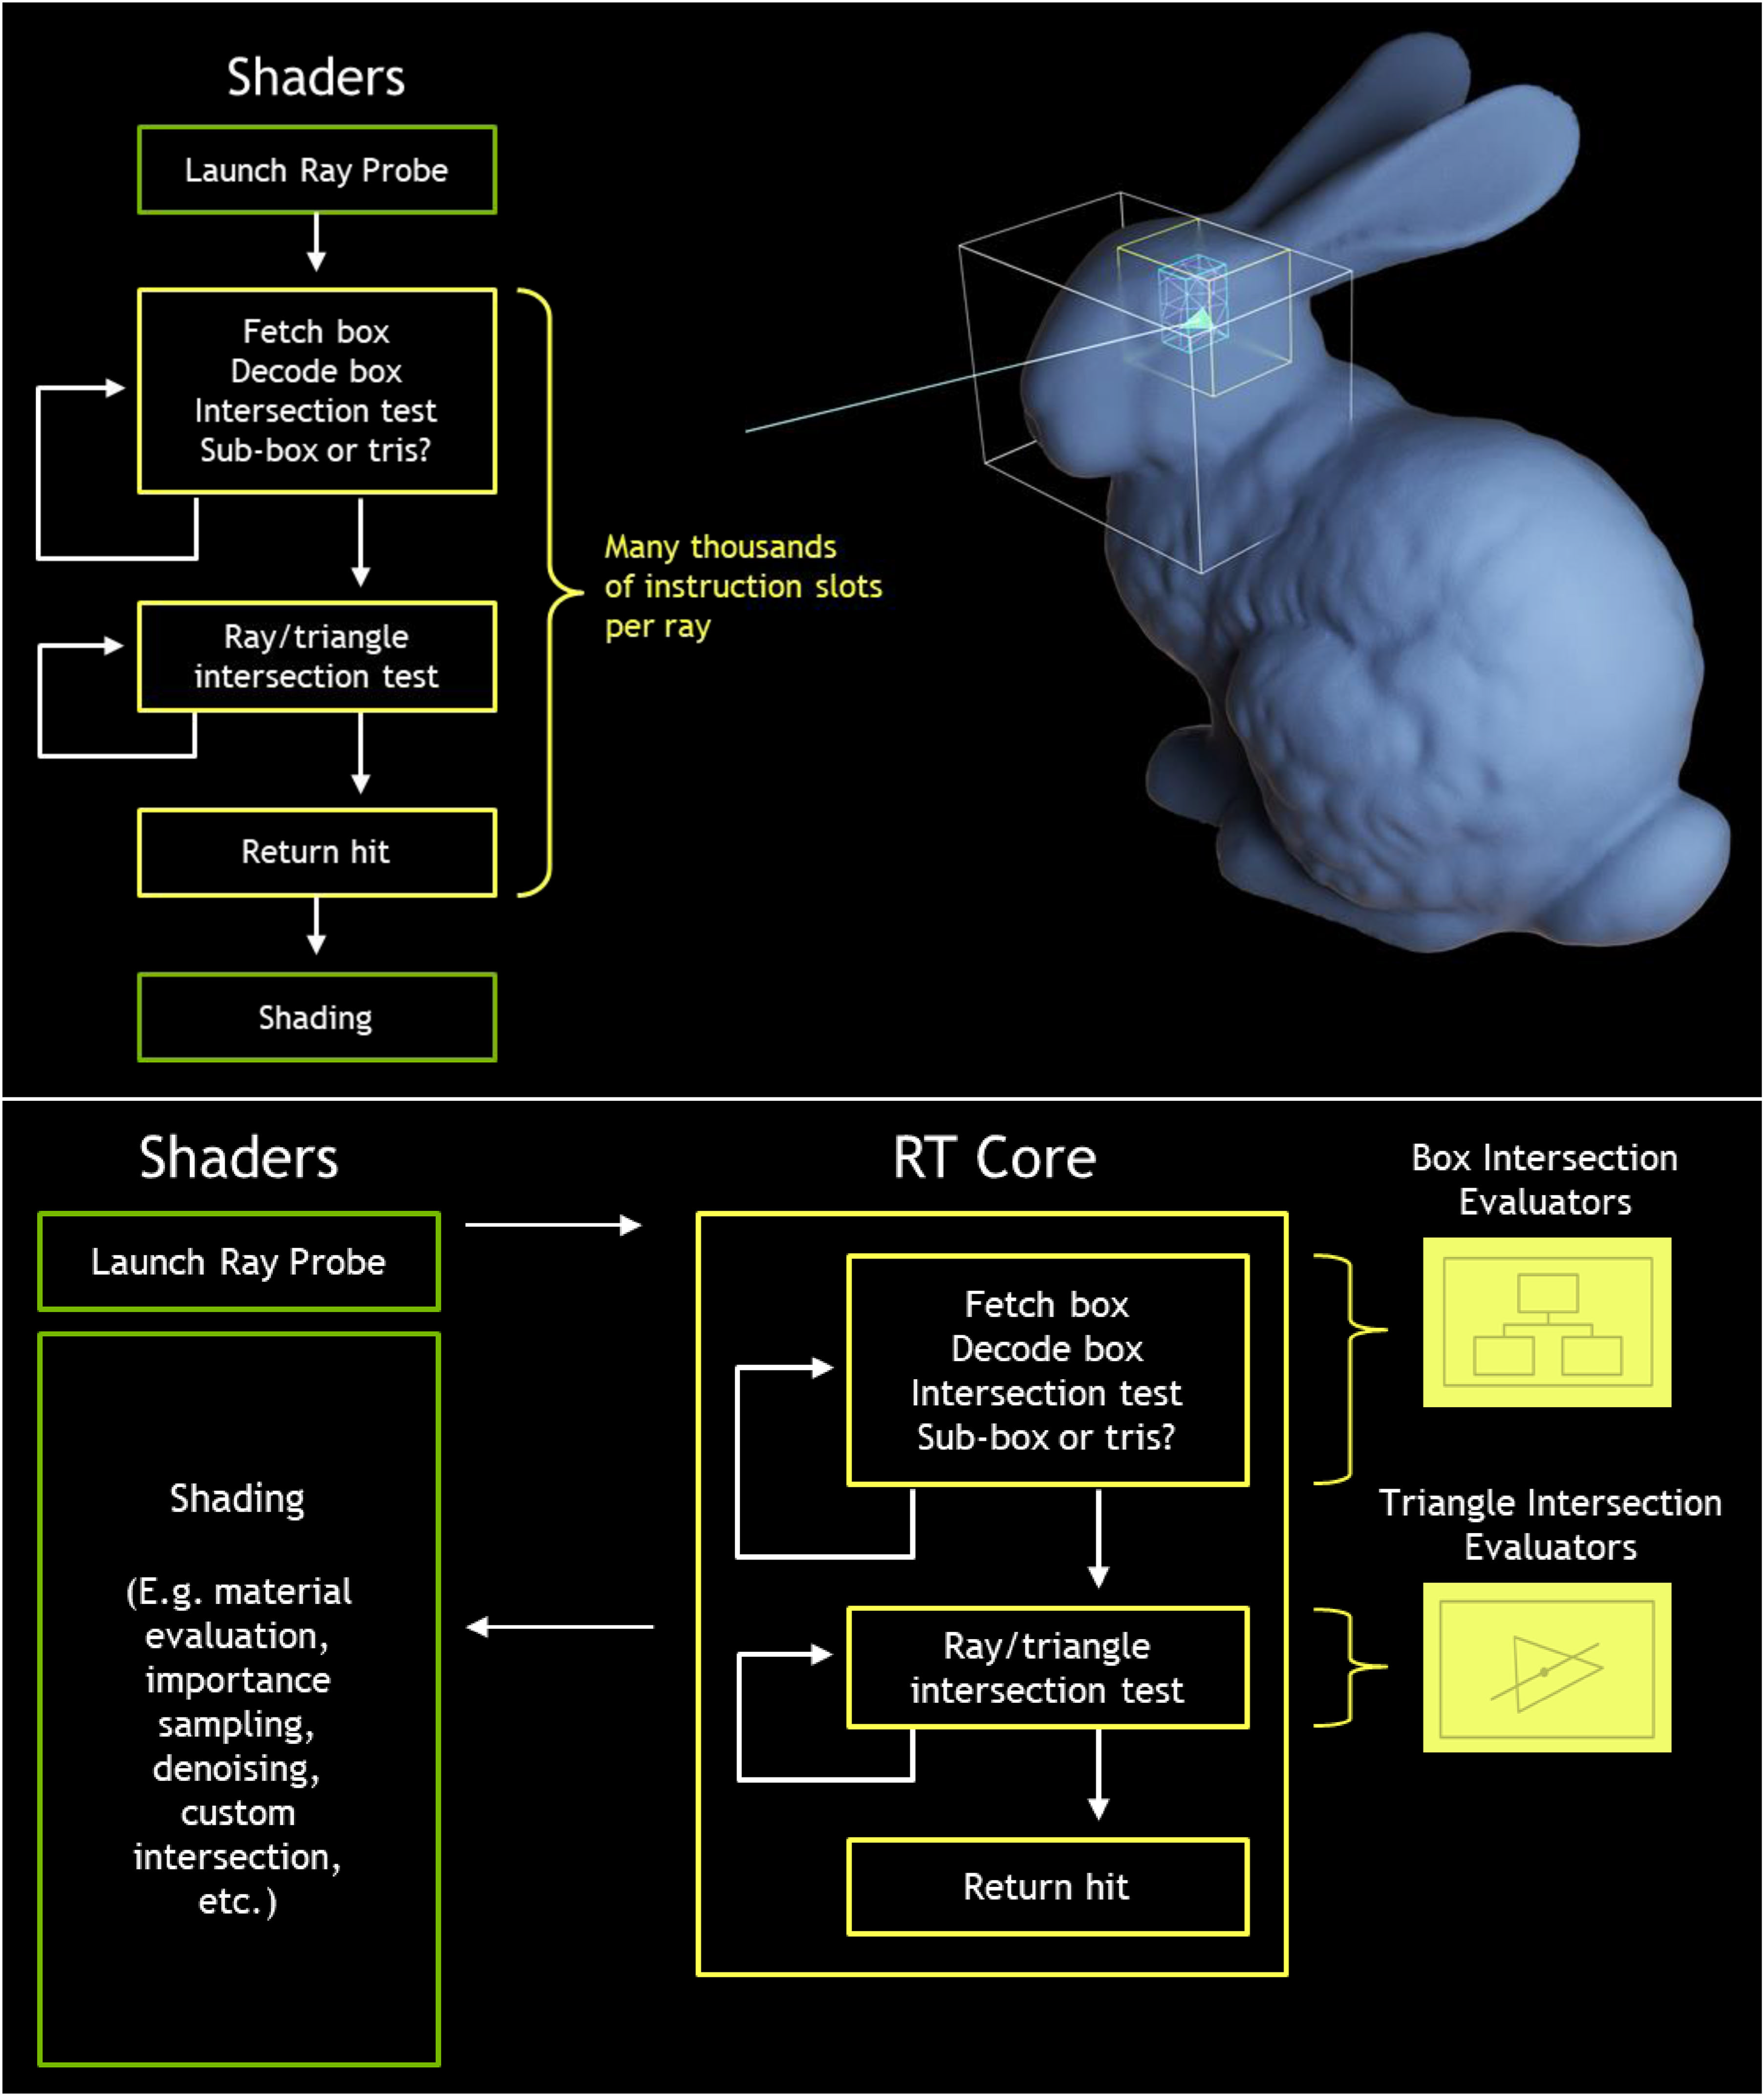
\includegraphics[width=0.7\linewidth]{Figures/rt_cores_explained}
		\caption[Funktionsweise der RT-Kerne]{Funktionsweise der RT-Kerne; oberer Teil zeigt Raytracing ohne RT-Kerne, unterer zeigt diesen mit RT-Kernen\cite{Burgess2020}}
		\label{fig:rtcoresexplained}
	\end{figure}
	
	Die Nutzung der RT-Kerne außerhalb des 3D-Renderings ist ebenfalls Gegenstand mehrerer Arbeiten. So haben Steinberger et al. 2019 die Verwendung von RT-Kernen zur Punktlokalisierung innerhalb von unstrukturierten Tetraeder-Meshes erforscht und festgestellt, dass die Implementation mit RT-Kernen schneller war\cite{Steinberger2019}. Yuhao Zhu hingegen hat 2022 eine Methode zur Leistungssteigerung der Nachbarn-Klassifikation unter Verwendung von RT-Kernen vorgeschlagen\cite{zhu2022rtnn}. Experimentelle Ergebnisse zeigten eine 2,2-65-fache Steigerung der Performance gegenüber bestehenden Programmbibliotheken.
	
	\subsection{Vulkan}
	
	Vulkan ist eine 2016 veröffentlichte, quelloffene in C geschriebene Programmierschnittstelle (API\footnote{Application Programmable Interface}) zur Grafikkarte und wird von der Khronos Group\footnote{\url{https://www.khronos.org/}} entwickelt. Anders als OpenGL\footnote{\url{https://www.opengl.org/}} ist Vulkan hardwarenäher und erlaubt dem Programmierer genauere Kontrolle über die Grafikkarte. Ältere APIs wie OpenGL übernehmen viele Funktionen wie Fehlerbehandlung, Synchronisation und Speichermanagement die in Vulkan vom Programmierer explizit gesteuert werden müssen und verringert so den Programmieraufwand. Dies hat jedoch zur Folge, dass Detailoptimierungen schwieriger sind. Der Programmierer ist daher auf die Qualität der API angewiesen.\cite{Sellers2017} Die Hardwarenähe und Ausführlichkeit von Vulkan haben jedoch den Nachteil, dass, wenn bestimmte Funktions-Parameter oder -Aufrufe falsch gesetzt sind oder fehlen, dies zu Programmabstürzen oder fehlerhaften Bildausgaben führen kann. Weiterhin erzeugt die Ausführlichkeit bereits bei kleinen Programmen wie dem \textit{Hello World Polygon} für über 1000 Zeilen Quellcode. Andererseits wird Vulkan wegen diesen Eigenschaften von professionellen 3D-Programmierern geschätzt und gilt mittlerweile als Standard in der Spieleindustrie und ist auf fast jeder Betriebssystem-Plattform. Eine ähnliche API stellt Microsoft bereit: DirectX 12\footnote{\url{https://gpuopen.com/directx12/}}.
	
	Vulkan kann mehrere Grafikkarten unabhängig voneinander ansprechen, ein zentraler Unterschied zu OpenGL. Allerdings ist es nicht nur auf Grafikkarten beschränkt. Ähnliche Verarbeitungs-Hardware wie Digitale Signalprozessoren und reine Compute-Shader-Karten die universelle mathematische Berechnungen durchführen kann ebenfalls angesprochen werden\cite{Sellers2017}. Um mit Hardware zu kommunizieren bedarf es zweier Vulkan-Konstrukte. Das Physical Device repräsentiert eine oder mehrere Hardware-Komponenten und stellt lediglich einen Ansteuerpunkt im Code dar. Erst Mithilfe des Logical Device, welches tatsächliche Ressourcen allokiert und einen Zustand besitzt, kann das Physical Device gezielt abgefragt sowie gesteuert werden. Dies ist ein grundlegender Unterschied zu OpenGL bei dem die Ressourcen und der Zustand global sind. Ein Physical Device kann zu mehr als einem Logical Device gehören.\cite{Sellers2017, VulkanPhysicalDevice, VulkanLogicalDevice}
	
	Einer der Grundeigenschaften von Vulkan ist die Erweiterbarkeit. Die API ist in zwei Bereiche unterteilt: \textit{Core} und \textit{Extensions}. Jede Hardware die mit Vulkan interagieren kann, muss alle Inhalte des \textit{Core} in ihrem Treiber implementiert haben. Dagegen sind \textit{Extensions} optional. Hardware-Treiber können eine beliebige Anzahl an \textit{Extensions} bereitstellen. Auch muss der Vulkan-Treiber selbst diese \textit{Extension} anbieten.\cite{Sellers2017, VulkanExtensions}
	
	Anders als OpenGL setzt Vulkan auf ein rechtshändiges kartesisches 3D-Koordinatensystem und besitzt weitere feine Unterschiede bei Koordinatensystem-Berechnungen.\cite{Harmer2023}
	
	Um Arbeit auf der Hardware verrichten zu lassen, stellt Vulkan Queues bereit. Eine Queue ist einer Queue Family zugehörig welche mithilfe des Physical Device abgefragt und anschließend bei der Erstellung des Logical Device angefragt werden können. Da Vulkan Primär für das Rendering und Compute-Operationen entwurfen wurde, sind die beiden bekanntesten Queue Families die Graphics Queue Family und Compute Queue Family\cite{VulkanQueues}. Anders als viele andere Operationen erzeugt der Programmierer Queues nicht selbst. Der Treiber übernimmt dies beim Erstellen des Logical Device\cite{Sellers2017}.
	
	Konkrete Arbeitsbefehle werden durch Command Buffer aufgezeichnet und gespeichert. Diese Command Buffer können je nach gesetztem Flag bei Erstellung mehrmals abgespielt werden, was wertvolle Zeit spart. Die Command Buffer werden in die zuvor erklärten Queues eingereiht. Die Queues arbeiten die Command Buffer meist nach \textit{First In - First Out} Prinzip ab, die Grafikkarte kann allerdings diese Reihenfolge brechen wenn sich Optimierungsmöglichkeiten offenbaren\cite{VulkanQueues}.\cite{Sellers2017}
	
	Die Verwaltung von RAM\footnote{dt. Arbeitsspeicher} und Video-RAM (VRAM)\footnote{dt. Grafikspeicher} in Vulkan ist in zwei Arten unterteilt: Host Memory und Device Memory\cite{Sellers2017}. Beide Arten müssen durch den Programmierer verwaltet werden, ähnlich dem Speichermodell in C++. Ein Garbage-Collector existiert nicht, kann jedoch manuell implementiert werden. Dieses explizite Speichermodell erlaubt gezielte und performante Verwaltung des Grafikspeichers. Zuvor in OpenGL wurde der Speicher durch den Grafiktreiber allokiert und musste von diesem abgeschätzt werden. Um Speicherblöcke zwischen CPU und GPU zu transferieren wird Memory Mapping verwendet. Speicherzugriff innerhalb derselben Hardwarekomponente, beispielsweise des CPU L2 Cache, ist sehr schnell. Kommunikation zu einer anderen Hardwarekomponente ist bedeutend langsamer da hierbei anstatt auf internen Speicher innerhalb derselben Komponente auf den Peripheral Component Interconnect Express (PCI-E)-Bus als Trägermedium zurückgegriffen werden muss. Der PCI-E-Bus kann unter umständen von weiterer anderer Hardware benutzt werden welche ggf. viel Bandbreite des Bus in Besitz nehmen.\cite{VulkanMemory}
	
	Multithreading spielt in Vulkan eine wichtige Rolle. Viele Performance-kritische Operationen sind in Vulkan nicht synchron, d.h. dass mehrere Threads gleichzeitig auf dieselbe Ressource schreiben und lesen können\cite{Sellers2017}. Dies kann zu inkonsistenten Zuständen der Daten führen und so für Fehler und Abstürze sorgen. Um dies zu vermeiden gibt es mehrere Arten von Synchronisationsmechanismen in Vulkan\cite{VulkanSync}.
	Die einfachste Art ist auf das gesamte Logical Device zu warten. Eine solche Warteoperation ist teuer, denn die CPU muss in diesem Fall darauf warten dass das Logical Device komplett im Leerlauf ist. Eine zweite Möglichkeit stellt das Warten auf eine Queue dar. Hier muss lediglich darauf gewartet werden, dass alle Command Buffer innerhalb der Queue abgearbeitet wurden.
	
	Für gezieltes Warten stellt Vulkan Barriers zur Verfügung. Es gibt mehrere Arten von Barriers, eine davon sind sogenannte Memory Barriers. Mithilfe dieser kann sichergestellt werden, dass Speicheroperationen wie der Transfer zwischen zwei Speicherpuffern abgeschlossen sind, ein Command Buffer beispielsweise darauf zugreifen darf.\cite{VulkanMemorySyncBlog}
	
	Shader stellen eine essentielle Komponente zum Verrichten von Arbeit auf Grafik- und Compute-Hardware dar. Sie bestehen aus Code einer C-ähnlichen Sprache, der OpenGL Shading Language (GLSL)\cite{Rost2004}. Es gibt mehrere Shader-Arten. Darunter Vertex-Shader zum verarbeiten der 3D-Modelldaten, Fragment-Shader die einzelne Pixel berechnen und Compute-Shader mit denen beliebige mathematische Berechnungen und andere nicht Rendering-relevante Funktionen ausgeführt werden können.\cite{Sellers2017} Im Gegensatz zu OpenGL verlangt Vulkan Shader in einem Bytecode-Format, {Standard Portable Intermediate Representation-V (SPIR-V). Dieses Zwischenformat ermöglicht es Vulkan komplexe High-Level Compiler aus den Hardware-Treibern auf externe Compiler-Programme auszulagern. Dadurch muss lediglich der standardisierte Bytecode auf der Hardware ausgeführt werden was so die Laufzeit-Performance steigert.\cite{VulkanSpirv}

	Buffer sind eine fundamentale Ressource in Vulkan und bilden mit dem Buffer Memory die primäre Möglichkeit Daten zu verwalten. Buffer sind ein linearer Speicherblock und können vielseitig eingesetzt werden. Beispiele umfassen Vertex Buffer für 3D-Modelldaten sowie Index Buffer die Vertices in Vertex Buffer referenzieren. Auch gibt es Shader Storage Buffer Objects (SSBO) die zum Datentransfer zwischen CPU und Shader benutzt werden.\cite{Sellers2017}
	Um diese Memory Handles innerhalb von Vulkan und der Hardware zu nutzen sind Descriptors nötig. Sie dienen als Bindeglied zwischen Shader und Vulkan-API sowie VRAM. Descriptors sind in Descriptor Sets gebündelt welche wiederrum an einzelne Shader gebunden sind. In Shadern lassen sich die gebundenen Descriptor Sets ansteuern und Lese- sowie Schreiboperationen auf ihnen ausführen. Die ist ein Vorteil, da diese bis zum Binden an einen anderen Shader verfügbar bleiben und dadurch aktiv im Speicher verbleiben. Descriptor Sets werden auf Grundlage einer Art Blaupause, den Descriptor Set Layouts generiert. Durch die Vorgabe eines nicht veränderbaren Layouts kann der Hardware-Treiber die Ressourcennutzung optimieren. Zur weiteren Leistungssteigerung werden Descriptor Sets aus Descriptor Pools angefragt. Pooling ist in der Programmierung ein verbreitetes Mittel um die Erzeugung von Objekten zu optiminieren. Jede Speicherallokierung ist verhältnismäßig teuer. Um dies zu umgehen kann eine feste Menge an Objekten vorallokiert werden. Wird eines dieser Objekte, beispielsweise ein Descriptor Set benötigt, gibt der Descriptor Pool eines zur Verwendung frei. Wird es nicht mehr benötigt, nimmt der Pool das Set wieder an sich. Bei der Freigabe werden jegliche eventuell vorhandenen Zustände des Descriptor Sets zurückgesetzt um einen konsistenten Datenzustand zu gewährleisten.\cite{Sellers2017, VulkanDescriptorPools}
	
	Shader und Descriptor Sets sind aus Gründen der Performance an Pipelines gebunden. Jede Kombination aus Shadern wird einer Pipeline zugeordnet. Es gibt mehrere Arten von Pipelines, die wichtigsten sind Graphics Pipelines für das Rendering und Compute Pipelines für allgemeine mathematische Berechnungen. Soll beispielsweise ein 3D-Modell mit Texturen und prozedural generierten Polygonen gerendert werden, wird eine Graphics Pipeline mit einem Vertex-, Fragment- und Mesh-Shader benötigt. letzterer erzeugt Geometrie prozedural ohne vorige Erzeugung eines Vertex-Buffers. Der Vorteil an Pipelines besteht darin, dass sie bei Initialisierung von Vulkan vorab kompiliert werden. Dies erhöht die Performance zur Laufzeit und verhindert stottern durch Shader- und Pipeline-Kompilierung.\cite{Sellers2017, VulkanPipelines}

	\pagebreak
	\section{Konzeption}
	
	In modernen Game-Engines wird die Treffererkennung typischerweise durch die folgende Funktion realisiert:
	\begin{lstlisting}[caption={\textit{traceRay} Funktion in Pseudocode},label={lst:listing-traceraypseudo}]
	void traceRay(Origin, Direction, minDistance, maxDistance)	\end{lstlisting}
	Diese Funktion fragt die Physik-Engine ab, welche den Strahl durch die Szene projiziert und auf mögliche Kollisionen prüft. In den verbreiteten Game-Engines wie Unreal Engine und Unity\footnote{\url{https://unity.com}} wird diese Berechnung auf der CPU ausgeführt und verwendet vereinfachte Hitboxen. Die Nutzung von Hitboxen birgt jedoch mehrere Nachteile. Hitboxen sind eine sehr rudimentäre Annäherung an das eigentliche 3D-Modell und können zu False-Negatives oder False-Positives führen. Insbesondere im Bereich des kompetitiven Multiplayerspiels, wie bei E-Sport-Turnieren, bei denen um hohe Geldsummen gespielt wird, können solche Fehler den Ausgang des Spiels und somit des Turniers entscheidend beeinflussen.
	
	Ein prominentes Beispiel ist der First-Person-Shooter Apex Legends\footnote{\url{https://www.ea.com/de-de/games/apex-legends}}, entwickelt von Respawn Entertainment\footnote{\url{https://www.respawn.com/}}, in dem die Hitboxen mehrerer Charaktere nach erheblicher Kritik der Spielerschaft angepasst werden mussten\cite{Sookie2019, Frechette2019}. Solche Ungenauigkeiten beeinträchtigen nicht nur das Spielerlebnis, sondern erfordern auch einen zusätzlichen Entwicklungsaufwand. Um ein hoch detailliertes 3D-Modell korrekt darzustellen, werden oft viele Hitboxen benötigt. Diese einfachen geometrischen Formen können jedoch nur eine begrenzte Abdeckung des gesamten 3D-Modells bieten. Je mehr Hitboxen benötigt werden, desto mehr Zeit und Aufwand erfordert ihre Platzierung.
	
	Als Alternative zu einfachen geometrischen Hitboxen könnten vereinfachte 3D-Modelle oder sogar die originalen 3D-Modelle selbst verwendet werden. Dies stellt jedoch herkömmliche Physik-Engines vor Herausforderungen, da sie nicht oder nur suboptimal für komplexe geometrische Hitboxen ausgelegt sind. Der Rechenaufwand steigt und die Laufzeitperformance sinkt signifikant, insbesondere in Szenen mit einer hohen Anzahl von 3D-Modellen. Die CPU wird durch die hohe Polygonanzahl und die damit verbundene Berechnung von Strahl-Polygon-Verschneidungen stark belastet.
	
	Eine vielversprechende Lösung für diese Performance-Probleme bietet die Verlagerung der Berechnungen auf die GPU durch den Einsatz der RT-Kerne. Vulkan stellt hierfür Ray Queries zur Verfügung, um die RT-Kerne auch außerhalb der Rendering-Pipeline zu nutzen.

	Das Konzept dieser Arbeit ist, die zuvor beschriebene Funktion \textit{traceRay} auf der GPU umzusetzen. Die Implementierung erfolgt in einer zuvor eigens entwickelten Game-Engine namens Prism. Anschließend sollen verschiedene Testszenarien in dieser GPU-basierten Implementierung sowie in einer CPU-basierten Referenzimplementierung in UE5 durchlaufen und miteinander verglichen werden. Eine zentrale Anforderung hierbei ist, dass der Aufruf der \textit{traceRay}-Funktion synchron erfolgt. Die CPU wartet, bis die GPU die Berechnung abgeschlossen hat. In der Computergrafik ist dies unüblich, da GPUs auf Parallelisierung ausgelegt sind. Mit der Weiterentwicklung von GPU-basiertem Hardware-Raytracing besteht jedoch die Möglichkeit, dass ein einzelner Aufruf ähnlich schnell oder möglicherweise sogar schneller ist als ein entsprechender Aufruf auf der CPU.
	
	\noindent Im Folgenden werden die einzelnen Komponenten des Konzepts detailliert beschrieben.
	
	Hardwarebeschleunigtes Raytracing auf Grafikkarten kann auf verschiedene Weise umgesetzt werden. Der Hauptfokus dieser Technologie liegt traditionell auf dem fotorealistischen Rendering. Aus diesem Grund war die Nutzung der RT-Kerne auf die Rendering-Pipeline beschränkt. \textit{Vulkan 1.2.162.0} hat diese Einschränkung mit der Einführung von Ray Queries aufgehoben und ermöglicht es, die RT-Kerne außerhalb der Fragment- und Vertex-Shader zu verwenden\cite{Koch2020}.
	
	Ray Queries sind eine vereinfachte Form von Raytracing-Pipelines. Die Raytracing-Pipeline wird innerhalb der Rendering-Pipeline ausgeführt und bestehen aus mehreren Shadern, die beispielsweise Treffer oder Fehltreffer behandeln (Siehe Abbildung \ref{fig:fullrtpap}). 
	
	\begin{figure}[h]
		\centering
		\label{fig:fullrtpap}
		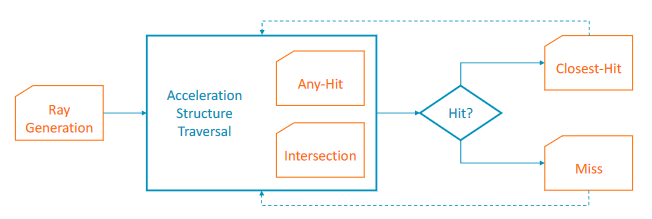
\includegraphics[width=0.7\linewidth]{Figures/full_rt_pap}
		\caption[Fluss-ähnliches Diagramm einer Raytracing-Pipeline]{Fluss-ähnliches Diagramm einer Raytracing-Pipeline\cite{Vulkanised2023}}
	\end{figure}
	
	Im Gegensatz dazu lagern Ray Queries diese Shader-Funktionalität auf den Anwender aus, der innerhalb des Shaders entscheidet, was bei einem Treffer oder Fehltreffer geschieht (Siehe Abbildung \ref{fig:rayquerypap}).
	
	\begin{figure}[h]
		\centering
		\label{fig:rayquerypap}
		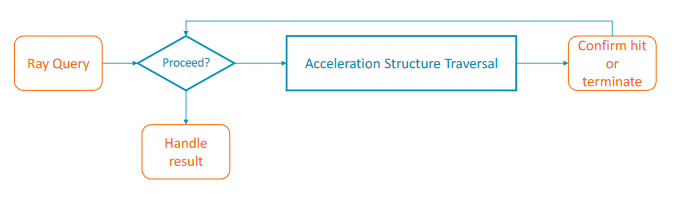
\includegraphics[width=0.7\linewidth]{Figures/rayquery_pap}
		\caption[Fluss-ähnliches Diagramm einer Ray Query]{Fluss-ähnliches Diagramm einer Ray Query\cite{Vulkanised2023}}
	\end{figure}
	
	Ein weiteres Merkmal von Raytracing-Pipelines ist das Abprallen von Strahlen, das typischerweise Photonen nachahmt, die von einer Lichtquelle emittiert werden. Bei Ray Queries kann dieses Verhalten durch den Anwender optional implementiert werden, spielt jedoch in dieser Arbeit keine Rolle.
	
	Neben den Strahlinformationen benötigen Ray Queries auch die Geometrie, gegen die der Strahl projiziert werden soll. RT-Kerne verwenden eine spezielle Darstellungsform von Geometrie, sogenannte Acceleration Structures.
	
	Acceleration Structures, die von Vulkan verwendet werden, bestehen aus zwei Komponenten: der Bottom-Level Acceleration Structure (BLAS) und der Top-Level Acceleration Structure (TLAS)\cite{VulkanAccelerationStructures}. Die BLAS enthält die tatsächliche Geometrie der 3D-Modelle der Szene. Die TLAS hingegen enthält Instanzen, also Transformationsinformationen eines 3D-Modells wie Position, Rotation und Skalierung. Eine häufige Optimierung in Game-Engines besteht darin, 3D-Modelle zu instanziieren, d. h., dieselbe Geometrie mehrmals mit unterschiedlichen Transformationsinformationen zu verwenden. Diese Instanzen referenzieren dieselben Geometriedaten, was dazu führt, dass die Geometrie nur einmal auf der GPU existieren muss, jedoch basierend auf den Instanzen mehrfach gerendert werden kann. Die TLAS ist eine Repräsentation dieser Instanzen, welche für die Nutzung durch Ray Queries optimiert ist. Abbildung \ref{fig:accelerationstructure} zeigt eine Visualisierung von BLAS und TLAS.
	
	\begin{figure}[h]
		\centering
		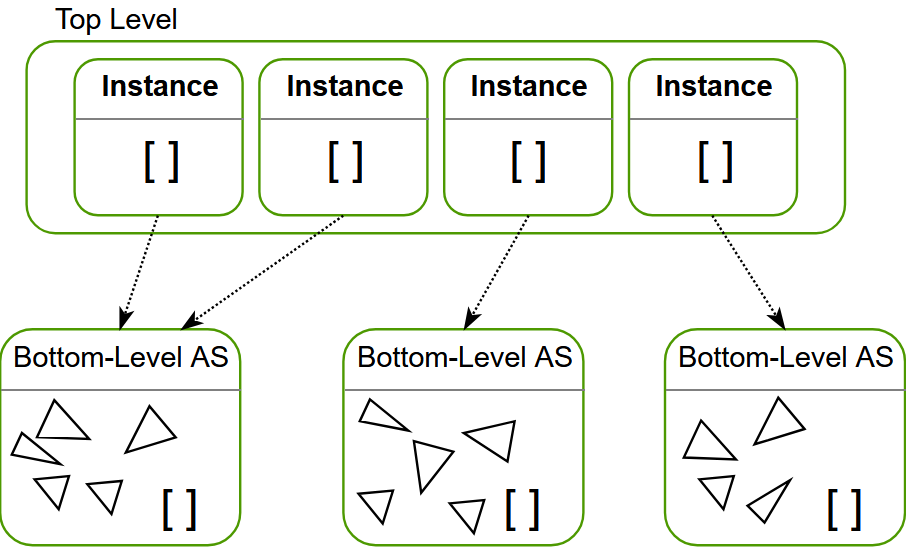
\includegraphics[width=0.7\linewidth]{Figures/acceleration_structures}
		\caption[Acceleration Structure]{Übersicht einer Acceleration Structure\cite{Bickford}}
		\label{fig:accelerationstructure}
	\end{figure}
	
	
	Moderne GPUs bieten eine Vielzahl von Shadern, darunter auch Compute-Shader. Compute-Shader sind universelle Werkzeuge, die es ermöglichen, Berechnungen hochparallelisiert auf der GPU durchzuführen, ohne dass diese Rendering-basiert sein müssen. Ray Queries können in solchen Compute-Shadern ausgeführt werden.
	
	Um die Acceleration Structures und die Strahlinformationen an die Ray Query weiterzugeben, wird ein Compute-Shader erstellt und mit den notwendigen Daten versorgt. Die Ray Query wird dann ausgeführt, und das Ergebnis wird an den Compute-Shader zurückgegeben. Dieser übermittelt das Ergebnis in Form eines booleschen Wahrheitswerts an die CPU und somit an den Aufrufer.
	
	Zum Messen der Performance beider Implementierungen wird eine einfache \textit{Stopwatch}-Klasse verwendet um die Zeit an zwei Punkten zu messen und voneinander subtrahieren. Die Differenz wird in Millisekunden angegeben.
	
	Als Referenzimplementierung dient die Unreal Engine 5. Diese Engine enthält die eigens entwickelte Physik-Engine \textit{Chaos} und repräsentiert den aktuellen Stand der Technik. Aufgrund ihrer weiten Verbreitung in der Videospielbranche eignet sie sich ideal für einen Vergleich.
	
	Um die beiden Ansätze vergleichen zu können, werden mehrere Testszenarien definiert, die aus einer variablen Anzahl von 3D-Modellen bestehen, die von Strahlen beschossen werden.

	Um sicherzustellen, dass die Szenarien in beiden Implementierungen identisch sind, wird ein CSV-Datenformat definiert. Jede Zeile entspricht einem 3D-Modell sowie dessen Position, Rotation und Skalierung, dem Strahltyp (einzeln oder kegelförmig), Strahlursprung und -richtung. Für jedes Szenario wird eine separate CSV-Datei erstellt. Die Implementierung lädt beim Start die entsprechende CSV-Datei, führt das Szenario automatisch aus und speichert die Messwerte ebenfalls in einer CSV-Datei ab. Die Auswertung der Messdaten erfolgt mithilfe von Microsoft Excel.
	
	Unreal Engine 5 bietet zudem die Möglichkeit die Treffererkennung basierend auf dem eigentlichen 3D-Modell durchzuführen anstatt mit Hitboxen. Daher werden die Testszenarien in der UE5 Implementation jeweils für Hitboxen sowie 3D-Modelle durchgeführt.
	
	Testszenarien werden in UE5 mithilfe von selbstgeschriebenen Skripten erstellt und in CSV-Dateien exportiert.
	
	
	\subsection{Zusammenfassung}
	
	In modernen Game-Engines erfolgt die Treffererkennung typischerweise durch eine Funktion, die Strahlen in die Szene projiziert und auf Kollisionen prüft. Diese Berechnungen werden meist auf der CPU durchgeführt und nutzen vereinfachte Hitboxen, was jedoch zu Ungenauigkeiten wie False-Negatives oder False-Positives führen kann. Diese Probleme sind besonders in kompetitiven Spielen relevant, da sie das Spielerlebnis beeinträchtigen und zusätzlichen Entwicklungsaufwand erfordern. Eine vielversprechende Alternative ist die Verlagerung der Berechnungen auf die GPU, insbesondere durch den Einsatz von Raytracing-Kernen und Ray Queries, wie sie von der Vulkan-API bereitgestellt werden. In dieser Arbeit wird die Funktion \textit{traceRay} auf der GPU implementiert, um die Leistung und Genauigkeit gegenüber einer CPU-basierten Referenzimplementierung in der Unreal Engine 5 zu vergleichen. Hierfür werden mehrere Testszenarien definiert, in denen die Berechnungszeiten der beiden Ansätze miteinander verglichen werden.
	
	\pagebreak
	\section{Prototypische Realisierung}
	
	Das Kapitel gliedert sich in zwei Bereiche. 

	Der erste Bereich behandelt die Implementierung des Konzepts innerhalb einer eigens entwickelten Prism Game-Engine und legt dabei den Schwerpunkt auf Vulkan-bezogene Themen. Hier werden spezifische technische Vulkan-Details und ihre Anwendung in der Engine beschrieben. Die Implementierung erfolgt mit dem offiziellen C++ Wrapper \textit{Vulkan-Hpp}\cite{VulkanHpp}.
	
	Der zweite und letzte Bereich konzentriert sich auf die CPU-basierte Implementierung des Konzepts in Unreal Engine 5. Dabei wird der Fokus auf die wesentlichen Unterschiede bei der Umsetzung gelegt.

	\subsection{Prism Engine-Implementation}

	Um die im Konzept angesprochene \textit{traceRay}-Funktion zu implementieren, bedarf es mehrerer Schritte zuvor. Vulkan besteht aus einer Kernkomponente \textit{Core} sowie optionale \textit{Extensions}. Fordert der Benutzer eine \textit{Extension} in Vulkan an, gibt der Grafiktreiber Rückmeldung ob diese implementiert ist und bereitgestellt werden kann. 
	Ray Queries in Vulkan sind eine solche \textit{Extension}. \textit{Extensions} müssen bei Initialisierung des Logical Device angefragt werden (Siehe Listings \ref{lst:listing-vulkan-extensionhpp}-\ref{lst:listing-vulkan-extensioncpp}). 
	
	\begin{lstlisting}[caption={Definition der Raytracing Extensions in VulkanRenderer.hpp},label={lst:listing-vulkan-extensionhpp}]
	...
	std::vector<const char*> deviceExtensions = {
		...
		VK_KHR_ACCELERATION_STRUCTURE_EXTENSION_NAME,
		...
		VK_KHR_RAY_QUERY_EXTENSION_NAME,
		VK_KHR_BUFFER_DEVICE_ADDRESS_EXTENSION_NAME
	};
	...\end{lstlisting}
	
	\begin{lstlisting}[caption={Anfragen der Raytracing Extensions in VulkanRenderer.cpp},label={lst:listing-vulkan-extensioncpp}]
	...
    vk::PhysicalDeviceFeatures deviceFeatures;
	...
	vk::PhysicalDeviceAccelerationStructureFeaturesKHR accelerationStructureFeatures;
	accelerationStructureFeatures.accelerationStructure = VK_TRUE;
	vk::PhysicalDeviceRayQueryFeaturesKHR rayQueryFeatures;
	rayQueryFeatures.rayQuery = VK_TRUE;
	rayQueryFeatures.pNext = &accelerationStructureFeatures;
	vk::PhysicalDeviceBufferDeviceAddressFeatures bufferDeviceAddressFeatures;
	bufferDeviceAddressFeatures.bufferDeviceAddress = VK_TRUE;
	bufferDeviceAddressFeatures.pNext = &rayQueryFeatures;
	auto createInfo = vk::DeviceCreateInfo(
	vk::DeviceCreateFlags(),
	static_cast<uint32_t>(queueCreateInfos.size()),
	queueCreateInfos.data()
	);
	createInfo.pEnabledFeatures = &deviceFeatures;
	createInfo.pNext = &bufferDeviceAddressFeatures;
	createInfo.enabledExtensionCount = static_cast<uint32_t>(deviceExtensions.size());
	createInfo.ppEnabledExtensionNames = deviceExtensions.data();
	...
	logicalDevice = physicalDevice.createDeviceUnique(createInfo);
	...\end{lstlisting}
	
	Als nächstes wird der Compute-Shader geladen. Zunächst definiert die Funktion \textit{createComputeDescriptorSetLayout} das Layout des Descriptor Sets für die Compute-Pipeline. Hierbei werden drei Binding} erstellt: eines für die TLAS, eines für den Eingabe-Storage-Buffer und eines für den Ausgabe-Storage-Buffer. Diese Bindings sind essentiell, um später die entsprechenden Ressourcen mit der Compute-Pipeline zu verknüpfen. Siehe dazu Listing \ref{lst:listing-vulkan-descriptorsetlayoutcpp}.
	
	\begin{lstlisting}[caption={Erzeugen des \textit{Descriptor Set Layouts} in VulkanRenderer.cpp},label={lst:listing-vulkan-descriptorsetlayoutcpp}]
void VulkanRenderer::createComputeDescriptorSetLayout()
{
	vk::DescriptorSetLayoutBinding tlasLayoutBinding;
	tlasLayoutBinding.binding = 0;
	tlasLayoutBinding.descriptorType = vk::DescriptorType::eAccelerationStructureKHR;
	tlasLayoutBinding.descriptorCount = 1;
	tlasLayoutBinding.stageFlags = vk::ShaderStageFlagBits::eCompute;
	tlasLayoutBinding.pImmutableSamplers = nullptr;
	vk::DescriptorSetLayoutBinding inputStorageBufferLayoutBinding;
	inputStorageBufferLayoutBinding.binding = 1;
	inputStorageBufferLayoutBinding.descriptorType = vk::DescriptorType::eStorageBuffer;
	inputStorageBufferLayoutBinding.descriptorCount = 1;
	inputStorageBufferLayoutBinding.stageFlags = vk::ShaderStageFlagBits::eCompute;
	inputStorageBufferLayoutBinding.pImmutableSamplers = nullptr;
	vk::DescriptorSetLayoutBinding outputStorageBufferLayoutBinding;
	outputStorageBufferLayoutBinding.binding = 2;
	outputStorageBufferLayoutBinding.descriptorType = vk::DescriptorType::eStorageBuffer;
	outputStorageBufferLayoutBinding.descriptorCount = 1;
	outputStorageBufferLayoutBinding.stageFlags = vk::ShaderStageFlagBits::eCompute;
	outputStorageBufferLayoutBinding.pImmutableSamplers = nullptr;
	const std::array bindings = {
		tlasLayoutBinding, inputStorageBufferLayoutBinding, outputStorageBufferLayoutBinding
	};
	vk::DescriptorSetLayoutCreateInfo layoutInfo = {};
	layoutInfo.bindingCount = static_cast<uint32_t>(bindings.size());
	layoutInfo.pBindings = bindings.data();
	...
	computeDescriptorSetLayout = logicalDevice->createDescriptorSetLayout(layoutInfo);
	...
}	\end{lstlisting}
	
	Im nächsten Schritt wird in der Funktion \textit{createComputePipeline} die Compute-Pipeline selbst erstellt. Dazu wird zunächst das SPIR-V Shader-Modul für den Compute-Shader geladen und konfiguriert. Anschließend erfolgt die Erstellung des Pipeline-Layouts, das dass zuvor definierte Descriptor Set Layout einbezieht. Danach wird die Compute-Pipeline aufgebaut und entsprechend konfiguriert, um für die Berechnungen bereit zu sein. Siehe dazu Listing \ref{lst:listing-vulkan-computepipelinecpp} im Anhang.
	
	Daraufhin erstellt die Funktion \textit{createComputeStorageBuffers} die Buffer, die innerhalb der Compute-Pipeline verwendet werden (Siehe Listing \ref{lst:listing-vulkan-computestoragebufferscpp}). Es werden sowohl ein Eingabebuffer als auch ein Ausgabebuffer angelegt. 
	
	\begin{lstlisting}[caption={Erstellen der Shader Storage Buffer Objects in VulkanRenderer.cpp},label={lst:listing-vulkan-computestoragebufferscpp}]
void VulkanRenderer::createComputeStorageBuffers()
{
	constexpr auto inputBufferSize = sizeof(ComputeInputBufferObject);
	createBuffer(inputBufferSize, vk::BufferUsageFlagBits::eStorageBuffer,
	vk::MemoryPropertyFlagBits::eHostVisible |
	vk::MemoryPropertyFlagBits::eHostCoherent, inputComputeBuffer, inputComputeBufferMemory);
	constexpr auto outputBufferSize = sizeof(ComputeOutputBufferObject);
	createBuffer(outputBufferSize, vk::BufferUsageFlagBits::eStorageBuffer,
	vk::MemoryPropertyFlagBits::eHostVisible |
	vk::MemoryPropertyFlagBits::eHostCoherent, outputComputeBuffer, outputComputeBufferMemory);
}	\end{lstlisting}
	
	Die \textit{Memory Flags}, die in dieser Funktion verwendet werden, sind \textit{eHostVisible} und\textit{eHostCoherent}. Sie definieren wichtige Eigenschaften des zugewiesenen Speichers:
	\begin{itemize}
		\item \textbf{vk::MemoryPropertyFlagBits::eHostVisible}: Dieses Flag stellt sicher, dass der Speicherbereich von der CPU aus sichtbar ist, was bedeutet, dass die CPU direkt auf den Speicher zugreifen und Daten lesen oder schreiben kann. Dies ist notwendig, um Daten in den Buffer zu laden (im Fall des \textit{Eingabebuffers}) oder um Ergebnisse aus dem Buffer auszulesen (im Fall des Ausgabebuffers).\cite{VulkanMemoryFlags}
		\item \textbf{vk::MemoryPropertyFlagBits::eHostCoherent}: Dieses Flag garantiert, dass Änderungen am Speicherbereich sofort für beide Seiten – sowohl die CPU als auch die GPU – sichtbar sind. Ohne dieses Flag müsste man explizit Speicherbereiche \textit{flushen} (d.h. sicherstellen, dass alle Änderungen von der CPU zur GPU übertragen werden) oder \textit{invalidate} (d.h. sicherstellen, dass die CPU die aktuellen Daten von der GPU sieht). Mit \textit{eHostCoherent} entfällt dieser zusätzliche Aufwand, da die Kohärenz zwischen Host- und Device-Memory automatisch gewährleistet ist.\cite{VulkanMemoryFlags}
	\end{itemize}

	Beide Buffer werden zudem mit der Größe der Structs ComputeInputBufferObject (Anhang, Listing \ref{lst:listing-vulkan-computeinputbuffer}) und \textit{ComputeOutputBufferObject} (Anhang, Listing \ref{lst:listing-vulkan-computeoutputbuffer}) erzeugt. Beide Shader Storage Buffer Objects geben das Speicher-Layout bzw. Speichergröße für Vulkan vor.
	
	Anschließend wird in der Funktion \textit{createComputeDescriptorPool} ein Descriptor Pool erstellt, aus dem die Descriptor Sets für die Compute-Pipeline allokiert werden. Dieser Pool beinhaltet Ressourcen für die TLAS und SSBOs. Siehe dazu Listing \ref{lst:listing-vulkan-computedescriptorpoolcpp} im Anhang.
	
	Die Funktion \textit{createComputeDescriptorSet} allokiert daraufhin das Descriptor Set aus dem zuvor erstellten Pool und befüllt es mit den erforderlichen Informationen, darunter der TLAS und die SSBOs. Diese Descriptor Sets sind für die Compute-Pipeline unerlässlich, da sie den Zugriff auf die entsprechenden Daten während der Ausführung der Raytracing-Berechnungen ermöglichen. Siehe dazu im Anhang Listing \ref{lst:listing-vulkan-computedescriptorsetcpp}.

	
	Zuletzt erstellt die Funktion \textit{createComputeCommandPool} einen Command Pool, der für die Compute-Pipeline verwendet wird. Dieser Pool dient der Allokation von Command Buffers, welche die Ausführung der Compute-Operationen auf der GPU steuern. Zusammengefasst sorgen diese Funktionen dafür, dass die grundlegenden Elemente einer Compute-Pipeline in Vulkan eingerichtet werden, wodurch die Durchführung von Raytracing-Berechnungen auf der GPU ermöglicht wird. Siehe Listing \ref{lst:listing-vulkan-computecommandpoolcpp} im Anhang.
	
	Nun sind alle Vorraussetzungen für das Ausführen des Compute-Shaders erfüllt. Bevor jedoch die eigentliche \textit{traceRay} Funktion implementiert werden kann, bedarf es der Erzeugung der BLAS und TLAS.
	
	Die \textit{Bottom-Level Acceleration-Structures} werden auf Basis der für Treffererkennung relevanten 3D-Modelldaten erzeugt (Siehe Listing \ref{lst:listing-vulkan-createblascpp}). Zu diesem Zweck müssen diese Daten zuerst in ein Zwischenformat gespeichert werden. Dies erledigt die \textit{collectAccelerationStructureGeometries} Funktion in Listing \ref{lst:listing-vulkan-collectiongeocpp}.
	
	\begin{lstlisting}[caption={Sammeln der 3D-Modellgeometrie in VulkanRenderer.cpp},label={lst:listing-vulkan-collectiongeocpp}]
std::vector<BottomLevelAccelerationStructureInput> VulkanRenderer::collectAccelerationStructureGeometries() const
{
	std::vector<BottomLevelAccelerationStructureInput> blasInputs;
	...
	for (const auto& vulkanMesh : meshes)
	{
		const auto meshAsset = assetManager->getAsset<Assets::StaticMeshAsset>(vulkanMesh->getMeshAssetName());
		...
		vk::AccelerationStructureGeometryTrianglesDataKHR triangleData;
		triangleData.vertexFormat = vk::Format::eR32G32B32Sfloat;
		triangleData.vertexData = getBufferDeviceAddress(vulkanMesh->getVertexBuffer().getBuffer());
		triangleData.vertexStride = sizeof(Vertex);
		triangleData.maxVertex = static_cast<uint32_t>(meshAsset->getVertices().size()) - 1;
		triangleData.indexType = vk::IndexType::eUint32;
		triangleData.indexData = getBufferDeviceAddress(vulkanMesh->getIndexBuffer().getBuffer());
		triangleData.transformData = nullptr;
		vk::AccelerationStructureGeometryKHR geometry;
		geometry.setGeometryType(vk::GeometryTypeKHR::eTriangles);
		geometry.setFlags(vk::GeometryFlagBitsKHR::eOpaque);
		geometry.geometry.setTriangles(triangleData);
		const uint32_t primitiveCount = static_cast<uint32_t>(meshAsset->getIndices().size() / 3);
		vk::AccelerationStructureBuildRangeInfoKHR buildRangeInfo;
		buildRangeInfo.setPrimitiveCount(primitiveCount);
		buildRangeInfo.setPrimitiveOffset(0);
		buildRangeInfo.setFirstVertex(0);
		buildRangeInfo.setTransformOffset(0);
		BottomLevelAccelerationStructureInput blasInput;
		blasInput.geometry = geometry;
		blasInput.rangeInfo = buildRangeInfo;
		blasInput.meshInstanceIds = vulkanMesh->getMeshIds();
		blasInputs.emplace_back(blasInput);
	}
	return blasInputs;
}	\end{lstlisting}
	
	Anschließend werden die Speicheranforderungen für jede BLAS berechnet, um die notwendige Größe für den temporären Speicher (Scratch Buffer) zu ermitteln, der während des Aufbaus benötigt wird.
	
	Sobald die benötigten Speichergrößen feststehen, wird ein Scratch Buffer erstellt, um den Aufbau der BLAS zu unterstützen. Daraufhin werden für jede gesammelte Geometrie leere BLAS-Strukturen im GPU-Speicher reserviert. Der eigentliche Aufbau der BLAS erfolgt durch das Laden der Geometrien in diese Strukturen. Hierfür wird ein Command Buffer verwendet, um die entsprechenden Operationen auf der GPU auszuführen. Nach der Ausführung des Command Buffers wird der Scratch Buffer wieder freigegeben, um somit den belegten Speicherplatz zu räumen. Abschließend werden die erstellten BLAS zurückgegeben, die dann für die Erzeugung der TLAS verwendet werden können.
	
	Relevant ist hierbei das Flag \textit{ePreferFastTrace}. Alternativ zu diesem gibt es unter anderem \textit{ePreferFastBuild}. Dies signalisiert Vulkan entweder die Optimierung der BLAS für schnelleres Raytracing oder schnelleres Erstellen der BLAS, jeweils zum Nachteil des anderen. Ebenfalls wichtig ist der \textit{BLAS build mode eBuild}. Anstatt die BLAS komplett neu zu erzeugen kann man diese auch updaten falls sich nur geringfügige Änderungen seit der letzten BLAS Erstellung ergeben haben.
	
	\begin{lstlisting}[caption={Erzeugung der Bottom-Level Acceleration Structures in VulkanRenderer.cpp},label={lst:listing-vulkan-createblascpp}]
std::vector<AccelerationStructure> VulkanRenderer::buildBottomLevelAccelerationStructures()
{
	...
	auto blasInputs = collectAccelerationStructureGeometries();
	...
	vk::DeviceSize totalAccelStructureSizeBytes = 0;
	vk::DeviceSize maxScratchSizeBytes = 0;
	std::vector<BuildAccelerationStructure> buildAccelerationStructures;
	buildAccelerationStructures.reserve(blasInputs.size());
	...
	for (auto& [geometry, rangeInfo, meshInstanceIds] : blasInputs)
	{
		vk::AccelerationStructureBuildGeometryInfoKHR buildGeometryInfo{};
		buildGeometryInfo.type = vk::AccelerationStructureTypeKHR::eBottomLevel;
		buildGeometryInfo.flags = vk::BuildAccelerationStructureFlagBitsKHR::ePreferFastTrace;
		buildGeometryInfo.mode = vk::BuildAccelerationStructureModeKHR::eBuild;
		buildGeometryInfo.geometryCount = 1;
		buildGeometryInfo.pGeometries = &geometry;
		vk::AccelerationStructureBuildSizesInfoKHR sizeInfo{};
		logicalDevice->getAccelerationStructureBuildSizesKHR(
		vk::AccelerationStructureBuildTypeKHR::eDevice,
		&buildGeometryInfo,
		&rangeInfo.primitiveCount,
		&sizeInfo
		);
		BuildAccelerationStructure buildAccelerationStructure{
			buildGeometryInfo, sizeInfo, rangeInfo, {{}, {}, {}, meshInstanceIds}
		};
		buildAccelerationStructures.emplace_back(buildAccelerationStructure);
		totalAccelStructureSizeBytes += sizeInfo.accelerationStructureSize;
		maxScratchSizeBytes = std::max(maxScratchSizeBytes, sizeInfo.buildScratchSize);
	}
	...
	vk::Buffer scratchBuffer;
	vk::DeviceMemory scratchBufferMemory;
	createBuffer(maxScratchSizeBytes,
	vk::BufferUsageFlagBits::eShaderDeviceAddress | vk::BufferUsageFlagBits::eStorageBuffer,
	vk::MemoryPropertyFlagBits::eDeviceLocal, scratchBuffer, scratchBufferMemory);
	vk::DeviceAddress scratchAddress = getBufferDeviceAddress(scratchBuffer);
	std::vector<vk::AccelerationStructureBuildGeometryInfoKHR> buildGeometryInfos;
	buildGeometryInfos.reserve(buildAccelerationStructures.size());
	std::vector<vk::AccelerationStructureBuildRangeInfoKHR> buildRangeInfos;
	buildRangeInfos.reserve(buildAccelerationStructures.size());
	std::vector<AccelerationStructure> blases;
	blases.reserve(buildAccelerationStructures.size());
	...
	for (auto& [buildInfo, buildSizesInfo, rangeInfo, accelerationStructure] : buildAccelerationStructures)
	{
		vk::AccelerationStructureCreateInfoKHR createInfo{};
		createInfo.type = vk::AccelerationStructureTypeKHR::eBottomLevel;
		createInfo.size = buildSizesInfo.accelerationStructureSize;
		createBuffer(createInfo.size,
		vk::BufferUsageFlagBits::eAccelerationStructureStorageKHR |
		vk::BufferUsageFlagBits::eShaderDeviceAddress, vk::MemoryPropertyFlagBits::eDeviceLocal,
		accelerationStructure.buffer,
		accelerationStructure.memory);
		createInfo.buffer = accelerationStructure.buffer;
		...
		accelerationStructure.accelerationStructureKHR = logicalDevice->createAccelerationStructureKHR(createInfo);
		...
		buildInfo.dstAccelerationStructure = accelerationStructure.
		accelerationStructureKHR;
		buildInfo.scratchData.deviceAddress = scratchAddress;
		buildGeometryInfos.emplace_back(buildInfo);
		buildRangeInfos.emplace_back(rangeInfo);
		blases.emplace_back(accelerationStructure);
	}
	...
	logicalDevice->resetCommandPool(computeCommandPool);
	vk::CommandBufferAllocateInfo allocInfo = {};
	allocInfo.level = vk::CommandBufferLevel::ePrimary;
	allocInfo.commandPool = computeCommandPool;
	allocInfo.commandBufferCount = 1;
	vk::CommandBuffer commandBuffer;
	...
	commandBuffer = logicalDevice->allocateCommandBuffers(allocInfo)[0];
	...
	vk::CommandBufferBeginInfo beginInfo = {};
	beginInfo.flags = vk::CommandBufferUsageFlagBits::eOneTimeSubmit;
	commandBuffer.begin(beginInfo);
	commandBuffer.buildAccelerationStructuresKHR(buildGeometryInfos, buildRangeInfos.data());
	commandBuffer.end();
	vk::SubmitInfo submitInfo = {};
	submitInfo.commandBufferCount = 1;
	submitInfo.pCommandBuffers = &commandBuffer;
	computeQueue.submit(submitInfo, nullptr);
	computeQueue.waitIdle();
	...
	logicalDevice->destroyBuffer(scratchBuffer);
	logicalDevice->freeMemory(scratchBufferMemory);
	...
	return blases;
}	\end{lstlisting}
	
	Die Top-Level Acceleration Structure dient als übergeordnete Datenstruktur, die Referenzen auf mehrere BLAS enthält, wodurch eine hierarchische Organisation der Szenengeometrien ermöglicht wird.
	
	Der Prozess beginnt mit der Erstellung einer Liste von Instanzen, wobei jede Instanz eine Referenz auf genau eine BLAS darstellt. Jede Instanz-TLAS enthält unter anderem die Transformationsmatrix der 3D-Modellinstanz sowie die Speicheradresse der BLAS.
	
	Im nächsten Schritt wird ein Command Buffer initialisiert, der zur Ausführung der notwendigen GPU-Operationen dient. Es wird ein temporärer Staging Buffer erstellt, in dem die Instanzen vorübergehend im Host-Speicher abgelegt werden. Dieser Staging Buffer wird dann in einen Buffer auf der GPU kopiert, der die Instanzen für den weiteren Aufbau der TLAS bereitstellt.
	
	Nachdem die Instanzen in den GPU-Speicher kopiert wurden, wird eine Memory Barrier gesetzt, um sicherzustellen, dass alle Speicheroperationen abgeschlossen sind, bevor die TLAS aufgebaut wird. Die Funktion berechnet dann die notwendigen Speichergrößen für die TLAS und allokiert den benötigten Speicher auf der GPU. Zusätzlich wird ein Scratch Buffer erstellt, der temporär für den Aufbau der TLAS verwendet wird.
	
	Schließlich werden die TLAS durch einen Aufruf des Command Buffers aufgebaut, der die Instanzen verarbeitet und die TLAS erstellt. Nach Abschluss des Aufbaus wird der Command Buffer beendet, und die GPU führt die entsprechenden Operationen aus. Nachdem der Aufbau abgeschlossen ist, wird auf das Beenden der GPU-Operationen gewartet, und die temporären Buffer werden freigegeben. Siehe dazu Listing \ref{lst:listing-vulkan-createtlascpp}.
	
	\begin{lstlisting}[caption={Erzeugung der Top-Level Acceleration Structure in VulkanRenderer.cpp},label={lst:listing-vulkan-createtlascpp}]
AccelerationStructure VulkanRenderer::buildTopLevelAccelerationStructure(
const std::vector<AccelerationStructure>& blases)
{
	std::vector<vk::AccelerationStructureInstanceKHR> instances;
	instances.reserve(blases.size());
	const auto activeScene = sceneManager->getActiveScene();
	const auto staticMeshComponents = activeScene->getComponents<Core::StaticMeshComponent>();
	for (const auto& blas : blases)
	{
		auto matchingComponents = staticMeshComponents
		| std::views::filter([&](const auto& staticMeshComponent)
		{
			auto meshId = staticMeshComponent->getStaticMesh()->getMeshId();
			return std::ranges::any_of(blas.meshInstanceIds, [&](const auto& instanceId)
			{
				return instanceId == meshId && staticMeshComponent->isCollidable();
			});
		});
		for (auto staticMeshComponent : matchingComponents)
		{
			vk::AccelerationStructureInstanceKHR asInstance{};
			asInstance.transform = glmMat4ToVkTransformMatrix(
			staticMeshComponent->getAbsoluteTransform().toMatrix());
			asInstance.instanceCustomIndex = 0;
			asInstance.accelerationStructureReference = getBlasBufferAddress(blas);
			asInstance.setFlags(vk::GeometryInstanceFlagBitsKHR::eTriangleCullDisable);
			asInstance.mask = 0xFF;
			asInstance.instanceShaderBindingTableRecordOffset = 0;
			instances.emplace_back(asInstance);
		}
	}
	const auto instanceCount = static_cast<uint32_t>(instances.size());
	logicalDevice->resetCommandPool(computeCommandPool);
	vk::CommandBufferAllocateInfo allocInfo = {};
	allocInfo.level = vk::CommandBufferLevel::ePrimary;
	allocInfo.commandPool = computeCommandPool;
	allocInfo.commandBufferCount = 1;
	vk::CommandBuffer commandBuffer;
	...
	commandBuffer = logicalDevice->allocateCommandBuffers(allocInfo)[0];
	...
	vk::CommandBufferBeginInfo beginInfo = {};
	beginInfo.flags = vk::CommandBufferUsageFlagBits::eOneTimeSubmit;
	commandBuffer.begin(beginInfo);
	vk::Buffer instanceStagingBuffer;
	vk::DeviceMemory instanceStagingBufferMemory;
	const auto stagingBufferSize = instances.size() * sizeof(vk::AccelerationStructureInstanceKHR);
	createBuffer(stagingBufferSize, vk::BufferUsageFlagBits::eTransferSrc,
	vk::MemoryPropertyFlagBits::eHostVisible | vk::MemoryPropertyFlagBits::eHostCoherent,
	instanceStagingBuffer, instanceStagingBufferMemory);
	void* data = logicalDevice->mapMemory(instanceStagingBufferMemory, 0, stagingBufferSize);
	memcpy(data, instances.data(), stagingBufferSize);
	logicalDevice->unmapMemory(instanceStagingBufferMemory);
	vk::Buffer instanceBuffer;
	vk::DeviceMemory instanceBufferMemory;
	createBuffer(stagingBufferSize,
	vk::BufferUsageFlagBits::eShaderDeviceAddress |
	vk::BufferUsageFlagBits::eAccelerationStructureBuildInputReadOnlyKHR |
	vk::BufferUsageFlagBits::eTransferDst,
	vk::MemoryPropertyFlagBits::eDeviceLocal,
	instanceBuffer, instanceBufferMemory);
	copyBuffer(instanceStagingBuffer, instanceBuffer, stagingBufferSize, commandBuffer);
	vk::BufferMemoryBarrier instanceBufferMemoryBarrier{};
	instanceBufferMemoryBarrier.srcAccessMask = vk::AccessFlagBits::eTransferWrite;
	instanceBufferMemoryBarrier.dstAccessMask = vk::AccessFlagBits::eAccelerationStructureWriteKHR;
	instanceBufferMemoryBarrier.srcQueueFamilyIndex = VK_QUEUE_FAMILY_IGNORED;
	instanceBufferMemoryBarrier.dstQueueFamilyIndex = VK_QUEUE_FAMILY_IGNORED;
	instanceBufferMemoryBarrier.buffer = instanceBuffer;
	instanceBufferMemoryBarrier.size = stagingBufferSize;
	vk::PipelineStageFlags srcStageMask = vk::PipelineStageFlagBits::eTransfer;
	vk::PipelineStageFlags dstStageMask = vk::PipelineStageFlagBits::eAccelerationStructureBuildKHR;
	vk::DependencyFlags dependencyFlags = {};
	commandBuffer.pipelineBarrier(srcStageMask, dstStageMask, dependencyFlags, nullptr, instanceBufferMemoryBarrier,
	nullptr);
	auto instanceBufferAddress = getBufferDeviceAddress(instanceBuffer);
	vk::AccelerationStructureGeometryInstancesDataKHR instancesData{};
	instancesData.data.deviceAddress = instanceBufferAddress;
	const vk::AccelerationStructureGeometryKHR tlasGeometry{vk::GeometryTypeKHR::eInstances, instancesData};
	vk::AccelerationStructureBuildGeometryInfoKHR buildGeometryInfo{};
	buildGeometryInfo.flags = vk::BuildAccelerationStructureFlagBitsKHR::ePreferFastTrace;
	buildGeometryInfo.geometryCount = 1;
	buildGeometryInfo.pGeometries = &tlasGeometry;
	buildGeometryInfo.mode = vk::BuildAccelerationStructureModeKHR::eBuild;
	buildGeometryInfo.type = vk::AccelerationStructureTypeKHR::eTopLevel;
	buildGeometryInfo.srcAccelerationStructure = nullptr;
	vk::AccelerationStructureBuildSizesInfoKHR buildSizesInfo{};
	logicalDevice->getAccelerationStructureBuildSizesKHR(
	vk::AccelerationStructureBuildTypeKHR::eDevice,
	&buildGeometryInfo,
	&instanceCount,
	&buildSizesInfo
	);
	vk::AccelerationStructureCreateInfoKHR createInfo{};
	createInfo.size = buildSizesInfo.accelerationStructureSize;
	createInfo.type = vk::AccelerationStructureTypeKHR::eTopLevel;
	AccelerationStructure tlas;
	createBuffer(createInfo.size,
	vk::BufferUsageFlagBits::eAccelerationStructureStorageKHR |
	vk::BufferUsageFlagBits::eShaderDeviceAddress, vk::MemoryPropertyFlagBits::eDeviceLocal,
	tlas.buffer, tlas.memory);
	createInfo.buffer = tlas.buffer;
	tlas.accelerationStructureKHR = logicalDevice->createAccelerationStructureKHR(createInfo);
	vk::Buffer scratchBuffer;
	vk::DeviceMemory scratchBufferMemory;
	createBuffer(buildSizesInfo.buildScratchSize,
	vk::BufferUsageFlagBits::eStorageBuffer | vk::BufferUsageFlagBits::eShaderDeviceAddress,
	vk::MemoryPropertyFlagBits::eDeviceLocal, scratchBuffer, scratchBufferMemory);
	const auto scratchBufferAddress = getBufferDeviceAddress(scratchBuffer);
	buildGeometryInfo.dstAccelerationStructure = tlas.accelerationStructureKHR;
	buildGeometryInfo.scratchData.deviceAddress = scratchBufferAddress;
	vk::AccelerationStructureBuildRangeInfoKHR buildRangeInfo{instanceCount, 0, 0, 0};
	commandBuffer.buildAccelerationStructuresKHR({buildGeometryInfo}, &buildRangeInfo);
	commandBuffer.end();
	vk::SubmitInfo submitInfo = {};
	submitInfo.commandBufferCount = 1;
	submitInfo.pCommandBuffers = &commandBuffer;
	computeQueue.submit(submitInfo, nullptr);
	// Wait for compute queue to finish
	computeQueue.waitIdle();
	logicalDevice->destroyBuffer(scratchBuffer);
	logicalDevice->freeMemory(scratchBufferMemory);
	logicalDevice->destroyBuffer(instanceStagingBuffer);
	logicalDevice->freeMemory(instanceStagingBufferMemory);
	logicalDevice->destroyBuffer(instanceBuffer);
	logicalDevice->freeMemory(instanceBufferMemory);
	...
	return tlas;
}	\end{lstlisting}
	
	Die Funktion \textit{traceRays} in Listing \ref{lst:listing-vulkan-traceraycpp} dient der Durchführung der Raytracing-Operation innerhalb einer Vulkan-basierten Pipeline. Sie nimmt als Eingabe eine Liste an Structs, bestehend aus dem Strahlursprung, der Richtung eines Strahls sowie minimale und maximale Länge für die Strahlverfolgung. Der Hauptzweck dieser Funktion besteht darin, festzustellen, ob die gegebenen Strahlen ein Objekt in der Szene trifft.
	
	Zu Beginn der Funktion wird eine Bereinigung der vorherigen Raytracing-Daten durchgeführt, um sicherzustellen, dass keine veralteten Informationen den aktuellen Prozess beeinflussen.
	
	Der nächste Schritt umfasst den Aufbau der notwendigen Beschleunigungsstrukturen. Zunächst werden die BLAS durch Aufrufen der zuvor beschriebenen Funktion \textit{buildBottomLevelAccelerationStructures} erstellt. Diese Strukturen repräsentieren die grundlegenden geometrischen Daten der Szene. Daraufhin werden die TLAS mit der ebenfalls beschriebenen Funktion \textit{buildTopLevelAccelerationStructure} generiert, welche die BLAS referenziert und eine hierarchische Organisation der Szene ermöglicht.
	
	Anschließend werden SSBOs erstellt und mit den Parametern der Strahlen befüllt. Falls der Aufrufer mehr Strahlen projizieren will als der SSBO-Speicher fassen kann, wird dieser vergrößert.
	
	Nachdem die Beschleunigungsstrukturen erstellt wurden und die SSBOs befüllt sind, wird das Descriptor Set für die Compute-Pipeline aktualisiert, um die TLAS und ggf. die neuen SSBOs einzubinden. Dies ermöglicht es der GPU, während der Raytracing-Operation effizient auf die Szenendaten zuzugreifen. Zudem werden die SSBOs in den Grafikspeicher kopiert, sodass der Compute-Shader auf die Daten zugreifen kann.
	
	Ein Command Buffer wird initialisiert und konfiguriert, um die Compute-Pipeline auszuführen. Innerhalb dieses Buffers wird der entsprechende Compute-Shader gebunden, der für die Raytracing-Operation verantwortlich ist. Um von möglichst von der Multithreading-Fähigkeit der Grafikkarte zu profitieren wird auf Basis der Anzahl der zu projizierenden Strahlen die Anzahl der \textit{Work Groups}, also der Arbeitspakete die auf den Compute Units\footnote{Prozessoren zur Verarbeitung von Compute Shadern} der GPU verarbeit werden, definiert. Eine \textit{Work Group} besteht aus 16 \textit{Work Items}, welche jeweils einen Shader-Aufruf darstellen.
	
	Durch den Aufruf von \textit{dispatch} werden die \textit{Work Groups} ausgeführt.
	
	Nach der Ausführung des Command Buffers und dem Abschluss aller GPU-Operationen werden die Ergebnisse aus dem GPU-Speicher zurück in den Host-Speicher übertragen. Die Ausgabe-SSBOs werden ausgelesen, um festzustellen, ob die Strahlen ein Objekt getroffen haben. Die Ergebnisse werden anschließend an den Funktionsaufrufer zurückgegeben.
	
	\begin{lstlisting}[caption={\textit{traceRay} Funktion in VulkanRenderer.cpp},label={lst:listing-vulkan-traceraycpp}]
std::vector<HitDetection::RayHitInfo> VulkanRenderer::traceRays(const std::vector<HitDetection::RayInfo>& rayInfos)
{
	std::vector<HitDetection::RayHitInfo> results;
	results.reserve(rayInfos.size());
	...
	cleanupRaytracingData();
	...
	bottomLevelAccelerationStructures = buildBottomLevelAccelerationStructures();
	...
	topLevelAccelerationStructure = buildTopLevelAccelerationStructure(bottomLevelAccelerationStructures);
	...
	const vk::WriteDescriptorSetAccelerationStructureKHR tlasDescriptorWrite{
		1, &topLevelAccelerationStructure.accelerationStructureKHR
	};
	
	// update compute input buffer
	std::vector<HitDetection::ComputeInputBufferObject> inputBufferObjects;
	inputBufferObjects.reserve(rayInfos.size());
	for (size_t i = 0; i < rayInfos.size(); ++i)
	{
		const auto& rayInfo = rayInfos[i];
		auto rayOriginInverted = rayInfo.getOrigin();
		rayOriginInverted.y = -rayOriginInverted.y; // Invert Y axis for Vulkan
		inputBufferObjects.emplace_back(rayOriginInverted, rayInfo.getDirection(), rayInfo.getMinDistance(),
		rayInfo.getMaxDistance(), i);
	}
	...
	// If necessary, recreate the compute storage buffers
	createComputeStorageBuffers(inputBufferObjects.size(), rayInfos.size(), false);
	// We have a new TLAS so we need the descriptorset to know about it. Otherwise the old one will be used again.
	vk::WriteDescriptorSet accelerationStructureDescriptorWrite{};
	accelerationStructureDescriptorWrite.dstSet = computeDescriptorSet;
	accelerationStructureDescriptorWrite.dstBinding = 0;
	accelerationStructureDescriptorWrite.dstArrayElement = 0;
	accelerationStructureDescriptorWrite.descriptorType = vk::DescriptorType::eAccelerationStructureKHR;
	accelerationStructureDescriptorWrite.descriptorCount = 1;
	accelerationStructureDescriptorWrite.pNext = &tlasDescriptorWrite;
	const vk::DescriptorBufferInfo inputBufferInfo{inputComputeBuffer, 0, sizeof(HitDetection::ComputeInputBufferObject)};
	vk::WriteDescriptorSet inputDescriptorWrite = {};
	inputDescriptorWrite.dstSet = computeDescriptorSet;
	inputDescriptorWrite.dstBinding = 1;
	inputDescriptorWrite.dstArrayElement = 0;
	inputDescriptorWrite.descriptorType = vk::DescriptorType::eStorageBuffer;
	inputDescriptorWrite.descriptorCount = 1;
	inputDescriptorWrite.pBufferInfo = &inputBufferInfo;
	const vk::DescriptorBufferInfo outputBufferInfo{outputComputeBuffer, 0, sizeof(HitDetection::ComputeOutputBufferObject)};
	vk::WriteDescriptorSet outputDescriptorWrite = {};
	outputDescriptorWrite.dstSet = computeDescriptorSet;
	outputDescriptorWrite.dstBinding = 2;
	outputDescriptorWrite.dstArrayElement = 0;
	outputDescriptorWrite.descriptorType = vk::DescriptorType::eStorageBuffer;
	outputDescriptorWrite.descriptorCount = 1;
	outputDescriptorWrite.pBufferInfo = &outputBufferInfo;
	logicalDevice->updateDescriptorSets({
		accelerationStructureDescriptorWrite, inputDescriptorWrite,
		outputDescriptorWrite
	}, nullptr);
	const vk::DeviceSize bufferSize = sizeof(HitDetection::ComputeInputBufferObject) * inputBufferObjects.size();
	void* data = logicalDevice->mapMemory(inputComputeBufferMemory, 0, bufferSize);
	memcpy(data, inputBufferObjects.data(), bufferSize);
	logicalDevice->unmapMemory(inputComputeBufferMemory);
	...
	logicalDevice->resetCommandPool(computeCommandPool);
	vk::CommandBufferAllocateInfo allocInfo = {};
	allocInfo.level = vk::CommandBufferLevel::ePrimary;
	allocInfo.commandPool = computeCommandPool;
	allocInfo.commandBufferCount = 1;
	vk::CommandBuffer commandBuffer;
	...
	commandBuffer = logicalDevice->allocateCommandBuffers(allocInfo)[0];
	...
	vk::CommandBufferBeginInfo beginInfo = {};
	beginInfo.flags = vk::CommandBufferUsageFlagBits::eOneTimeSubmit;
	commandBuffer.begin(beginInfo);
	commandBuffer.bindPipeline(vk::PipelineBindPoint::eCompute, computePipeline);
	commandBuffer.bindDescriptorSets(vk::PipelineBindPoint::eCompute, computePipelineLayout, 0, 1,
	&computeDescriptorSet, 0, nullptr);
	uint32_t workgroupCountX = (rayInfos.size() + 15) / 16;
	commandBuffer.dispatch(workgroupCountX, 1, 1);
	commandBuffer.end();
	...
	vk::SubmitInfo submitInfo = {};
	submitInfo.commandBufferCount = 1;
	submitInfo.pCommandBuffers = &commandBuffer;
	...
	computeQueue.submit(submitInfo, nullptr);
	...
	computeQueue.waitIdle();
	...
	const vk::DeviceSize outputBufferSize = sizeof(HitDetection::ComputeOutputBufferObject) * rayInfos.size();
	std::vector<HitDetection::ComputeOutputBufferObject> outputBuffers;
	outputBuffers.resize(rayInfos.size());
	const void* dataRead = logicalDevice->mapMemory(outputComputeBufferMemory, 0, outputBufferSize);
	memcpy(outputBuffers.data(), dataRead, outputBufferSize);
	logicalDevice->unmapMemory(outputComputeBufferMemory);
	...
	return results;
}	\end{lstlisting}

	\subsection{Unreal Engine 5 Implementation}
	
	Anders als die Prism Engine Implementierung fällt die der UE5 deutlich kleiner aus. Listing \ref{lst:listing-ue5-tracerayscpp} zeigt die \textit{ExecuteRaytraces} Funktion welche die Strahlinformationen zuallererst sortiert und anschließend wird das Array durchlaufen. Je nach Szenario-Typ wird entweder ein einzelner \textit{ExecuteRaytrace} (Siehe Listing \ref{lst:listing-ue5-traceraycpp}) Funktionsaufruf durchgeführt und die Zeit gemessen oder die Strahlen in Gruppen einsortiert und anschließend mithilfe einer \textit{ParallelFor}-Schleife\cite{IsaraTech} parallelisiert auf mehreren CPU-Kernen ausgeführt. Letztere ahmt die \textit{Work Groups} aus Vulkan nach. Schlussendlich werden die Messwerte an den Aufrufer zurückgegeben.
	
	\begin{lstlisting}[caption={\textit{ExecuteRaytraces} Funktion in RTRaytracingSubsystem.cpp},label={lst:listing-ue5-tracerayscpp}]
TArray<double> URTRaytracingSubsystem::ExecuteRaytraces(TArray<URaytraceInfo*> RaytraceInfos)
{
	TArray<double> Readings{};
	int32 LastGroup = -1;
	//Sort the raytrace infos by ascending group
	Algo::Sort(RaytraceInfos, [](const URaytraceInfo* A, const URaytraceInfo* B)
	{
		return A->GetRaytracingGroup() < B->GetRaytracingGroup();
	});
	TArray<URaytraceInfo*> GroupedRaytraceInfos{};
	for (const auto& Info : RaytraceInfos)
	{
		if(Info->GetRaytracingType() == ERTRaytracingType::Static)
		{
			const auto Time = ExecuteRaytrace(Info, false);
			Readings.Add(Time);
		} else if(Info->GetRaytracingType() == ERTRaytracingType::StaticShotgun)
		{
			if(LastGroup != Info->GetRaytracingGroup() && GroupedRaytraceInfos.Num() > 0)
			{
				FStopWatch StopWatch;
				StopWatch.Start();
				ParallelFor(GroupedRaytraceInfos.Num(), [&](const int32 Index)
				{
					ExecuteRaytrace(GroupedRaytraceInfos[Index], false);
				});
				StopWatch.Stop();
				Readings.Add(StopWatch.GetTimeInMilliseconds());
				GroupedRaytraceInfos.Empty();
				LastGroup = Info->GetRaytracingGroup();
			}
			GroupedRaytraceInfos.Add(Info);
		}
	}
	return Readings;
}	\end{lstlisting}

	\begin{lstlisting}[caption={\textit{ExecuteRaytrace} Funktion in RTRaytracingSubsystem.cpp}, label=lst:listing-ue5-traceraycpp]
double URTRaytracingSubsystem::ExecuteRaytrace(URaytraceInfo* RaytraceInfo, bool bDrawDebug) const
{
	FHitResult Result;
	FCollisionObjectQueryParams CollisionObjectQueryParams;
	CollisionObjectQueryParams.AddObjectTypesToQuery(ECC_WorldStatic);
	FCollisionQueryParams CollisionQueryParams;
	CollisionQueryParams.bTraceComplex = bUseComplexCollision;
	...
	const bool bIsHit = GetWorld()->LineTraceSingleByObjectType(Result, RaytraceInfo->GetOrigin(),
	RaytraceInfo->GetOrigin() + RaytraceInfo->GetDirection()
	* RaytraceInfo->GetMaxDistance(),
	CollisionObjectQueryParams, CollisionQueryParams);
	...
	return StopWatch.GetTimeInMilliseconds();
}	\end{lstlisting}

	\pagebreak
	\section{Evaluation}
	
	Um die Performance beider Ansätze zu evaluieren, sind 2 Testszenarien konzipiert. Beide Szenarien bestehen aus 1000 Instanzen des selben 3D-Modells, welches aus dem \textit{Female Mannequin Character for Stylized Female Asset-Paket} für Unreal Engine 5 entnommen wurde\cite{Poart2017}. Es bietet sich aufgrund seiner relativ hohen Polygonanzahl als Test-3D-Modell an. Aufgrund fehlender Hitboxen wurden diese händisch eingefügt. Abbildung \ref{fig:hitboxes} im Anhang zeigt das 3D-Modell mit Hitboxen.
	
	In Testszenario Eins wird das 3D-Modell 1000-mal an verschiedenen vorgegebenen Positionen platziert. Jede Modellinstanz besitzt dieselbe Rotation sowie Skalierung und wird von einem Strahl mit vorgegebener Position und Richtung beschossen. Die Strahlen können treffen oder daneben gehen.
	
	Testszenario Zwei gleicht dem ersten Szenario, jedoch wird anstelle eines einzigen Strahls pro 3D-Modell 24 Strahlen kegelförmig, wie eine Schrotflinte, in Richtung des 3D-Modells geschossen. Einzelne Strahlen können treffen oder daneben gehen.

	Beide Szenarien werden 100-mal durchlaufen, und die Berechnungszeit jedes Strahls bzw. im Falle von Szenario Zwei jedes Schrotflinten-Schusses, wird gemessen. Nach Abschluss des Szenarios werden alle Zeitwerte in eine Datei exportiert.
	
	Alle nachfolgenden Diagramme sind aus Gründen der Lesbarkeit ohne Ausreißer dargestellt. Zudem sind die Ausreißer mit hoher Wahrscheinlichkeit durch Lastspitzen von anderen Programmen bzw. Renderaufgaben der GPU entstanden. Es ist technisch nicht möglich diese Lastspitzen vollständig zu verhindern. Abbildungen \ref{fig:blastlascompoutliers}-\ref{fig:ue5compoutliers} im Anhang stellen die Daten der Vollständigkeit halber mit Ausreißern dar. 
	
	Die Testszenarien wurden auf einem \textit{AMD Ryzen 9 7900X} Prozessor\footnote{\url{https://www.amd.com/de/products/processors/desktops/ryzen/7000-series/amd-ryzen-9-7900x.html}} und einer \textit{NVIDIA RTX 3080} Grafikkarte\footnote{\url{https://www.nvidia.com/de-de/geforce/graphics-cards/30-series/rtx-3080-3080ti/}} ausgeführt.
	
	Eine Auswertung der Messdaten beider Szenarien in den Konfigurationen \textit{UE5 Complex} (volle 3D-Modelle), \textit{UE5 Hitbox} (Hitboxen), \textit{GPU Raytrace} und \textit{GPU Total} in Abbildung \ref{fig:fullcompaverage} zeigt dass hardware-beschleunigtes GPU-Raytracing je nach Szenario durchschnittlich \textit{48,5-63} mal langsamer ist als CPU Raytracing mit Hitboxen (\textit{UE5 Hitbox}) oder vollen 3D-Modellen (\textit{UE5 Complex}). Der unterste Balken \textit{GPU Total} gibt die durchschnittliche Berechnungszeit inklusive aller zusätzlich notwendigen Operationen wie BLAS \& TLAS Generierung oder Lesen der Output Buffer von der GPU an. Verglichen mit einfachen Hitboxen in UE5 ist GPU Raytracing insgesamt durchschnittlich \textit{2600} mal langsamer. Trotz der \textit{24} mal höheren Anzahl an Strahlen pro 3D-Modell in Szenario Zwei ist die durchschnittliche Berechnungszeit im GPU Raytracing annähernd identisch. Anders als GPU Raytracing schwankt das Ausführen der Treffererkennung auf der CPU in UE5 stark. Durchschnittliche Zeiten schwanken zwischen \textit{9} bis \textit{19} Mikrosekunden.
	
	\begin{figure}[h!]
		\centering
		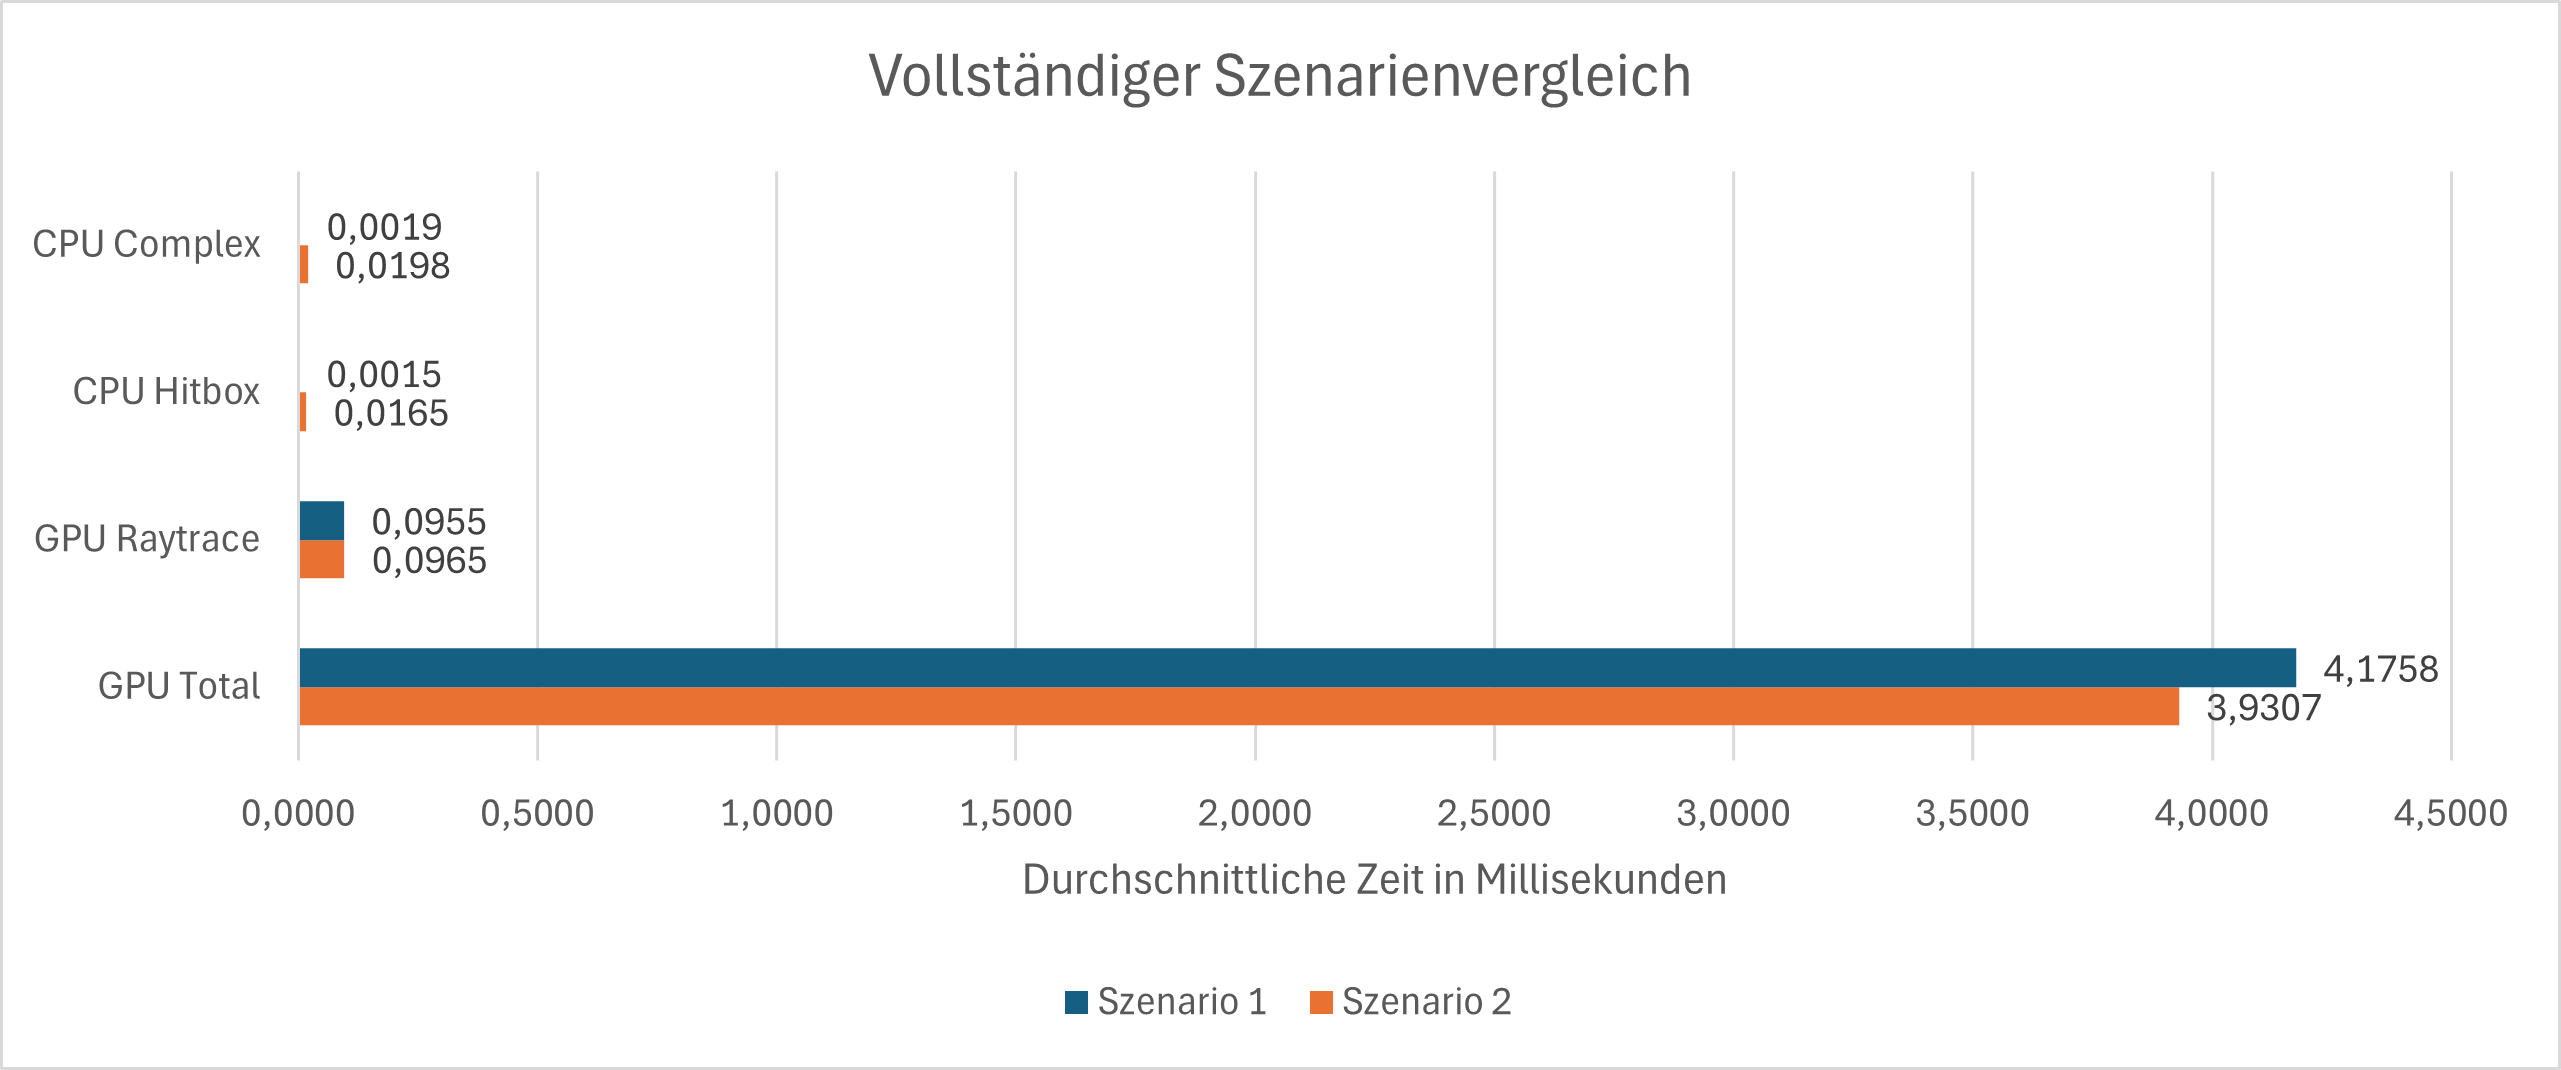
\includegraphics[width=0.7\linewidth]{Figures/full_comp_average}
		\caption[Vollständiger Szenarienvergleich Durchschnittszeit]{Die durchschnittliche Zeit aller Implementationen in beiden Szenarien}
		\label{fig:fullcompaverage}
	\end{figure}
	
	\pagebreak
	
	Die Zeit zum Erstellen der BLAS schwankt insgesamt zwischen beiden Szenarien stark. Wenngleich der Median beider wenig voneinander abweicht. Selbiges gilt für die TLAS. Extrema sind hier weniger stark voneinander abweichend. Siehe dazu Abbildung \ref{fig:blastlascomp}.
	
	\begin{figure}[h!]
		\centering
		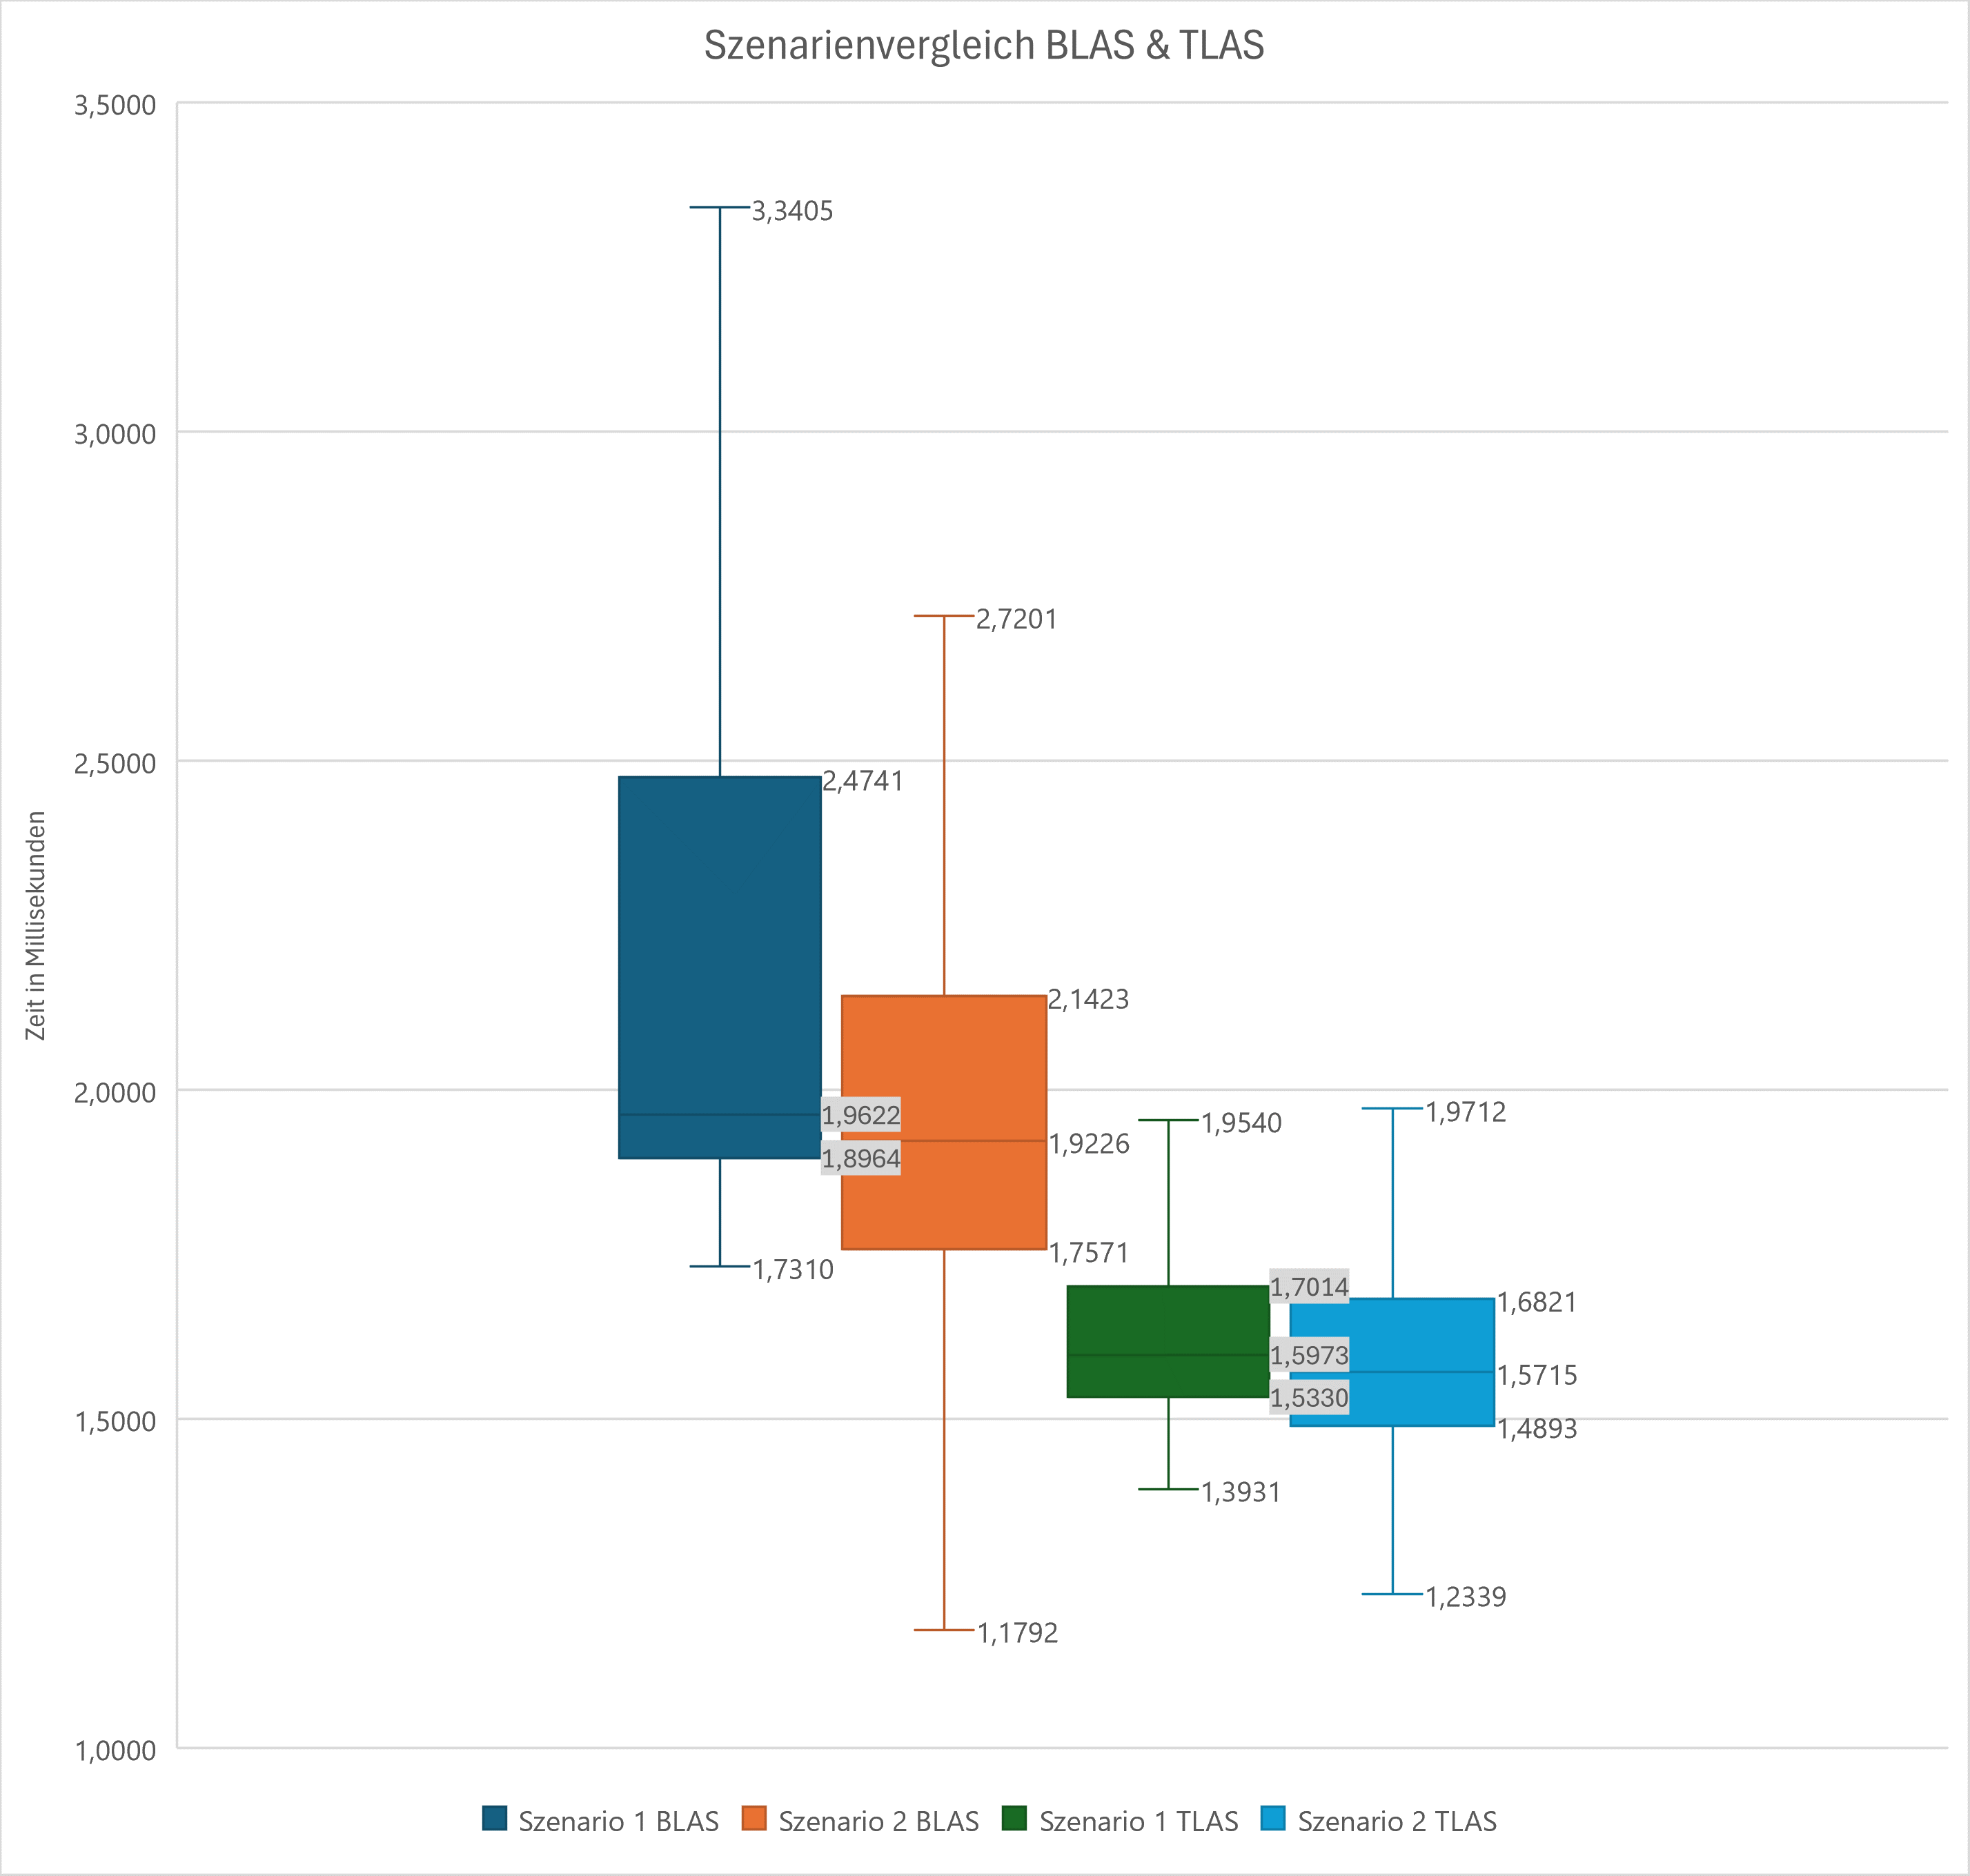
\includegraphics[width=0.7\linewidth]{Figures/rt_blas_tlas_comp.png}
		\caption[Szenarienvergleich BLAS \& TLAS Erstellung]{Boxplots der BLAS \& TLAS Generierung beider Szenarien}
		\label{fig:blastlascomp}
	\end{figure}
	
	\pagebreak
	
	Das Aufnehmen der Command Buffer in Abbildung \ref{fig:cmdbufcomp} ist annähernd identisch mit minimal abweichenden Extrema und bewegt sich im Rahmen zwischen \textit{19} bis \textit{40} Mikrosekunden.

	\begin{figure}[h!]
		\centering
		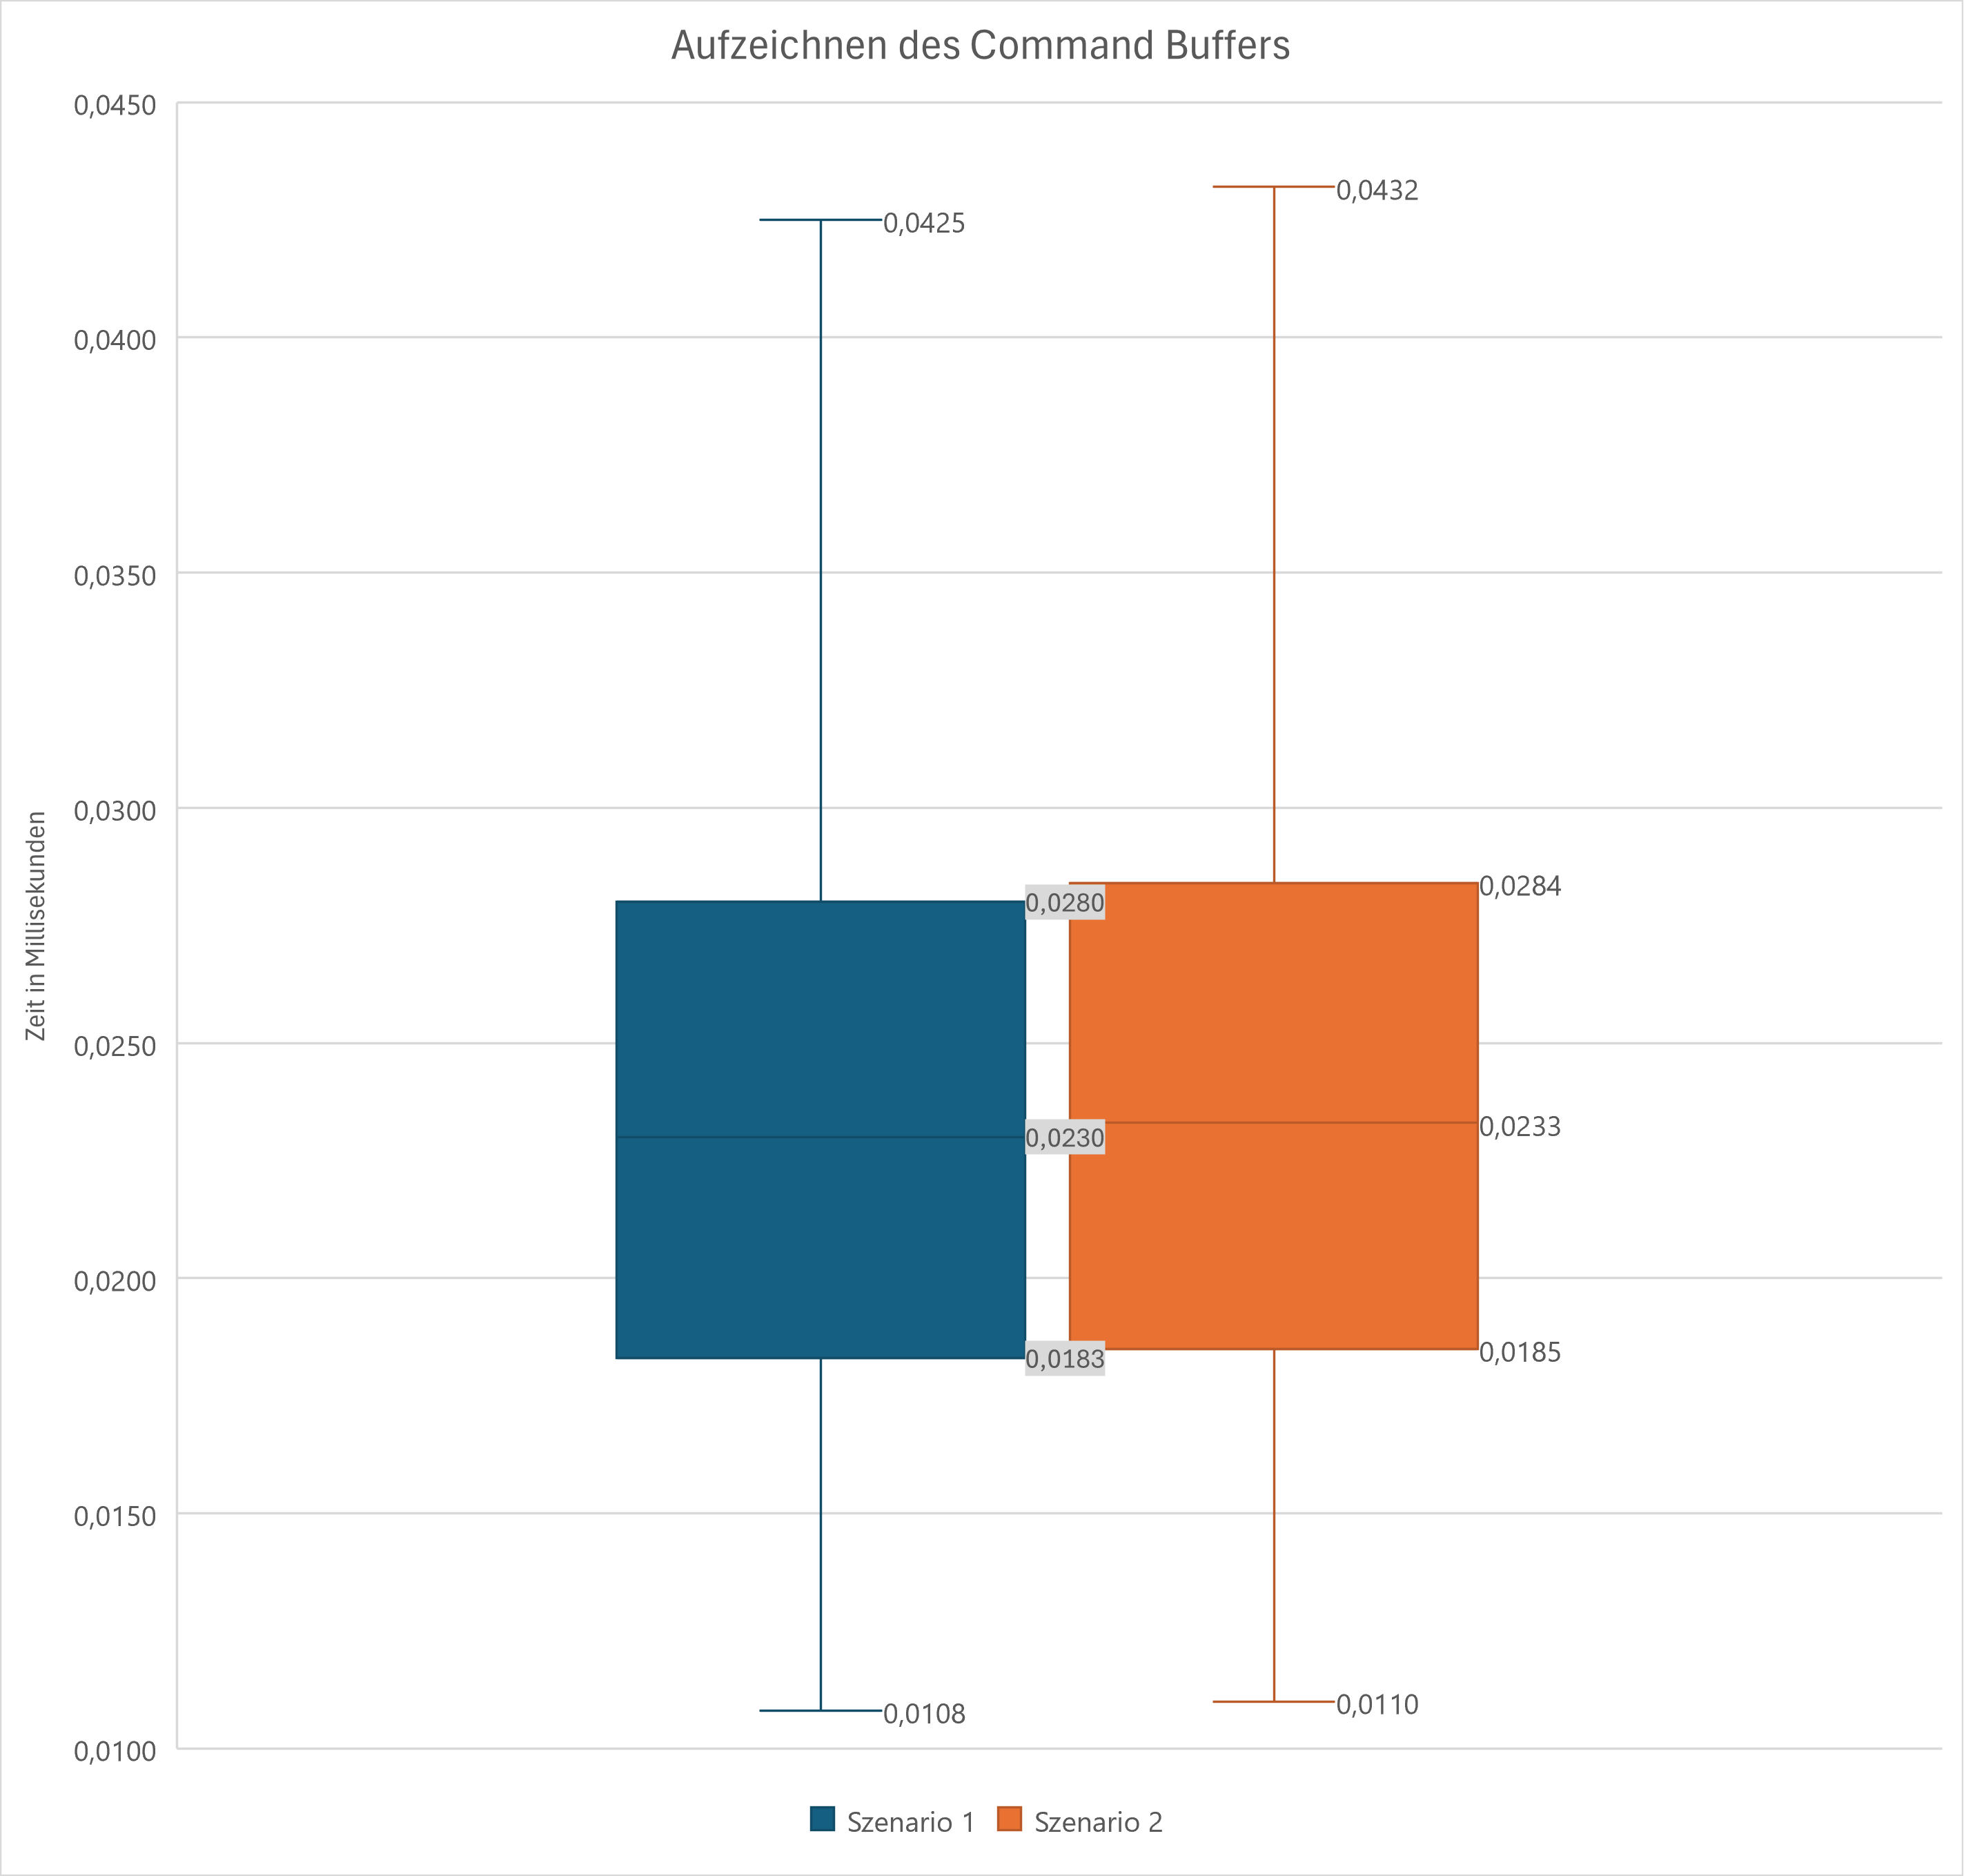
\includegraphics[width=0.7\linewidth]{Figures/rt_cmdbuf_comp.png}
		\caption[Szenarienvergleich Command Buffer Aufzeichnung]{Boxplots des Aufzeichnen der Command Buffer beider Szenarien}
		\label{fig:cmdbufcomp}
	\end{figure}
	
	\pagebreak
	
	Abbildung \ref{fig:resultscomp} zeigt eine \textit{10}-fache Steigerung der benötigten Zeit zum Transfer der Ergebnisse von der GPU zur CPU in Szenario Zwei gegenüber Szenario Eins.
	
	\begin{figure}[h!]
		\centering
		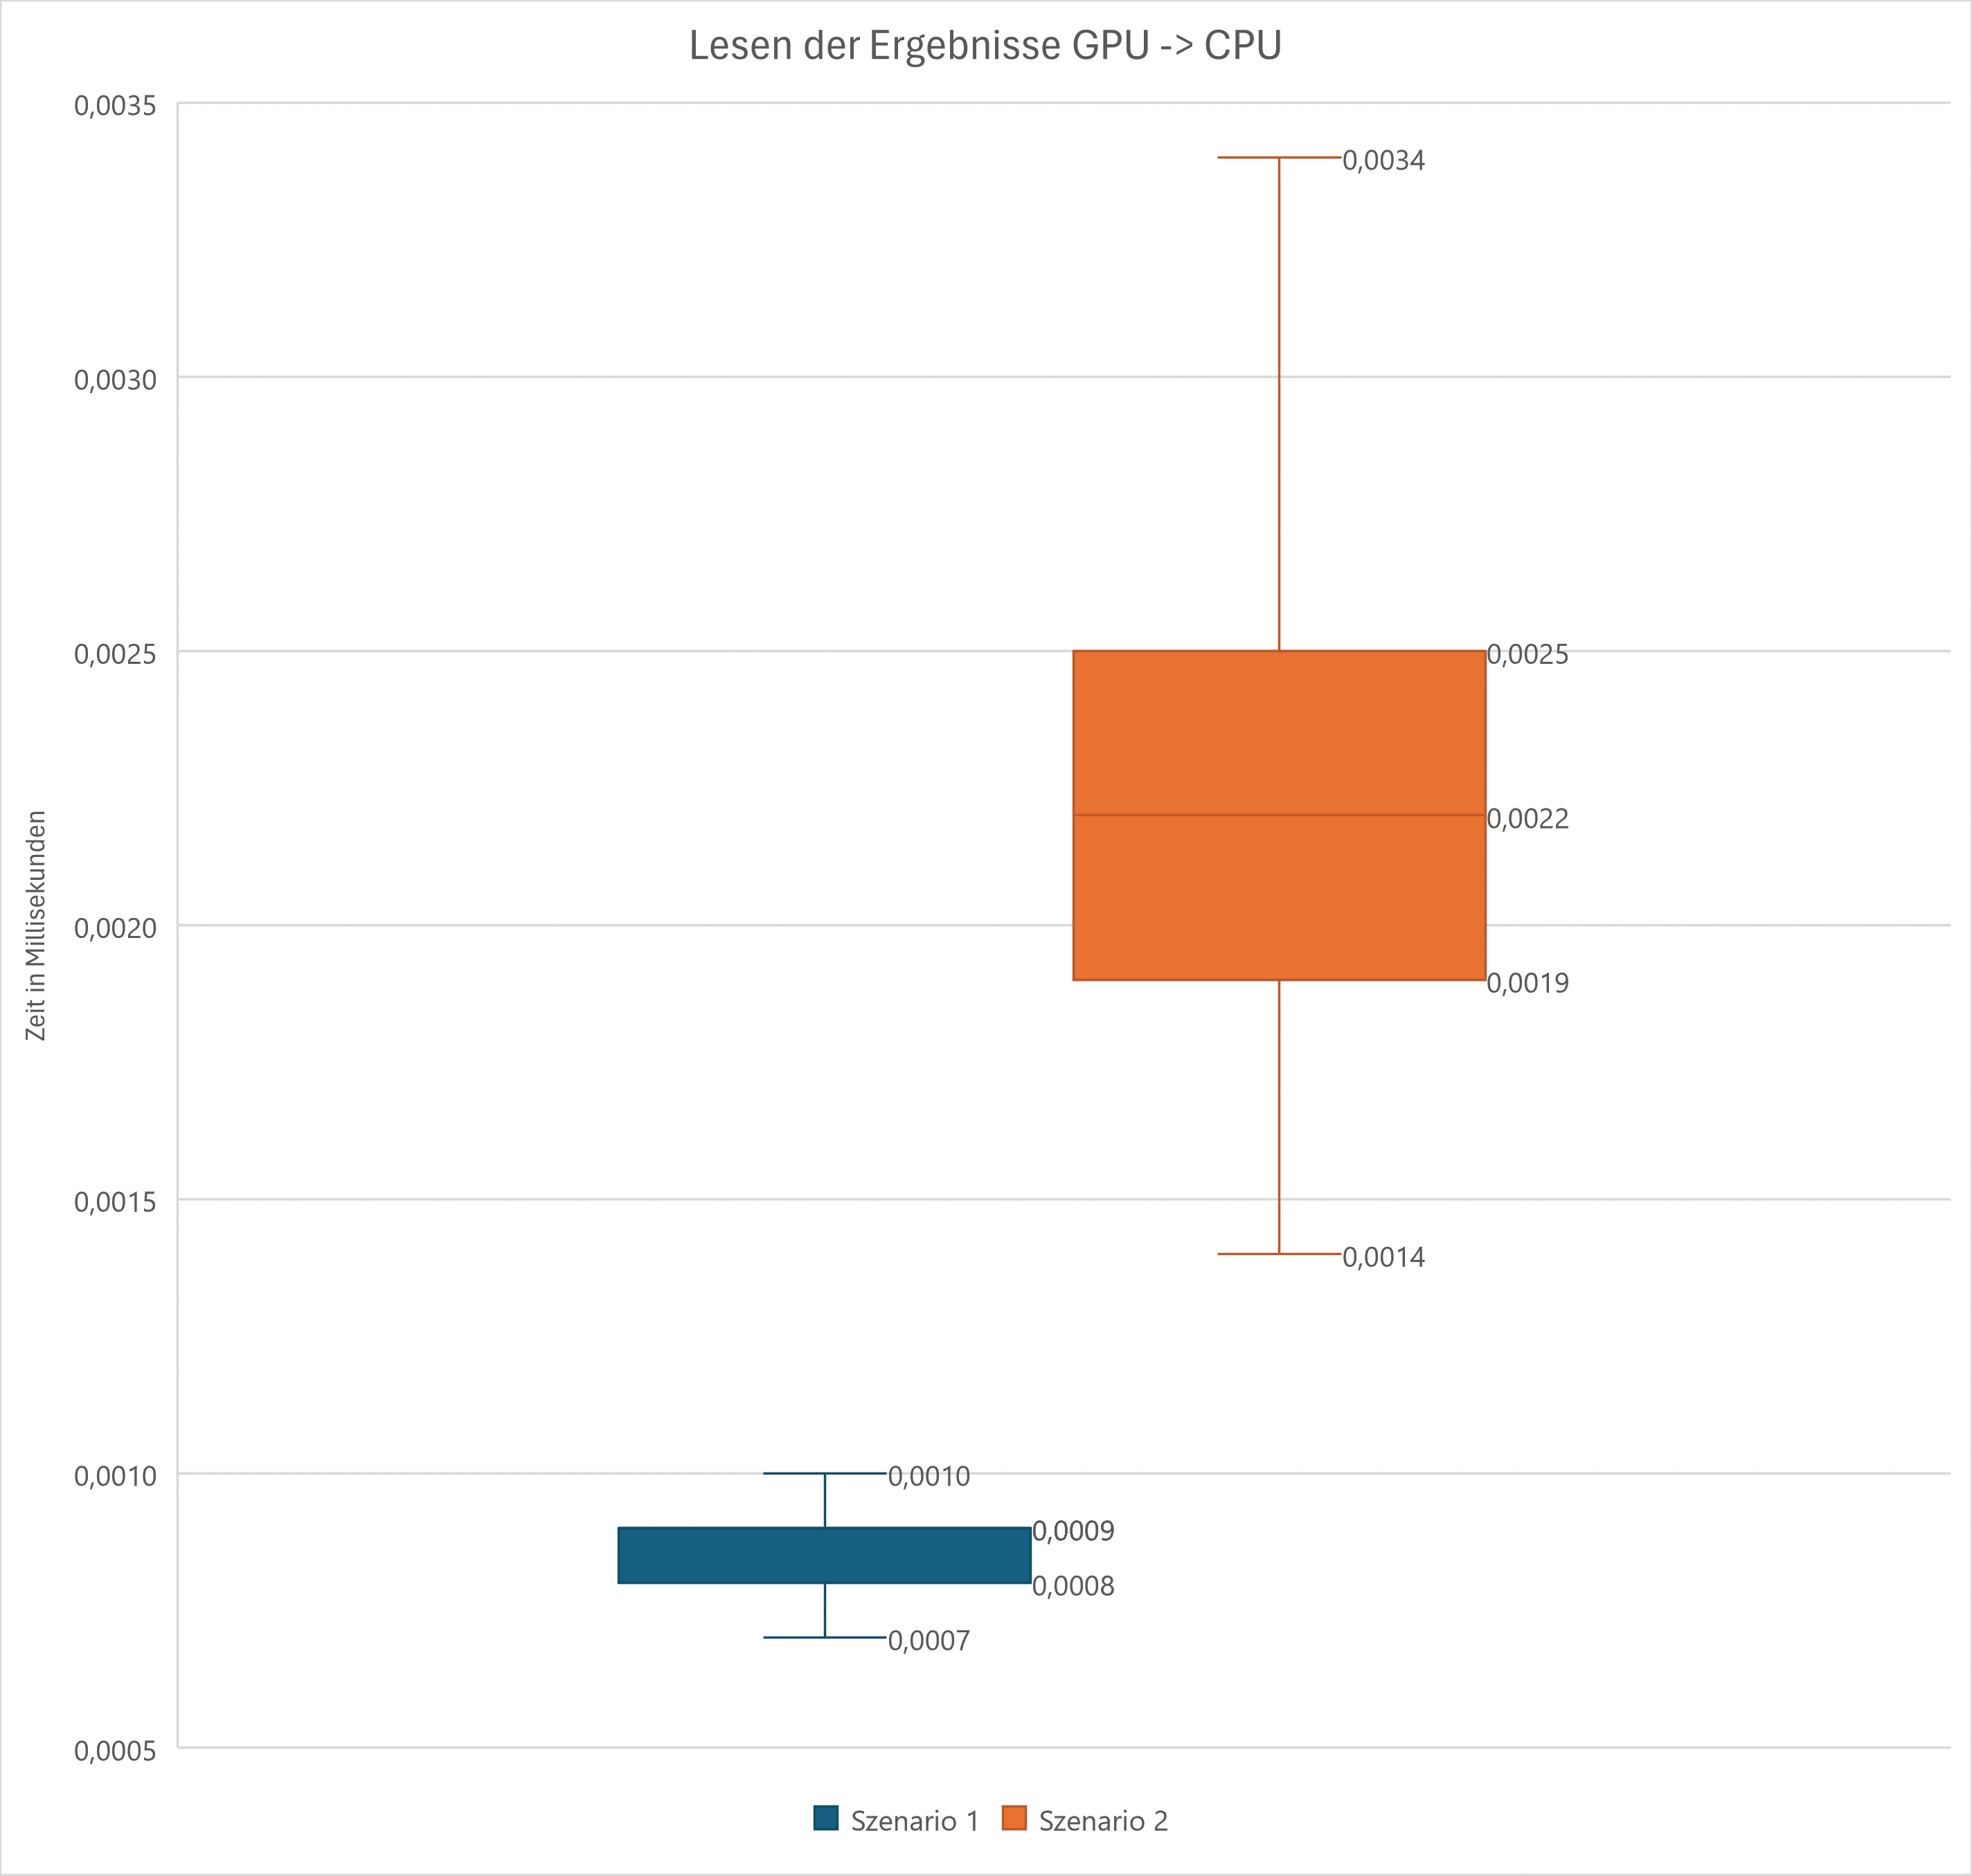
\includegraphics[width=0.7\linewidth]{Figures/rt_resultread_comp.png}
		\caption[Szenarienvergleich Transfer der Ergebnisse GPU->CPU]{Boxplots der benötigten Zeit zum Transfer der Ergebnisse von GPU->CPU beider Szenarien}
		\label{fig:resultscomp}
	\end{figure}
	
	\pagebreak
	
	
	Die Aufräumzeit der BLAS \& TLAS vom vorigen traceRays Durchlauf ist in beiden Szenarien annähernd gleich mit \textit{0,2} Millisekunden, wie Abbildung \ref{fig:cleanupcomp} darstellt.
	
	\begin{figure}[h!]
		\centering
		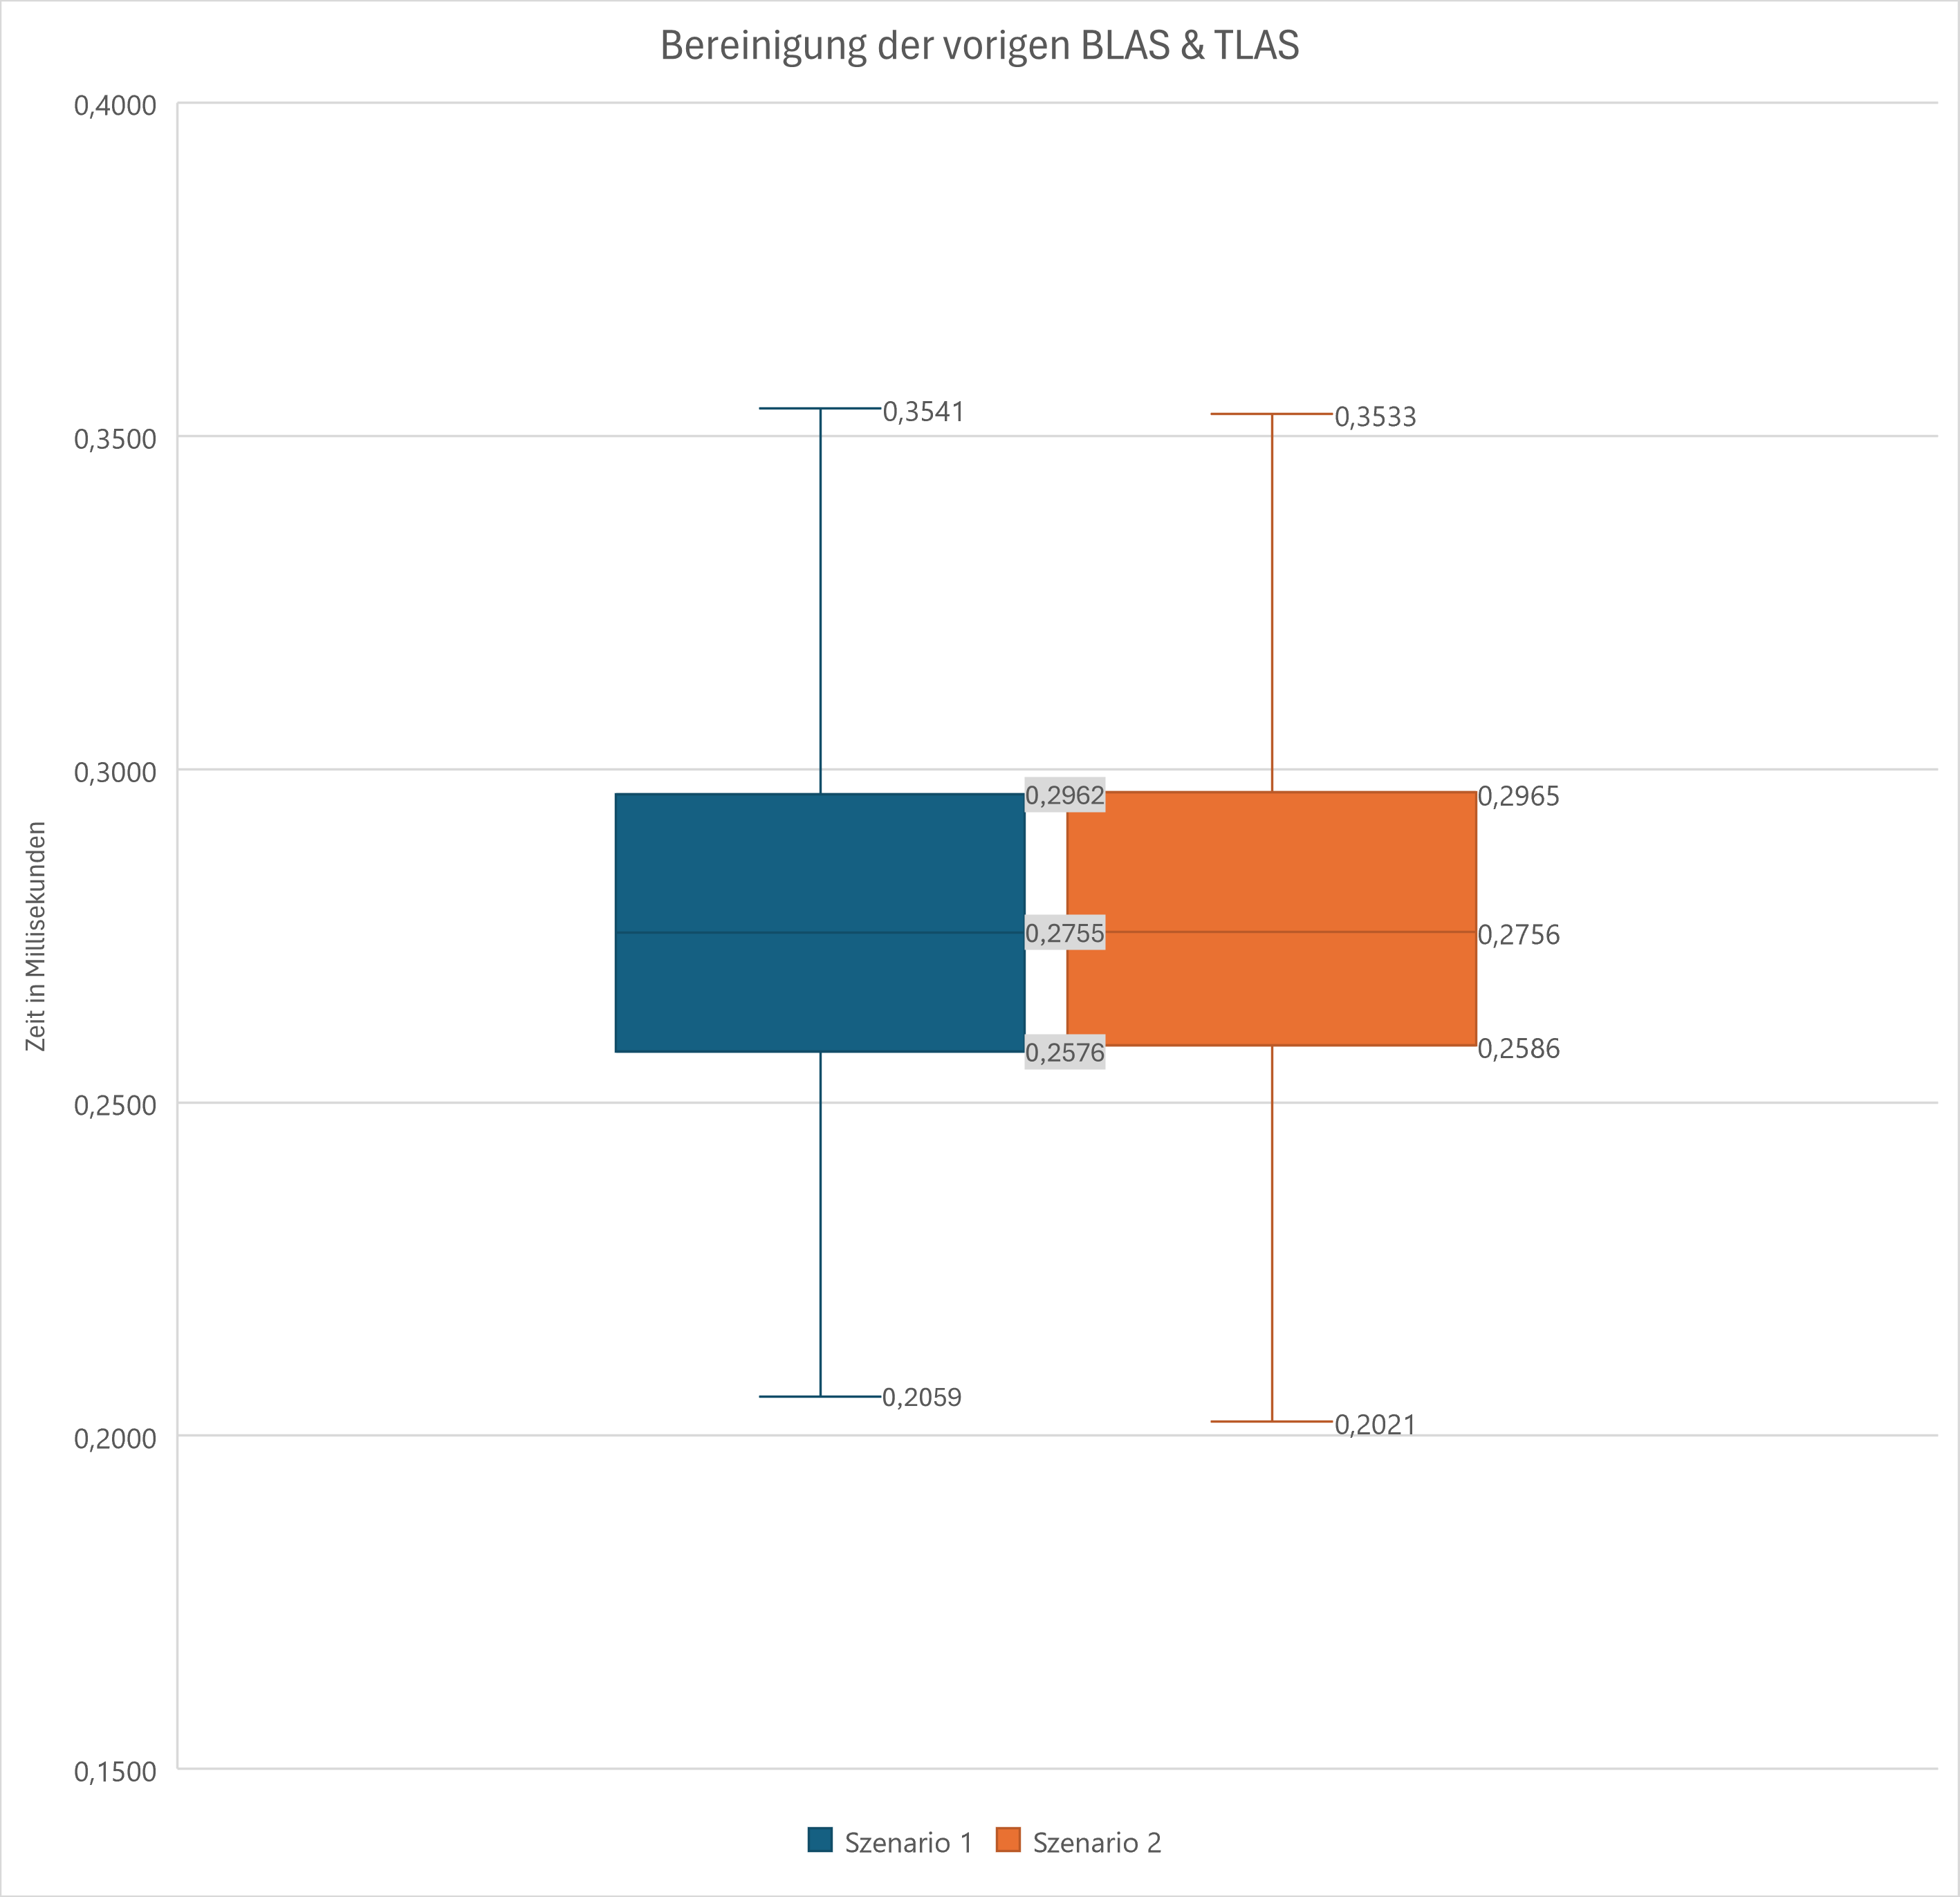
\includegraphics[width=0.7\linewidth]{Figures/rt_previous_cleanup.png}
		\caption[Szenarienvergleich Bereinigung voriger BLAS \& TLAS]{Boxplots der benötigten Zeit zum bereinigen der BLAS \& TLAS des vorigen Durchlaufs}
		\label{fig:cleanupcomp}
	\end{figure}
	
	Eine Ausnahme von den zuvor erwähnten Ausreißern sind die im Anhang in Abbildung \ref{fig:blastlascompoutliers} zu sehenden Ausreißer auf der Nulllinie der Y-Achse keine Lastspitzen durch andere Programme, sondern ergeben sich aus der Tatsache, dass beim allerersten Programmdurchlauf keine vorigen BLAS \& TLAS aufgeräumt werden müssen.
	
	\pagebreak
	
	Abschließend schlüsselt Abbildung \ref{fig:ue5comp} die Boxplots der Szenarien in UE5 zusammen mit den \textit{Hitbox} und \textit{Complex} Durchläufen detailliert auf.
	Szenario Eins ist in beiden Varianten sowohl bei Median als auch Extrema in \textit{einstelligen} Mikrosekundenbereich. Szenario Zwei hingegen zeigt eine größere Streuung. Dennoch bewegen sich beide Varianten im niedrigen \textit{zweistelligen} Mikrosekundenbereich.
	
	\begin{figure}[h!]
		\centering
		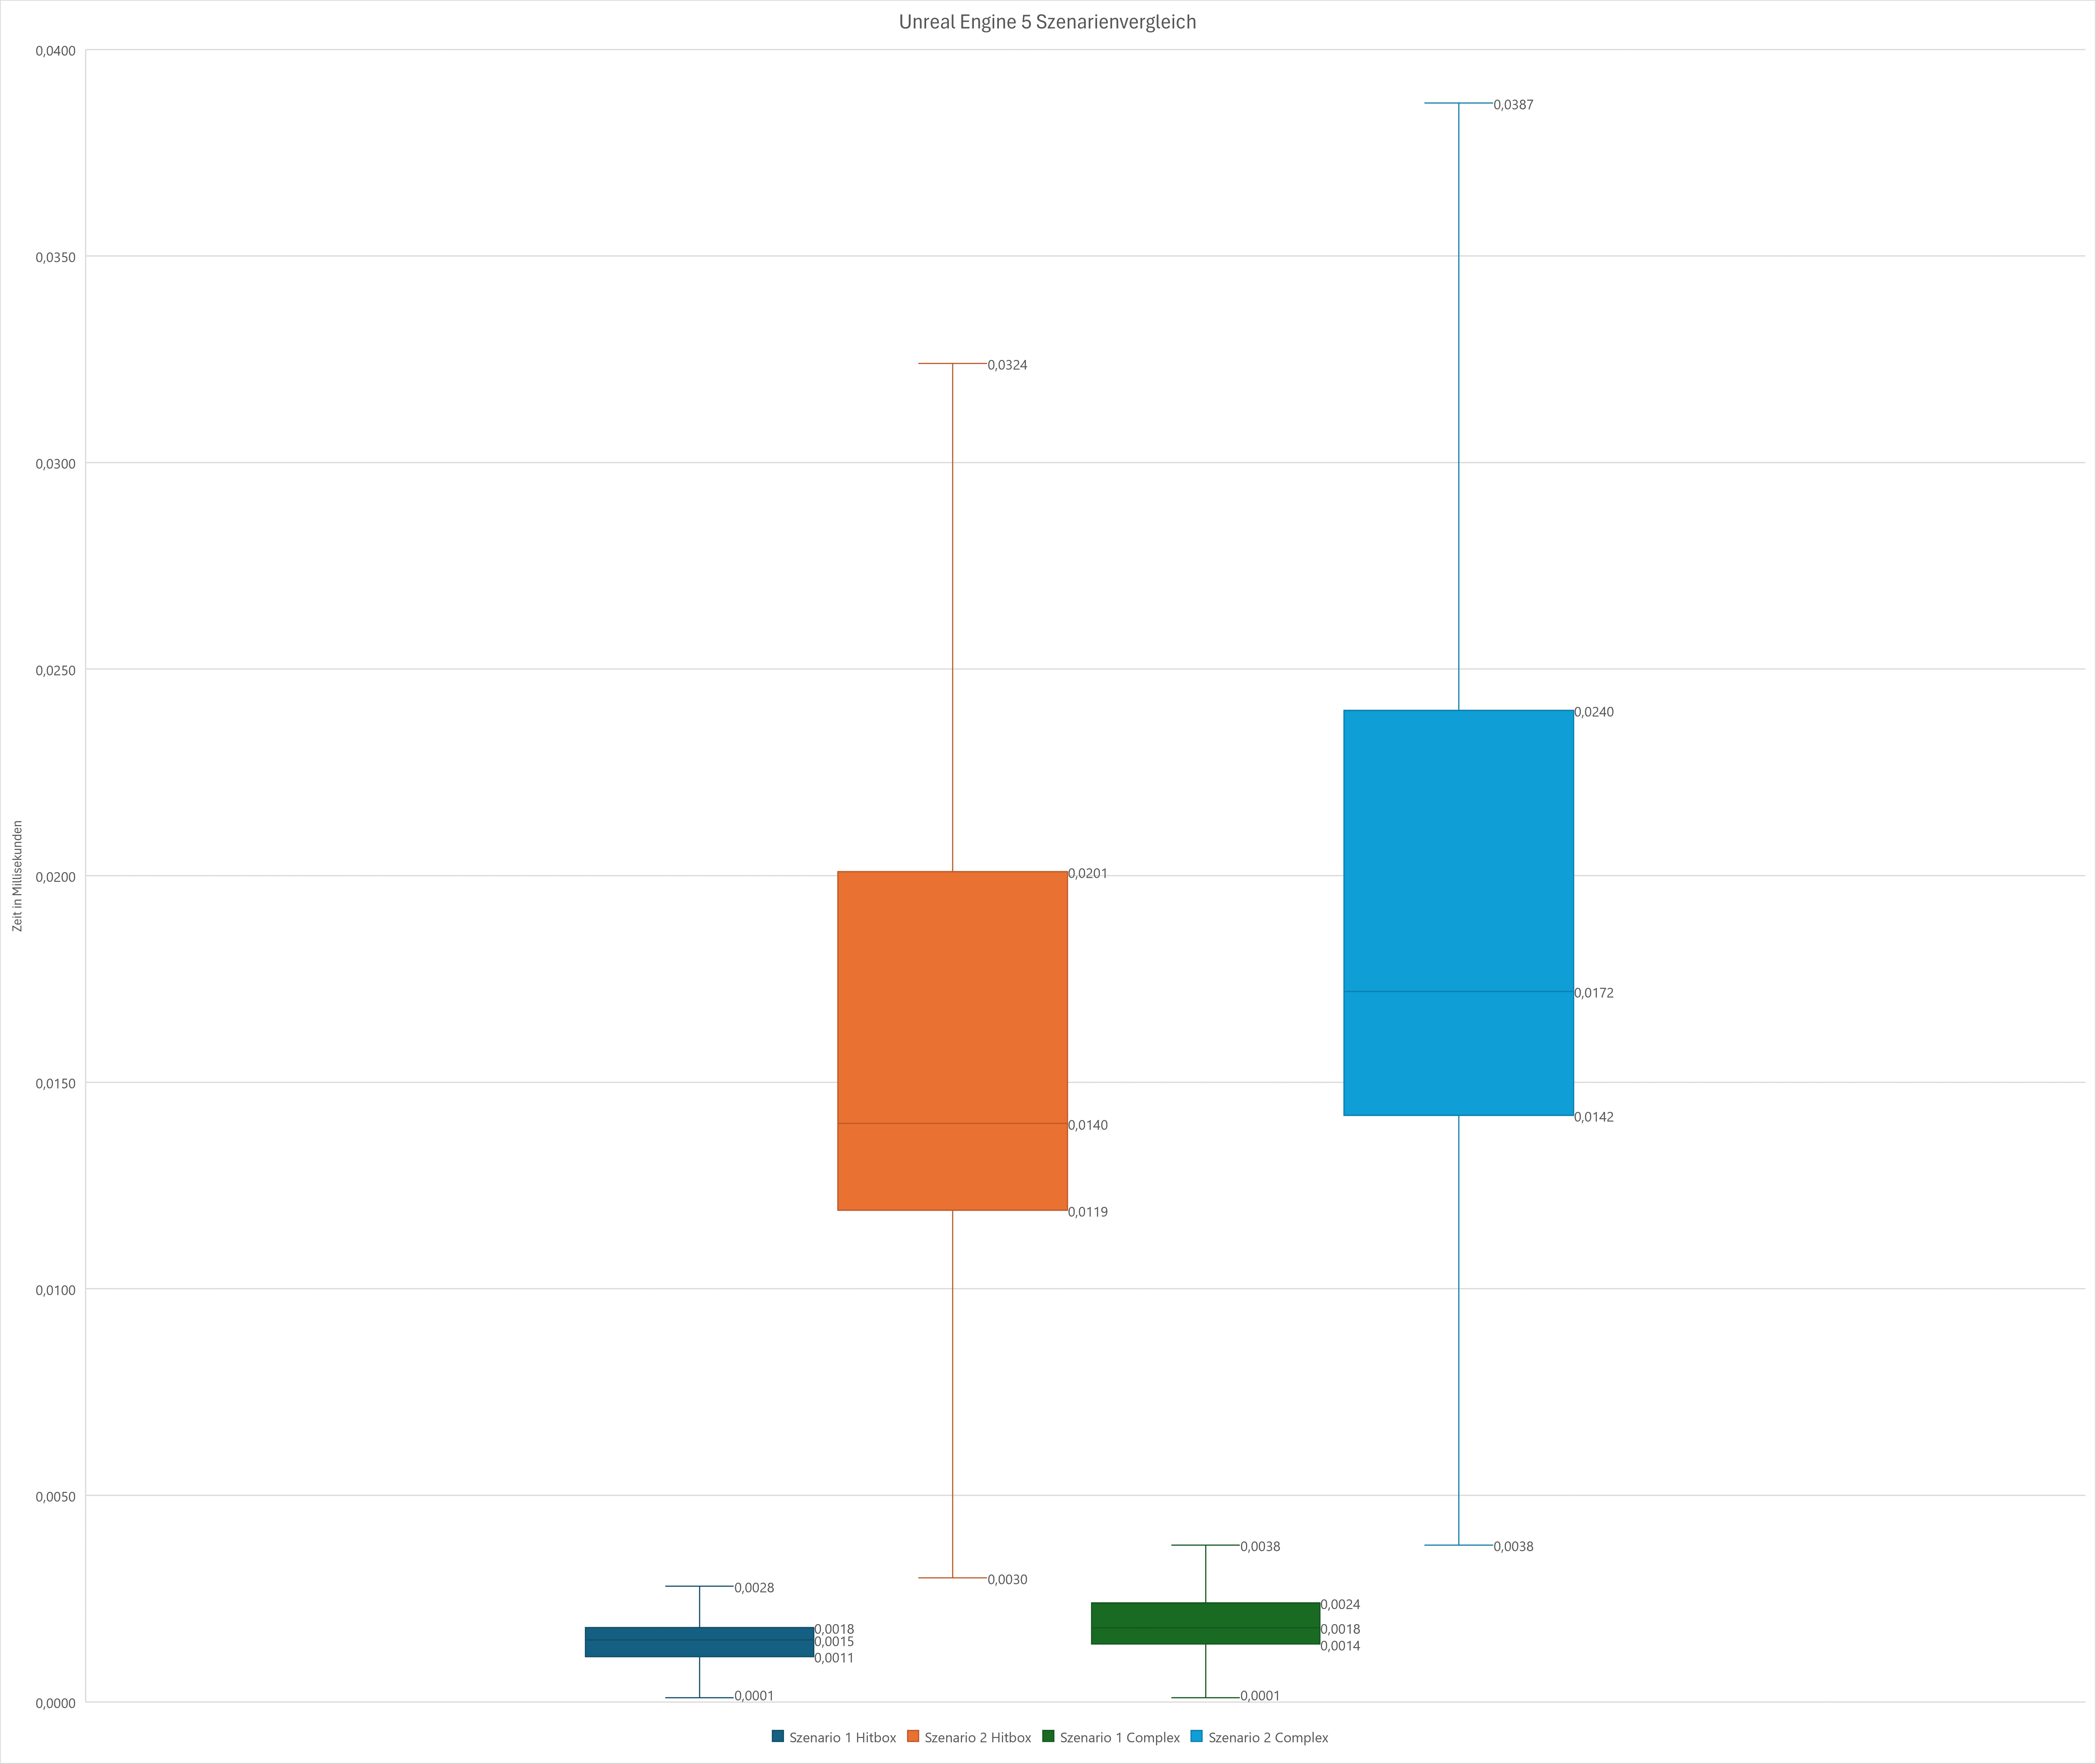
\includegraphics[width=1\linewidth]{Figures/rt_ue5_full_comp.png}
		\caption[Detaillierter Szenarienvergleich in UE5]{Boxplots der Szenarien und Varianten in UE5}
		\label{fig:ue5comp}
	\end{figure}
	
	
	\pagebreak
	\section{Zusammenfassung und Ausblick}
	Wie die Evaluation eindeutig zeigt, ist das Hardware-basierte GPU-Raytracing mit Vulkan Ray Queries signifikant langsamer. Betrachtet man zudem die Zeit, welche benötigt wird um die BLAS \& TLAS zu erzeugen, wird klar, dass diese Technik mehrere Millisekunden an Zeit kostet. In Videospielen ist dies zu lang. Die Ursachen können hierbei vielfältig sein. Einerseits könnte es an fehlenden oder inkorrekt gesetzten Vulkan-Flags liegen, andererseits könnte die PCI-E Schnittstelle nicht schnell genug sein. Auch überrascht es wie schnell die \textit{UE5 Complex} Variante ist. Allerdings gilt es hierbei zu beachten dass lediglich ein einziges 3D-Modell getestet wurde. Bei dem Schrotflinten-Szenario wurde die Hochparallelisierung der Grafikkarte deutlich. Die reinen GPU-Raytracing Zeiten unterscheiden sich in beiden Szenarien minimal voneinander während die UE5 Testdaten eine Steigerung des Berechnungsaufwandes zeigen. In dieser Arbeit wurden nur statische 3D-Modelle betrachtet. Die Instanzen unterscheiden sich hierbei nur in Position, Rotation und Skalierung. in Videospielen kommen jedoch auch sehr viele animierte 3D-Modelle vor. Die Geometrie verformt sich. Hier könnte der GPU-Ansatz aufgrund der Parallelisierung einen Vorteil haben. Weiterführende Forschungen zu dieser Arbeit könnten die Nutzung von Machine Learning zur weiteren Performance-Steigerung der Treffererkennung analog dem existierenden DLSS Ray Reconstruction sowie die Integration von Machine Learning in existierende CPU-basierte Physik-Engines sein.
	
	 Abschließend lassen der aktuelle Forschungsstand sowie die technologische Weiterentwicklung der RT-Kerne und des Machine Learnings hoffen, dass Treffererkennung auf Grafikkarten die aktuell eingesetzten Hitboxen in näherer Zukunft ersetzt.


	\pagebreak
	\section{Literaturverzeichnis}
	%---------------------------------
	% LITERATUR
	%---------------------------------
	%\bibliographystyle{IEEEtran}
	%\bibliography{IEEEabrv,literatur}
	%\bibliographystyle{plain}
	%\bibliography{literatur}
	
	
	% Gesamte Literaturliste
	%\printbibliography	
	% Literaturliste getrennt in Papier- und Online-Quellen:
	\printbibliography[nottype=online, heading=subbibliography, title={Gedruckte Quellen}]
	\printbibliography[type=online, heading=subbibliography, title={Online-Quellen}]
	
	
	\pagebreak
	\section{Listingverzeichnis}
	\makeatletter
	\renewcommand*\l@lstlisting{\@dottedtocline{1}{0em}{2em}} % Entfernt den Einzug für die Listings
	\renewcommand*\lstlistoflistings{
		\@starttoc{lol}
	}
	\makeatother
	\lstlistoflistings
	

	\pagebreak
	\section{Abbildungsverzeichnis}
	\makeatletter
	\renewcommand\listoffigures{
		\@starttoc{lof}
	}
	\makeatother	
	\listoffigures
	
	\pagebreak
	\section{Glossar}
	\renewcommand{\glossarypreamble}{}
	\renewcommand{\glossarysection}[2][]{} % Falls keine Sektion erstellt werden soll
	\printglossary[title=]
	
	\pagebreak
	\section{Akronyme}
	\printglossary[type=\acronymtype, title=]
	
	\pagebreak
	\section{Anhangsverzeichnis}
	
	\appendix
	\vspace{-3.12em} % Forcefully remove the whitespace of the empty title so it matches the distance like in other tocs
	\listofappendices % Anhangsverzeichnis#
	
	\pagebreak
	
	\appendixitem{BVH-Algorithmus Visualisierung}
	\begin{figure}[h]
		\centering
		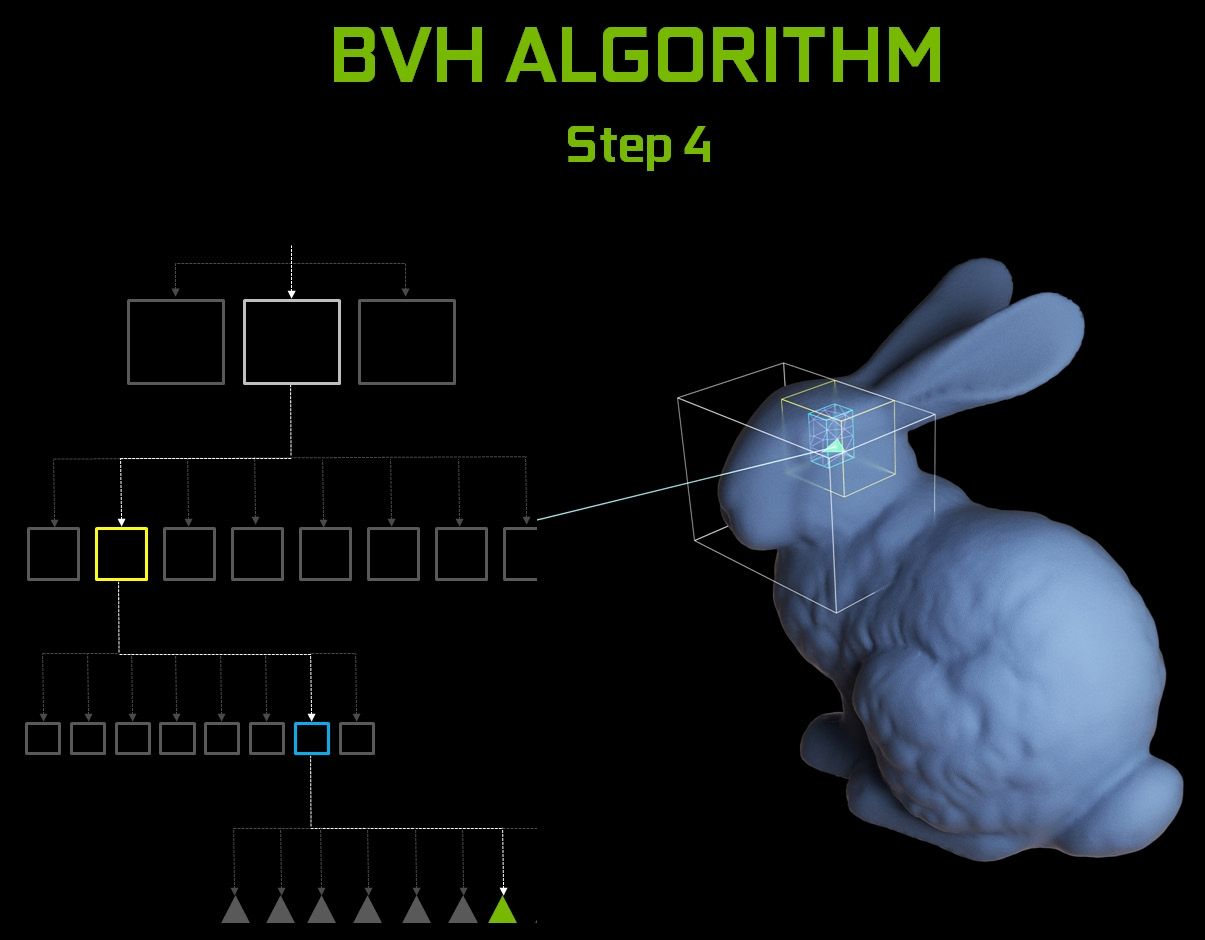
\includegraphics[width=0.7\linewidth]{Figures/rt_cores_bvh_explained}
		\caption[Darstellung des Bounding Volume Hierarchy-Algorithmus auf RT-Kernen]{Darstellung des Bounding Volume Hierarchy-Algorithmus auf RT-Kernen\cite{Corporation2018}}
		\label{fig:rtcoresbvhexplained}
	\end{figure}
	
	\appendixitem{Compute-Pipeline Initialisierung}
	\begin{lstlisting}[caption={Erstellen der Compute-Pipeline in VulkanRenderer.cpp},label={lst:listing-vulkan-computepipelinecpp}]
void VulkanRenderer::createComputePipeline()
	{
		...
		const auto computeShaderAsset = assetManager->getAsset<Assets::ShaderAsset>("Assets/Shaders/compute.comp.spv");
		...
		auto computeShaderModule = createShaderModule(computeShaderAsset->getShader());
		vk::PipelineShaderStageCreateInfo computeShaderStageInfo = {};
		computeShaderStageInfo.stage = vk::ShaderStageFlagBits::eCompute;
		computeShaderStageInfo.module = *computeShaderModule;
		computeShaderStageInfo.pName = "main";
		
		vk::PipelineLayoutCreateInfo pipelineLayoutInfo = {};
		pipelineLayoutInfo.setLayoutCount = 1;
		pipelineLayoutInfo.pSetLayouts = &computeDescriptorSetLayout;
		...
		computePipelineLayout = logicalDevice->createPipelineLayout(pipelineLayoutInfo);
		...	
		vk::ComputePipelineCreateInfo computePipelineCreateInfo = {};
		computePipelineCreateInfo.stage = computeShaderStageInfo;
		computePipelineCreateInfo.layout = computePipelineLayout;
		
		const auto computePipelineResult = logicalDevice->createComputePipeline(nullptr, computePipelineCreateInfo);
		...
		computePipeline = computePipelineResult.value;
		...
}	\end{lstlisting}

	\appendixitem{ComputeInputBufferObject-Klasse}
	\begin{lstlisting}[caption={\textit{ComputeInputBufferObject}-Klasse in ComputeInputBufferObject.hpp},label=lst:listing-vulkan-computeinputbuffer]
struct ComputeInputBufferObject
{
	alignas(16) glm::vec3 origin;
	alignas(16) glm::vec3 direction;
	alignas(4) float tMin;
	alignas(4) float tMax;
	alignas(4) uint32_t rayId;
};	\end{lstlisting}

	\appendixitem{ComputeOutputBufferObject-Klasse}
	\begin{lstlisting}[caption={\textit{ComputeOutputBufferObject}-Klasse in ComputeOutputBufferObject.hpp},label=lst:listing-vulkan-computeoutputbuffer]
struct ComputeOutputBufferObject
{
	alignas(8) uint32_t isHit;
	alignas(8) uint32_t rayId;
};	\end{lstlisting}


	\appendixitem{Descriptor Pool Erzeugung}
	\begin{lstlisting}[caption={Erstellen des Descriptor Pools in VulkanRenderer.cpp},label={lst:listing-vulkan-computedescriptorpoolcpp}]
void VulkanRenderer::createComputeDescriptorPool()
{
	constexpr vk::DescriptorPoolSize storageBufferpoolSize{vk::DescriptorType::eStorageBuffer, 1};
	constexpr vk::DescriptorPoolSize accelerationStructurePoolSize{
		vk::DescriptorType::eAccelerationStructureKHR, 1
	};
	constexpr std::array poolSizes = {accelerationStructurePoolSize, storageBufferpoolSize};
	const vk::DescriptorPoolCreateInfo poolInfo{
		{}, 1, static_cast<uint32_t>(poolSizes.size()), poolSizes.data()
	};
	...
	computeDescriptorPool = logicalDevice->createDescriptorPool(poolInfo);
	...
}	\end{lstlisting}

	\appendixitem{Descriptor Set Erzeugung}
	\begin{lstlisting}[caption={Erstellen des Descriptor Sets in VulkanRenderer.cpp},label={lst:listing-vulkan-computedescriptorsetcpp}]
void VulkanRenderer::createComputeDescriptorSet()
{
	vk::DescriptorSetAllocateInfo allocInfo = {};
	allocInfo.descriptorPool = computeDescriptorPool;
	allocInfo.descriptorSetCount = 1;
	allocInfo.pSetLayouts = &computeDescriptorSetLayout;
	...
	computeDescriptorSet = logicalDevice->allocateDescriptorSets(allocInfo)[0];
	...
	const vk::WriteDescriptorSetAccelerationStructureKHR tlasDescriptorWrite{
		1, &topLevelAccelerationStructure.accelerationStructureKHR
	};
	vk::WriteDescriptorSet accelerationStructureDescriptorWrite{};
	accelerationStructureDescriptorWrite.dstSet = computeDescriptorSet;
	accelerationStructureDescriptorWrite.dstBinding = 0;
	accelerationStructureDescriptorWrite.dstArrayElement = 0;
	accelerationStructureDescriptorWrite.descriptorType = vk::DescriptorType::eAccelerationStructureKHR;
	accelerationStructureDescriptorWrite.descriptorCount = 1;
	accelerationStructureDescriptorWrite.pNext = &tlasDescriptorWrite;
	const vk::DescriptorBufferInfo inputBufferInfo{inputComputeBuffer, 0, sizeof(ComputeInputBufferObject)};
	vk::WriteDescriptorSet inputDescriptorWrite = {};
	inputDescriptorWrite.dstSet = computeDescriptorSet;
	inputDescriptorWrite.dstBinding = 1;
	inputDescriptorWrite.dstArrayElement = 0;
	inputDescriptorWrite.descriptorType = vk::DescriptorType::eStorageBuffer;
	inputDescriptorWrite.descriptorCount = 1;
	inputDescriptorWrite.pBufferInfo = &inputBufferInfo;
	const vk::DescriptorBufferInfo outputBufferInfo{outputComputeBuffer, 0, sizeof(ComputeOutputBufferObject)};
	vk::WriteDescriptorSet outputDescriptorWrite = {};
	outputDescriptorWrite.dstSet = computeDescriptorSet;
	outputDescriptorWrite.dstBinding = 2;
	outputDescriptorWrite.dstArrayElement = 0;
	outputDescriptorWrite.descriptorType = vk::DescriptorType::eStorageBuffer;
	outputDescriptorWrite.descriptorCount = 1;
	outputDescriptorWrite.pBufferInfo = &outputBufferInfo;
	const std::array descriptorWrites = {
		accelerationStructureDescriptorWrite, inputDescriptorWrite, outputDescriptorWrite
	};
	logicalDevice->updateDescriptorSets(descriptorWrites, nullptr);
}	\end{lstlisting}

	\appendixitem{Compute Command Pool Erstellung}
	\begin{lstlisting}[caption={Erstellen des Compute Command Pools in VulkanRenderer.cpp},label={lst:listing-vulkan-computecommandpoolcpp}]
void VulkanRenderer::createComputeCommandPool()
{
	const QueueFamilyIndices queueFamilyIndices = findQueueFamilies(physicalDevice);
	vk::CommandPoolCreateInfo poolInfo = {};
	poolInfo.flags = vk::CommandPoolCreateFlagBits::eTransient;
	poolInfo.queueFamilyIndex = queueFamilyIndices.computeFamily.value();
	...
	computeCommandPool = logicalDevice->createCommandPool(poolInfo);
	...
}	\end{lstlisting}

	\pagebreak
	\appendixitem{UE5 3D-Modell mit Hitboxen}
	\begin{figure}[h]
		\centering
		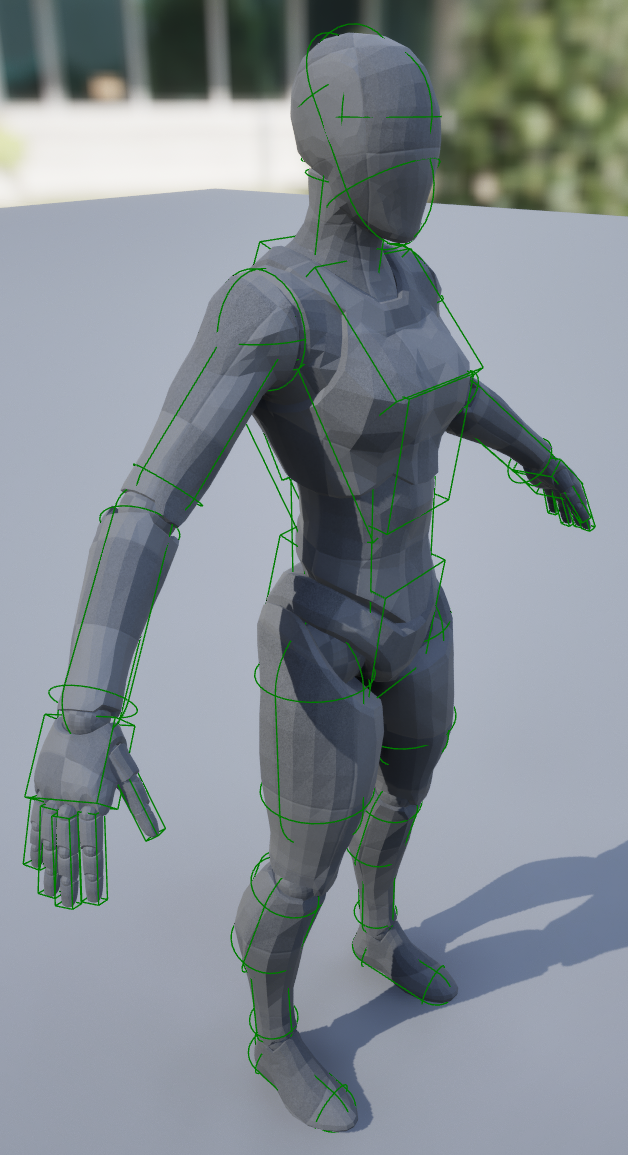
\includegraphics[width=0.5\linewidth]{Figures/hitboxes}
		\caption[UE5 3D-Modell mit Hitboxen]{Darstellung des verwendeten 3D-Modells mit Hitboxen}
		\label{fig:hitboxes}
	\end{figure}
	\pagebreak
	\appendixitem{Szenarienvergleich BLAS \& TLAS Erstellung mit Ausreißern}
	\begin{figure}[h!]
		\centering
		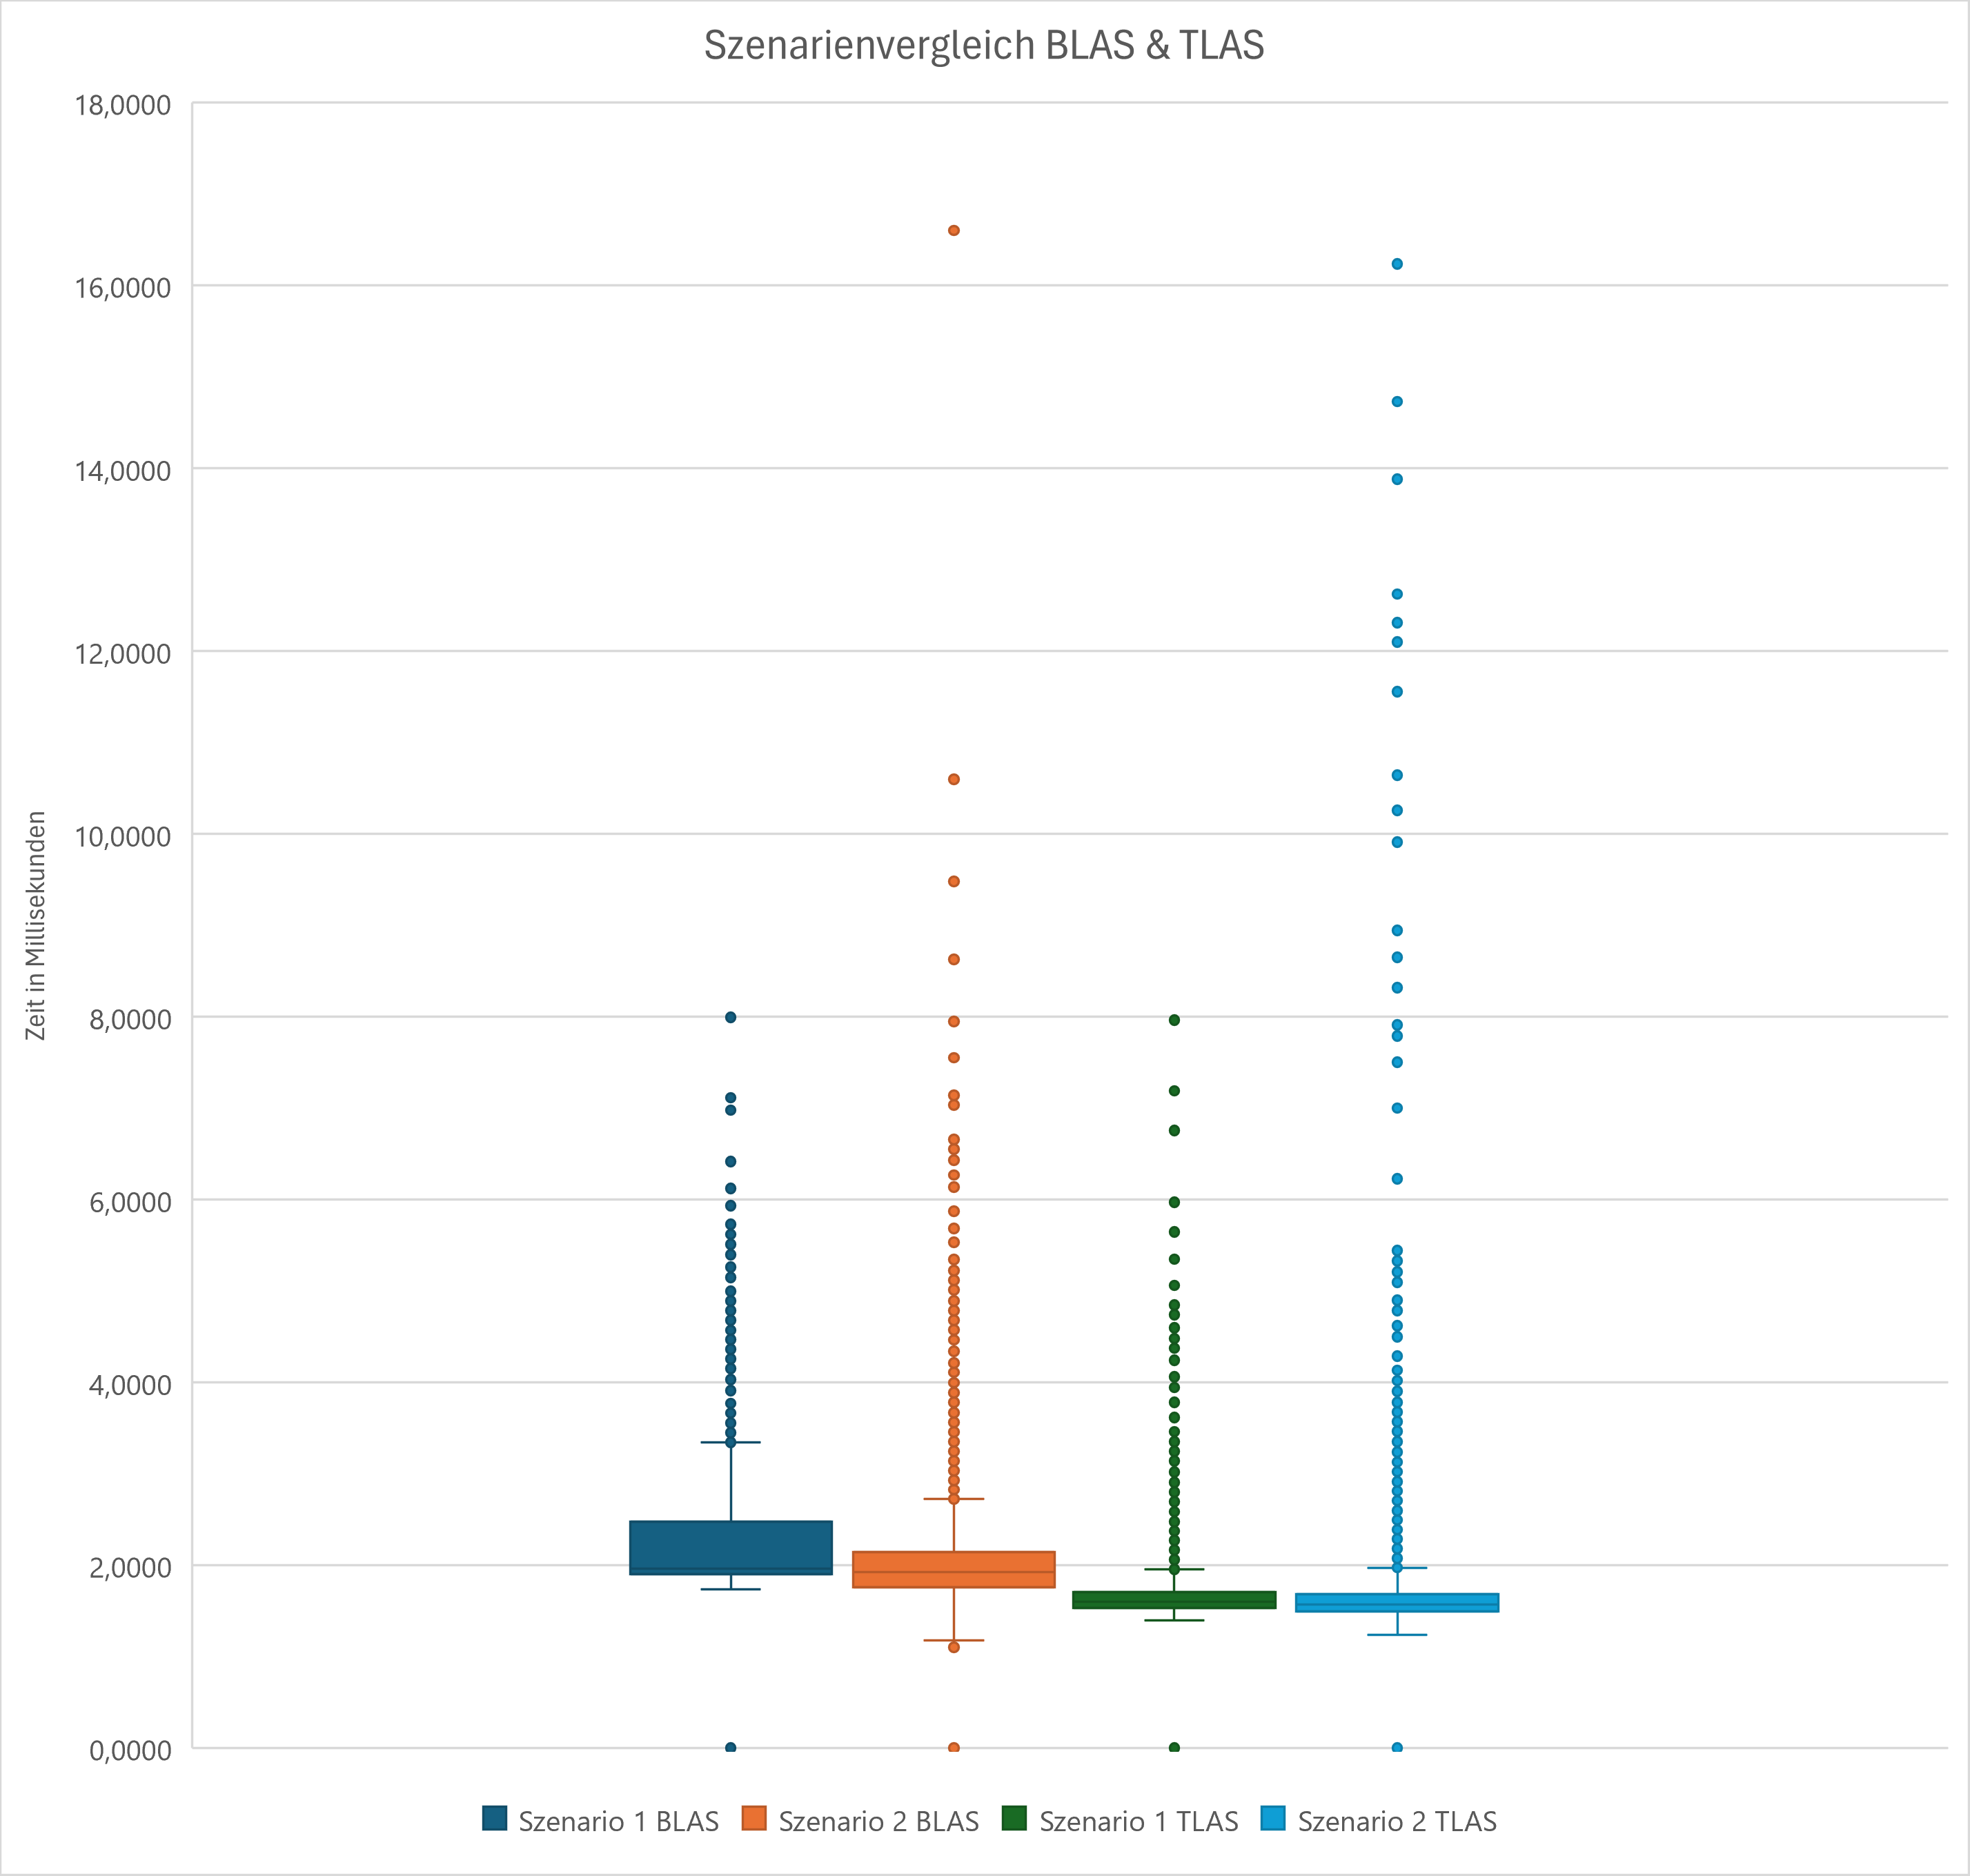
\includegraphics[width=0.7\linewidth]{Figures/rt_blas_tlas_comp_outliers.png}
		\caption[Szenarienvergleich BLAS \& TLAS Erstellung mit Ausreißern]{Boxplots der BLAS \& TLAS Generierung beider Szenarien mit Ausreißern}
		\label{fig:blastlascompoutliers}
	\end{figure}
	\pagebreak
	\appendixitem{Szenarienvergleich Command Buffer Aufzeichnung mit Ausreißern}
	\begin{figure}[h!]
		\centering
		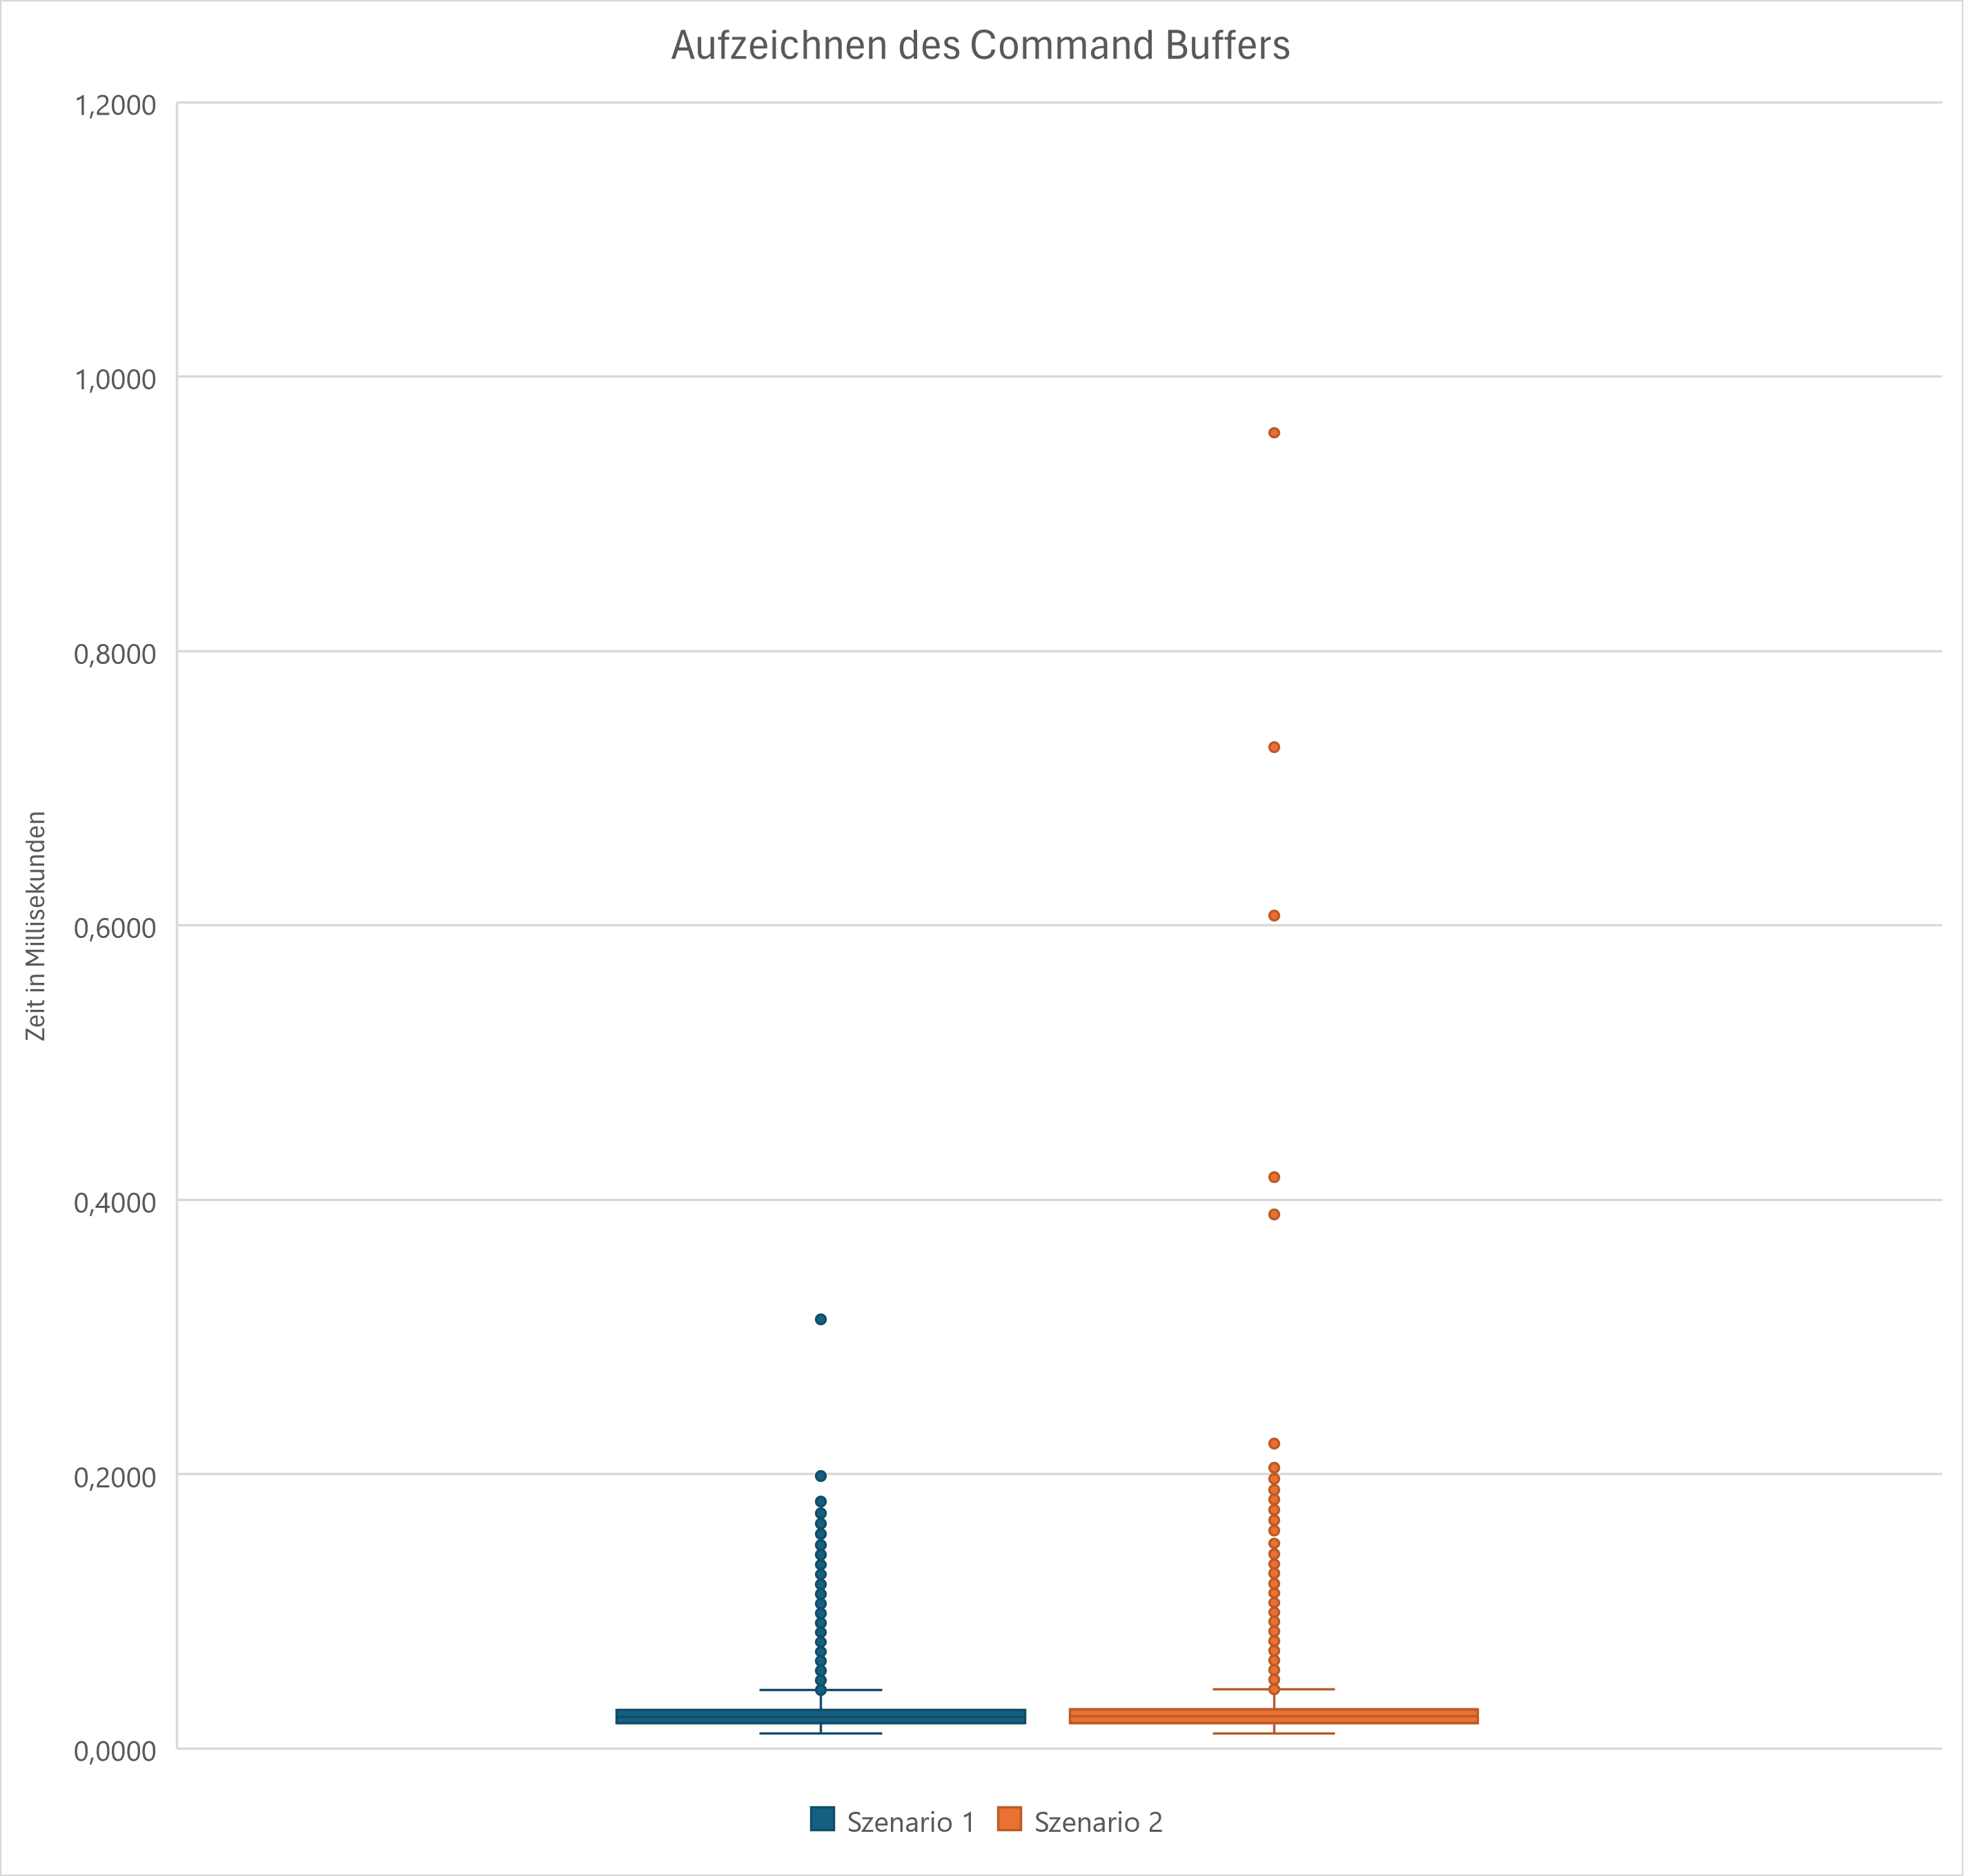
\includegraphics[width=0.7\linewidth]{Figures/rt_cmdbuf_comp_outliers.png}
		\caption[Szenarienvergleich Command Buffer Aufzeichnung mit Ausreißern]{Boxplots des Aufzeichnen der Command Buffer beider Szenarien mit Ausreißern}
		\label{fig:cmdbufcompoutliers}
	\end{figure}
	\pagebreak
	\appendixitem{Szenarienvergleich Transfer der Ergebnisse GPU->CPU mit Ausreißern}
	\begin{figure}[h!]
		\centering
		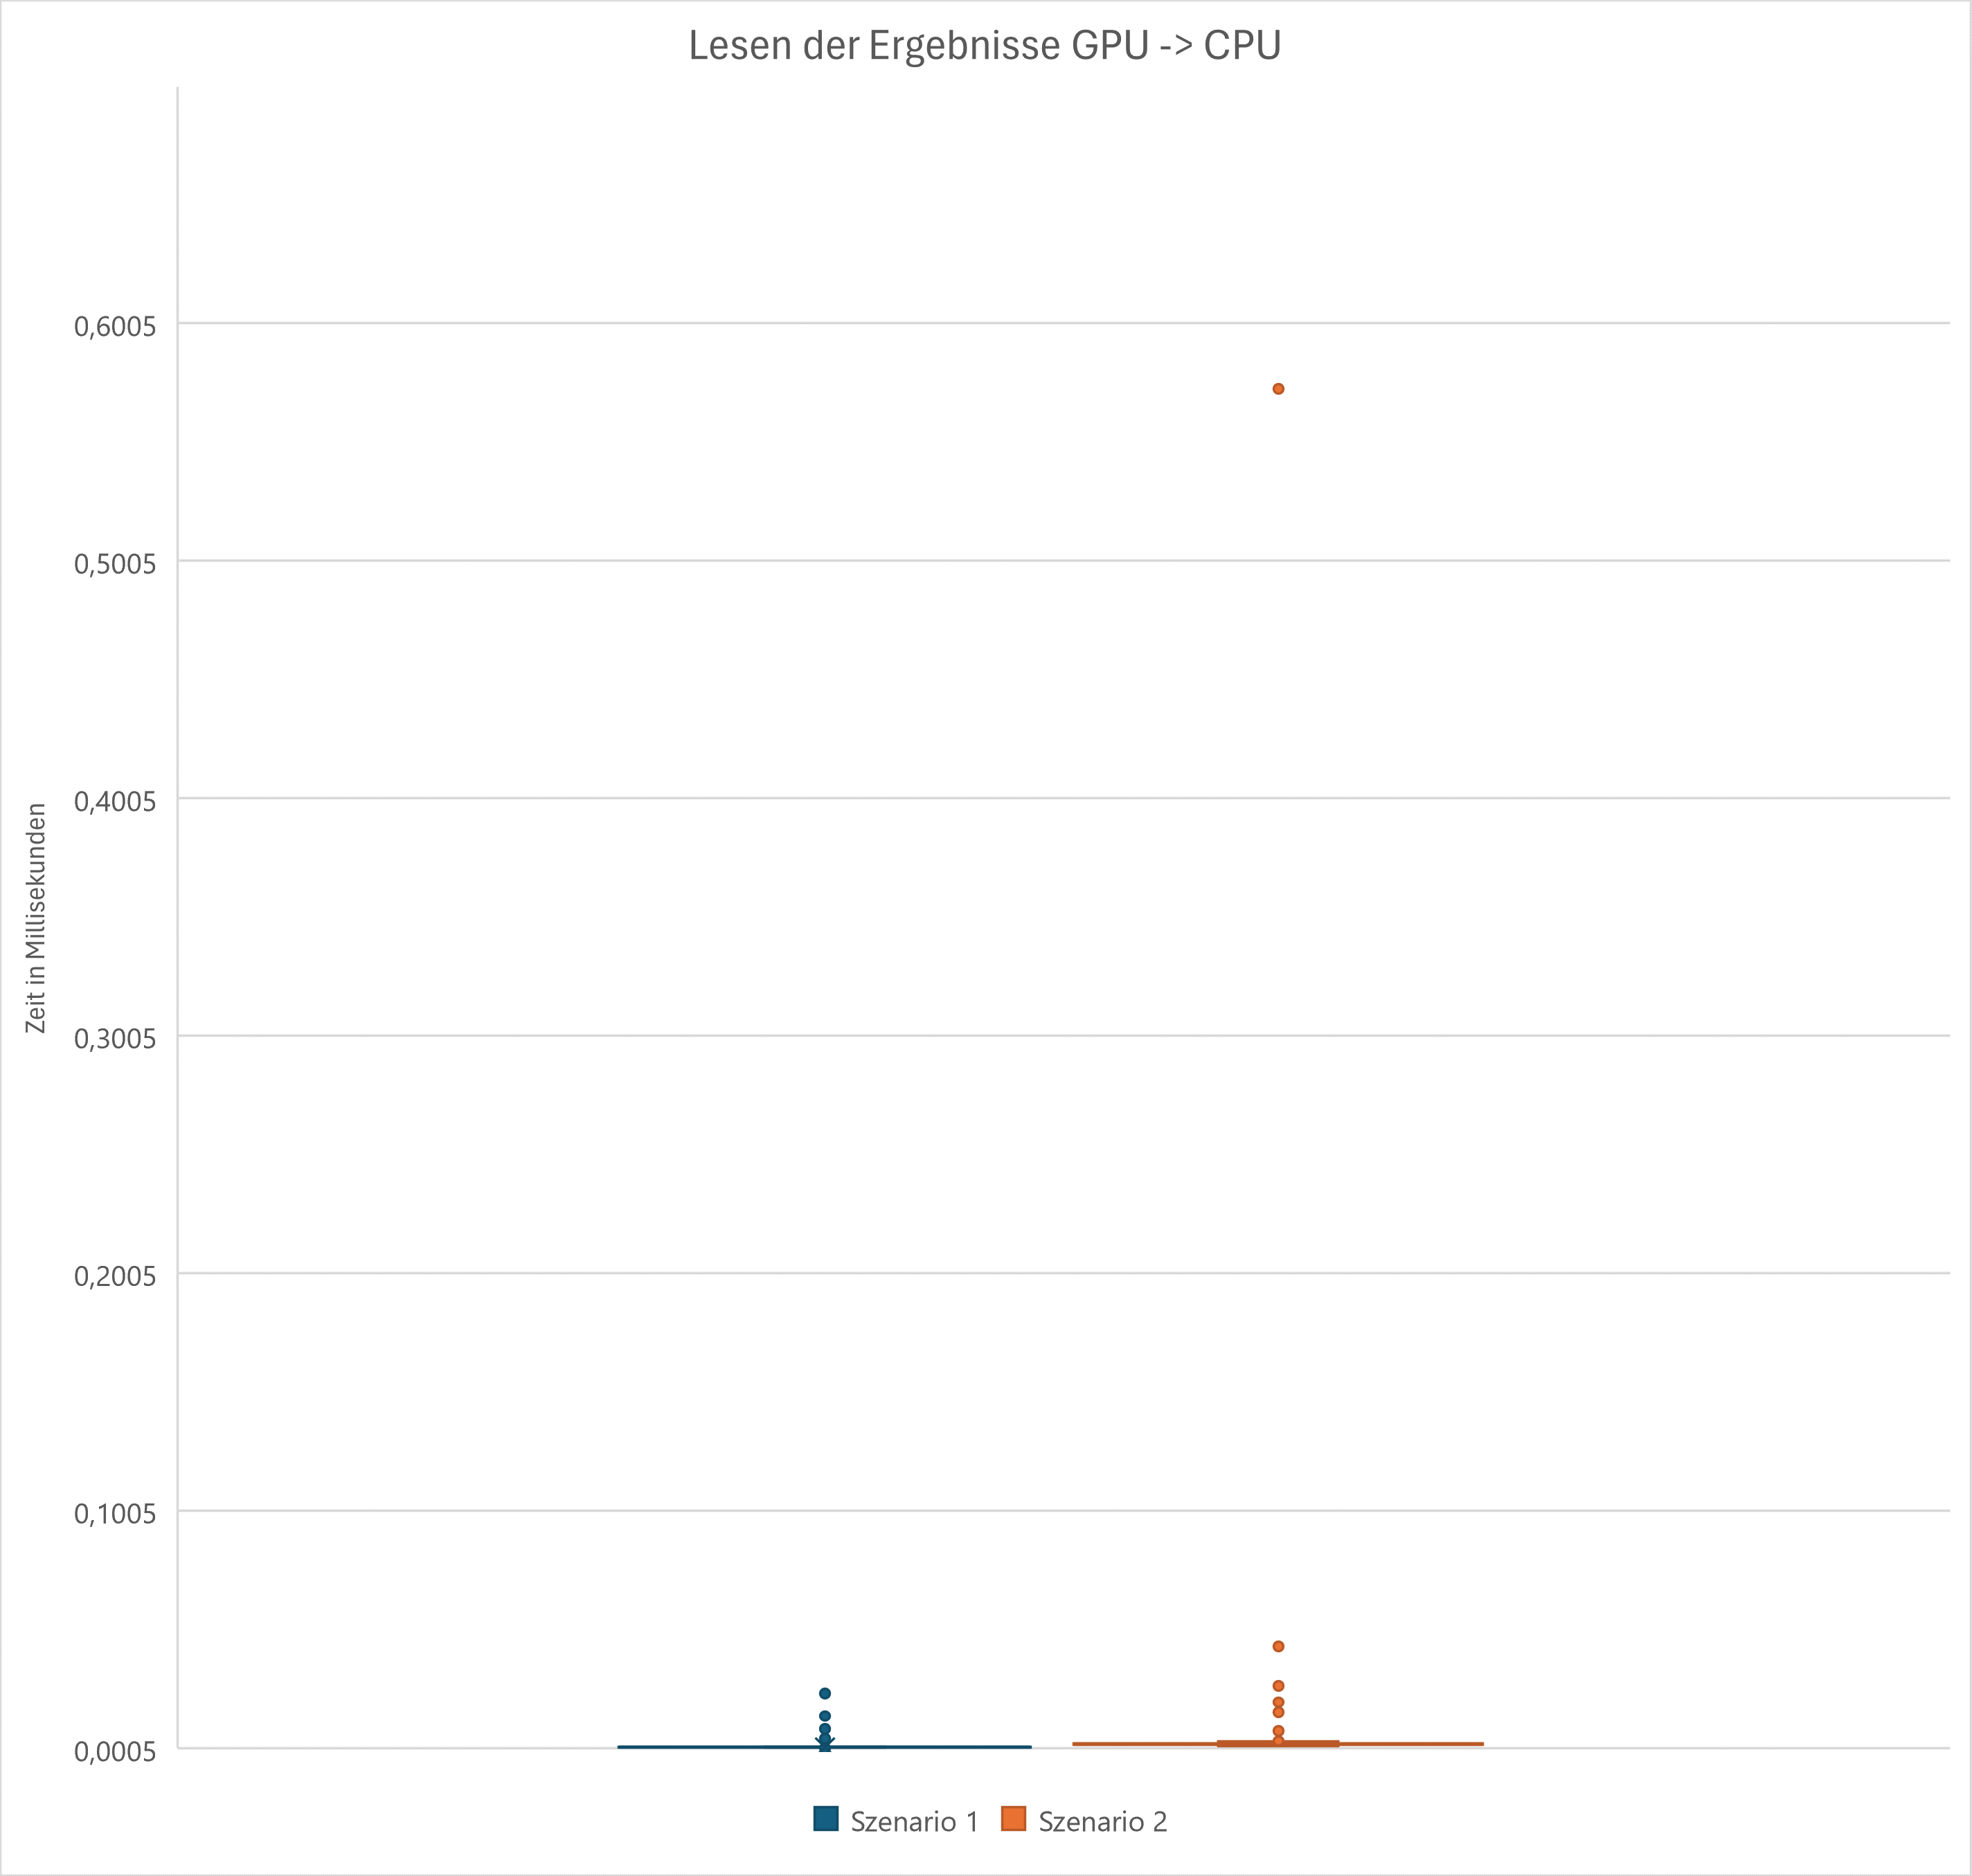
\includegraphics[width=0.7\linewidth]{Figures/rt_resultread_comp_outliers.png}
		\caption[Szenarienvergleich Transfer der Ergebnisse GPU->CPU mit Ausreißern]{Boxplots der benötigten Zeit zum Transfer der Ergebnisse von GPU->CPU beider Szenarien mit Ausreißern}
		\label{fig:resultscompoutliers}
	\end{figure}
	\pagebreak
	\appendixitem{Szenarienvergleich Bereinigung voriger BLAS \& TLAS mit Ausreißern}
	\begin{figure}[h!]
		\centering
		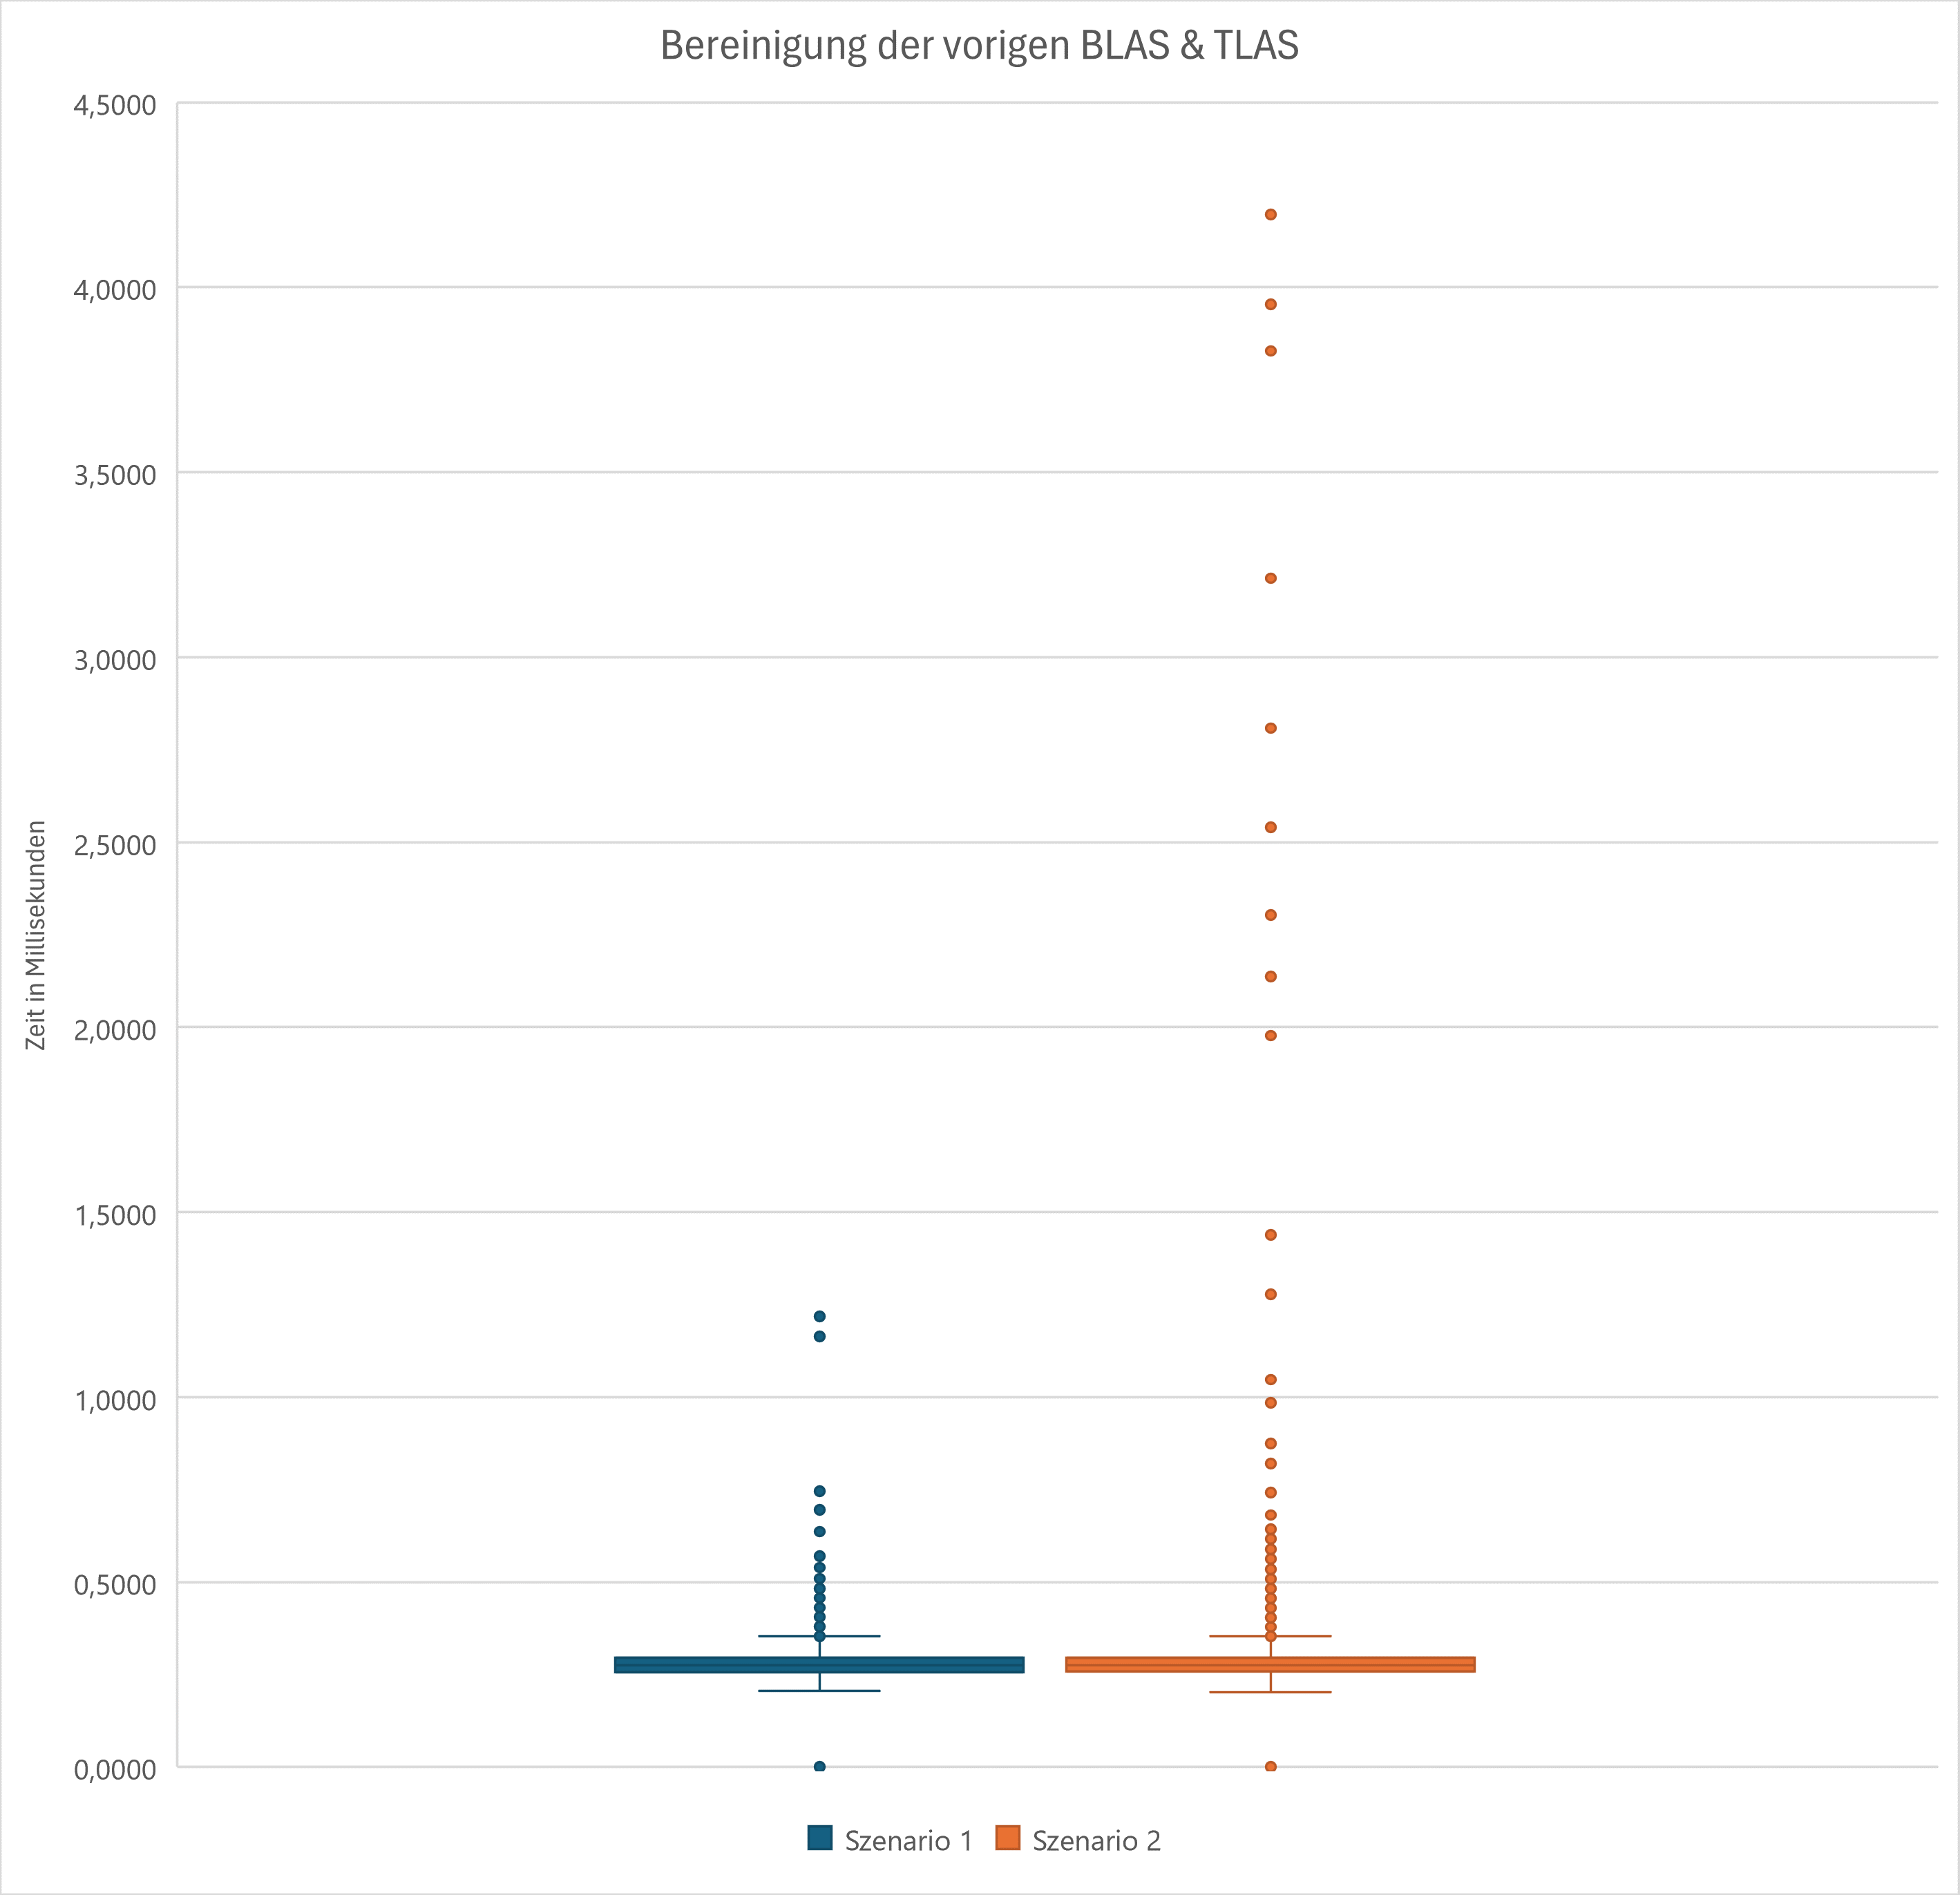
\includegraphics[width=0.7\linewidth]{Figures/rt_previous_cleanup_outliers.png}
		\caption[Szenarienvergleich Bereinigung voriger BLAS \& TLAS mit Ausreißern]{Boxplots der benötigten Zeit zum bereinigen der BLAS \& TLAS des vorigen Durchlaufs mit Ausreißern}
		\label{fig:cleanupcompoutliers}
	\end{figure}
	\pagebreak
	\appendixitem{Detaillierter Szenarienvergleich in UE5 mit Ausreißern}
	\begin{figure}[h!]
		\centering
		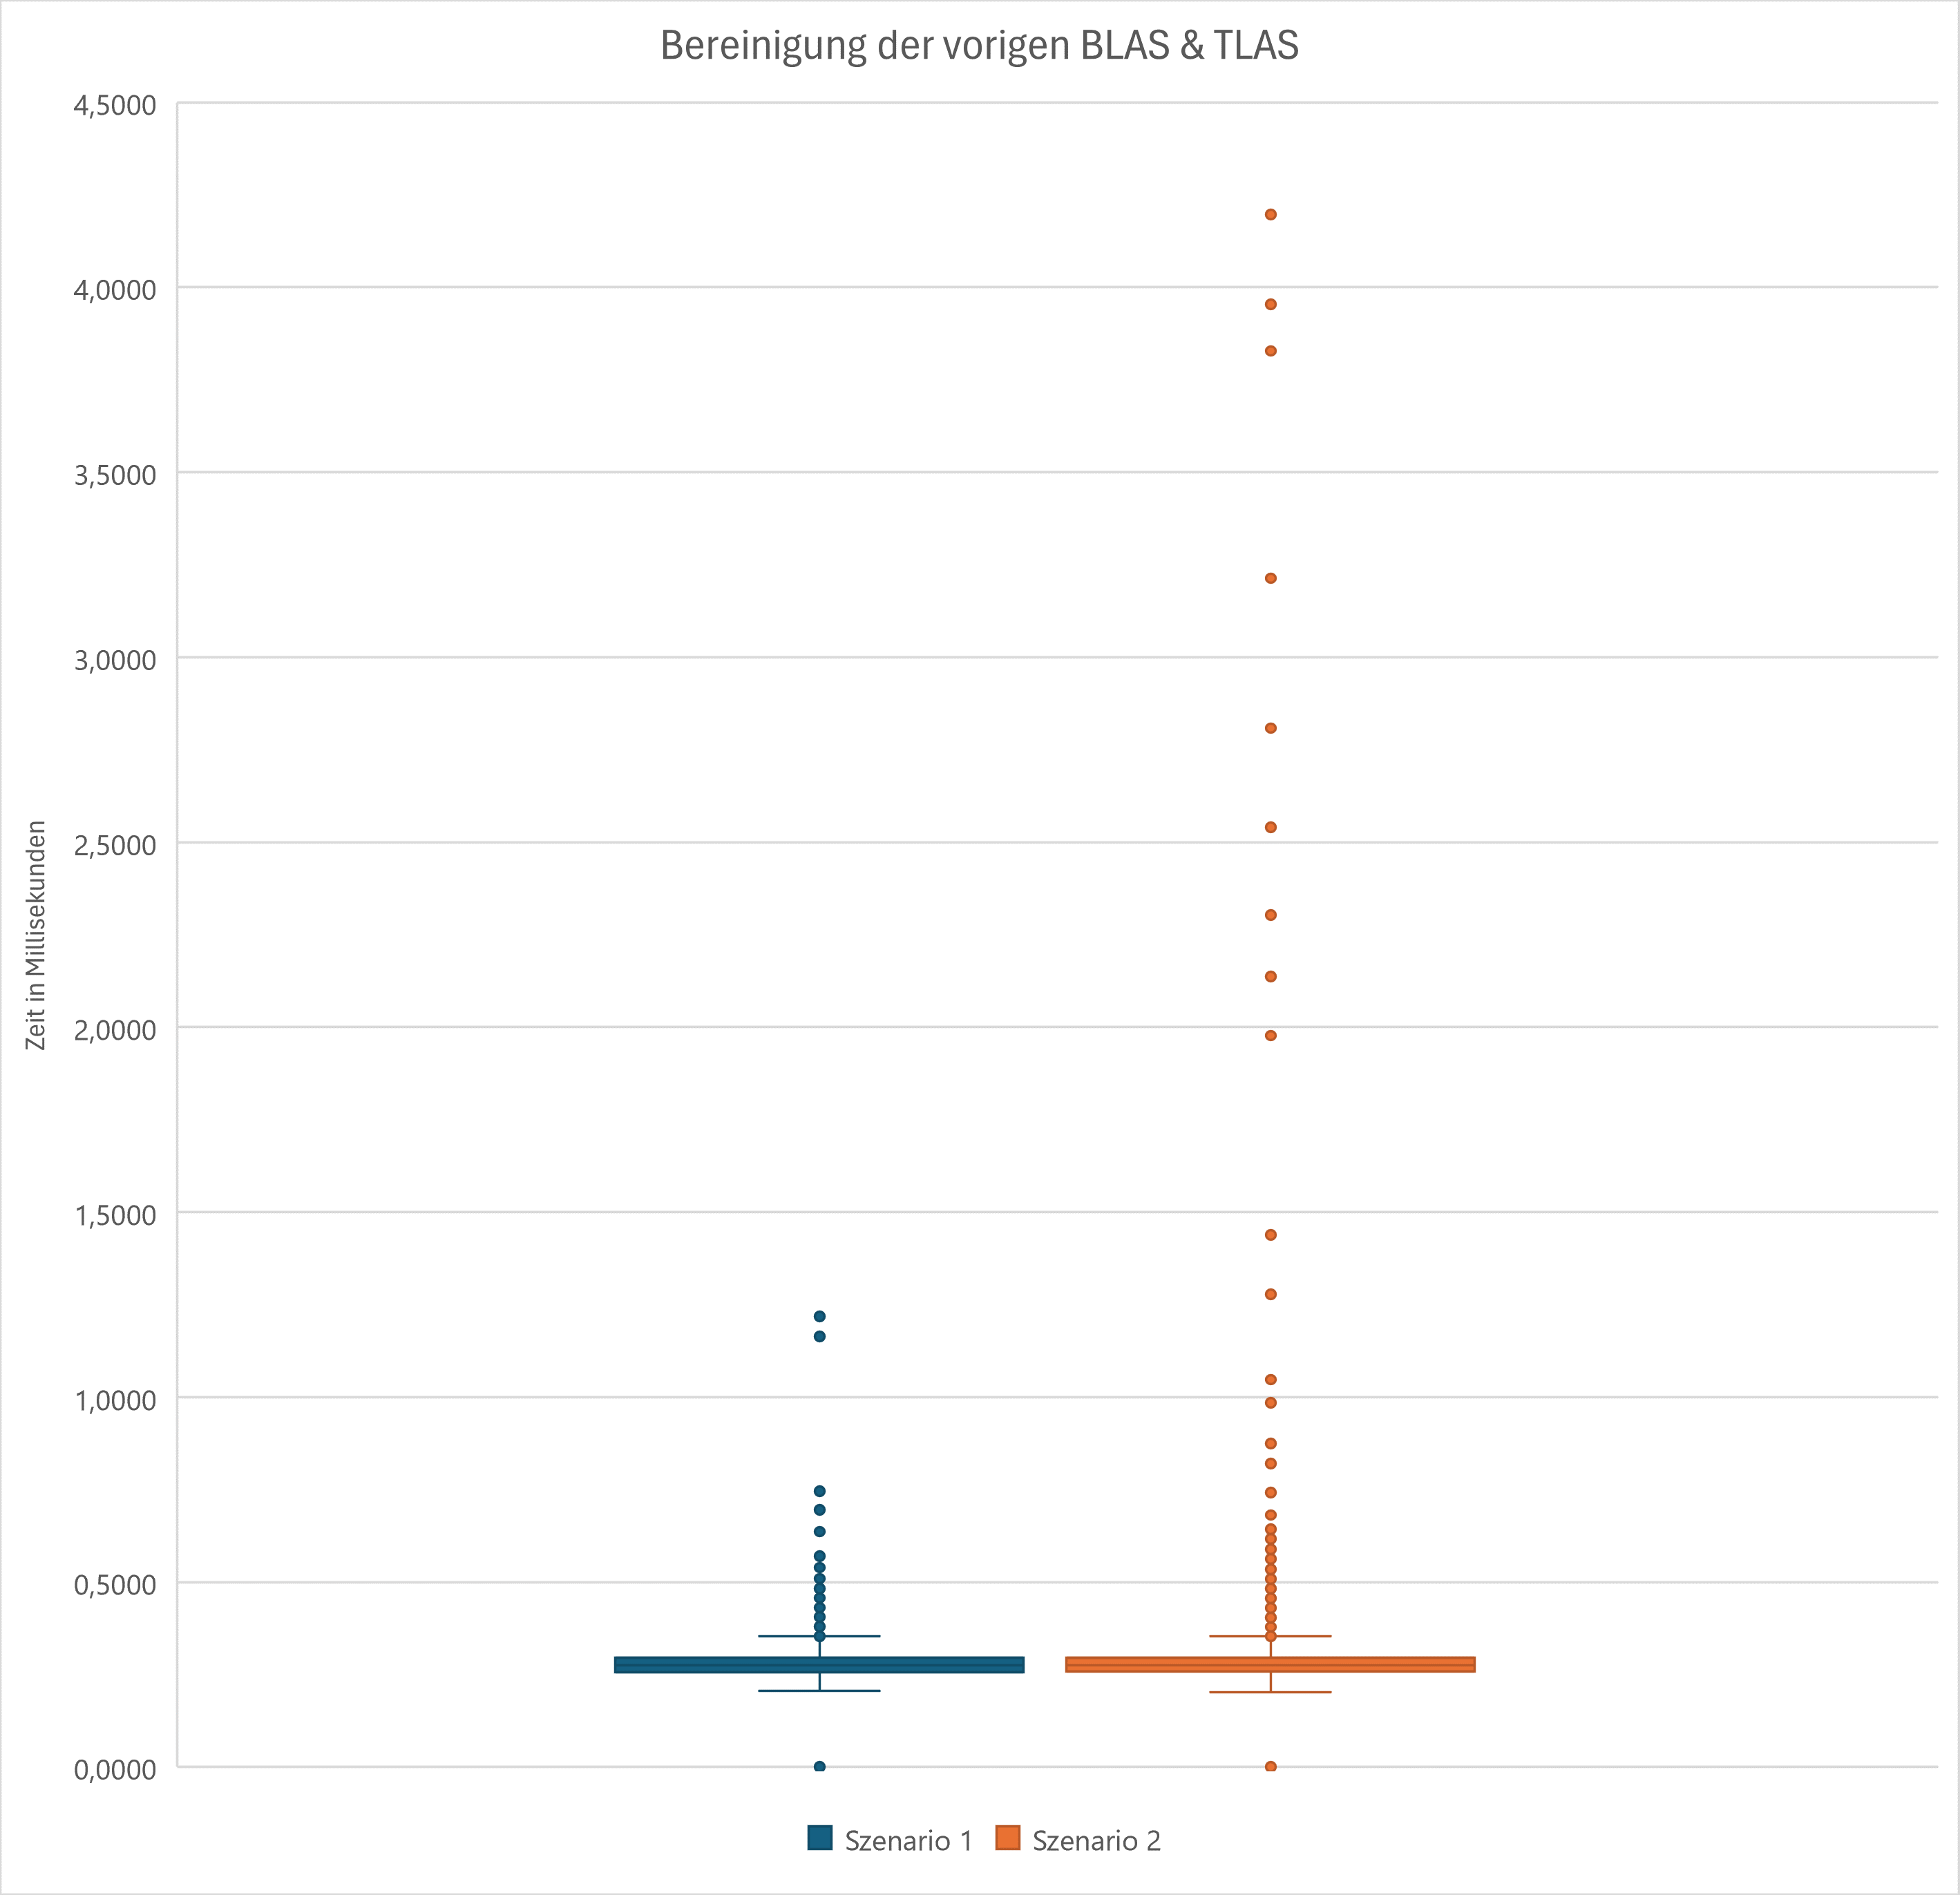
\includegraphics[width=0.7\linewidth]{Figures/rt_previous_cleanup_outliers.png}
		\caption[Detaillierter Szenarienvergleich in UE5 mit Ausreißern]{Boxplots der Szenarien und Varianten in UE5 mit Ausreißern}
		\label{fig:ue5compoutliers}
	\end{figure}
	
	\pagebreak
	
	\appendixitem{Erklärung über das eigenständige Erstellen der Arbeit}
	\noindent
	Hiermit versichere ich, dass ich die vorliegende Arbeit selbstständig verfasst und keine anderen als die angegebenen Quellen und Hilfsmittel benutzt habe. Die Stellen der Arbeit, die anderen Werken dem Wortlaut oder dem Sinn nach entnommen wurden, sind durch Angaben der Herkunft kenntlich gemacht.
	
	\noindent
	Diese Erklärung erstreckt sich auch auf in der Arbeit enthaltene Grafiken, Skizzen, bildliche Darstellungen sowie auf Quellen aus dem Internet.
	Die Arbeit habe ich in gleicher oder ähnlicher Form auch auszugsweise noch nicht als Bestandteil einer Prüfungs- oder Studienleistung vorgelegt. 
	
	\noindent
	Ich versichere, dass die eingereichte elektronische Version der Arbeit vollständig mit der Druckversion übereinstimmt.
	
	\medspace
	
	\noindent
	Name: \MetaAuthor\\\noindent
	Matrikelnummer: \MetaStudentNumber
	
	\thinspace
	
	\noindent
	Bremen, den \makebox[40mm]{\dotfill}
	
	\medspace
	
	\medspace
	
	\noindent
	\makebox[80mm]{\dotfill}\\
	(Unterschrift)

	
	
\end{document}
